%%%%%%%%%%%%%%%%%%%%%%%%%%%%%%%%%%%%%%%%%%%%%%%%%%%%%%%%%%%%%%%%%%%
%                                                                 %
%   HBOOK - Reference Manual -- LaTeX Source                      %
%                                                                 %
%   Main driver file. Includes other files of manual,             %
%                                                                 %
%   Files referenced: hbofront.tex   front material               %
%                     hbookch1.tex to hbooch10.tex                %
%                     hboomain.ind   index made with makeindex    %
%                     cnasbibl.bib   bibliography files (BibTeX)  %
%                                                                 %
%   To run, you need the CERN styles cernman.sty and crnman11.sty %
%                                                                 %
%   Editor: Michel Goossens / CN-AS                               %
%   Last Mod.: 13 June 1993 19:50  mg                             %
%                                                                 %
%%%%%%%%%%%%%%%%%%%%%%%%%%%%%%%%%%%%%%%%%%%%%%%%%%%%%%%%%%%%%%%%%%%

\documentstyle[longtable,epsfig,makeidx,cernhtml]{cernman}
\psfigdriver{HTML}
\makeindex
%\psdraft
\setlongtables
\PScommands% Initialize PS boxes
\let\Iind\Ropt
\newenvironment{Listing}%
{\begin{XMPt}{Output Generated}
\tiny}{\end{XMPt}}
\let\Listingp\Listing
\newmathalphabet*{\mathtt}{cmtt}{m}{n}
\newmathalphabet*{\mathbf}{cmr}{b}{n}
\pagestyle{empty}
\begin{document}
%  ==================== Front material ============================
\def\BIBFILE{H1Bibliography}
\Filename{HBOOKMAIN}
%%%%%%%%%%%%%%%%%%%%%%%%%%%%%%%%%%%%%%%%%%%%%%%%%%%%%%%%%%%%%%%%%%%
%                                                                 %
%   HBOOK - Reference Manual -- LaTeX Source                      %
%                                                                 %
%   Front Material: Title page,                                   %
%                   Copyright Notice                              %
%                   Preliminary Remarks                           %
%                   Table of Contents                             %
%   EPS file      : cern15.eps, cnastit.eps                       %
%                                                                 %
%   Editor: Michel Goossens / CN-AS                               %
%   Last Mod.:  9 December 1993 11:40 mg                          %
%                                                                 %
%%%%%%%%%%%%%%%%%%%%%%%%%%%%%%%%%%%%%%%%%%%%%%%%%%%%%%%%%%%%%%%%%%%

%%%%%%%%%%%%%%%%%%%%%%%%%%%%%%%%%%%%%%%%%%%%%%%%%%%%%%%%%%%%%%%%%%%%
%    Tile page                                                     %
%%%%%%%%%%%%%%%%%%%%%%%%%%%%%%%%%%%%%%%%%%%%%%%%%%%%%%%%%%%%%%%%%%%%
\notHTML{\def\Ptitle#1{\special{ps: /Printstring (#1) def}
                       \epsfbox{/usr/local/lib/tex/ps/cnastit.eps}}}
\HTML{\def\Ptitle#1{<B>#1</B>}}
 
\begin{titlepage}
\notHTML{\vspace*{-23mm}}%
\notHTML{\mbox{\epsfig{file=/usr/local/lib/tex/ps/cern15.eps,height=30mm}}}%
\HTML{<IMG SRC="../cernlogo.gif">}%
\hfill
\raise8mm\hbox{\Large\bf CERN Program Library Long Writeup Y250}
\hfill\mbox{}
\HTML{<P>}
\begin{center}
\mbox{}\\[10mm]
\mbox{\Ptitle{HBOOK}}\\[2cm]
\HTML{<P>\\}
{\LARGE Reference Manual}\\[2cm]
\HTML{<P>\\}
{\LARGE Version 4.22}\\[3cm]
\HTML{<P>\\}
{\Large Application Software Group}\\[1cm]
{\Large Computing and Networks Division}\\[2cm]
\end{center}
\HTML{<P>}
\notHTML{\vfill}%
\begin{center}\Large CERN Geneva, Switzerland\end{center}
\end{titlepage}

\Filename{H1Preface}
\HTML{<H1>Preface</H1>}

%%%%%%%%%%%%%%%%%%%%%%%%%%%%%%%%%%%%%%%%%%%%%%%%%%%%%%%%%%%%%%%%%%%%
%    Copyright  page                                               %
%%%%%%%%%%%%%%%%%%%%%%%%%%%%%%%%%%%%%%%%%%%%%%%%%%%%%%%%%%%%%%%%%%%%
\HTML{\PRE}
\thispagestyle{empty}
\framebox[\textwidth][t]{\hfill\begin{minipage}{0.96\textwidth}%
\vspace*{3mm}\begin{center}Copyright Notice\end{center}
\parskip\baselineskip
{\bf HBOOK -- Statistical Analysis and Histogramming}
 
CERN Program Library entry {\bf Y250}
 
\copyright{} Copyright CERN, Geneva 1993
 
Copyright and any other appropriate legal protection of these
computer programs and associated documentation reserved in all
countries of the world.
 
These programs or documentation may not be reproduced by any
method without prior written consent of the Director-General
of CERN or his delegate.
 
Permission for the usage of any programs described herein is
granted apriori to those scientific institutes associated with
the CERN experimental program or with whom CERN has concluded
a scientific collaboration agreement.
 
Requests for information should be addressed to:
\vspace*{-.5\baselineskip}
\begin{center}
\tt\begin{tabular}{l}
CERN Program Library Office              \\
CERN-CN Division                         \\
CH-1211 Geneva 23                        \\
Switzerland                              \\
Tel.      +41 22 767 4951                \\
Fax.      +41 22 767 7155                \\
Bitnet:   CERNLIB@CERNVM                 \\
DECnet:   VXCERN::CERNLIB (node 22.190)  \\
Internet: CERNLIB@CERNVM.CERN.CH
\end{tabular}
\end{center}
\vspace*{2mm}
\end{minipage}\hfill}%end of minipage in framebox
\vspace{6mm}
\HTML{<P>}
 
{\bf Trademark notice: All trademarks appearing in this guide are acknowledged as such.}
\vfill
\HTML{<P>}
\begin{tabular}{l@{\quad}l@{\quad}>{\tt}l}
{\em Contact Person\/}:        & Ren\'e Brun /CN     & (BRUN\atsign     CERNVM.CERN.CH)\\[1mm]
{\em Technical Realization\/}: & Michel Goossens /CN & (michel.goossens\atsign cern.ch)\\[1cm]
{\em Edition -- June 1994}
\end{tabular}
\HTML{\ePRE}%
\newpage
 
%%%%%%%%%%%%%%%%%%%%%%%%%%%%%%%%%%%%%%%%%%%%%%%%%%%%%%%%%%%%%%%%%%%%
%    Introductory material                                         %
%%%%%%%%%%%%%%%%%%%%%%%%%%%%%%%%%%%%%%%%%%%%%%%%%%%%%%%%%%%%%%%%%%%%
\pagenumbering{roman}
\setcounter{page}{1}

\Filename{H2History}
\section*{History}

HBOOK is a Fortran\footnote{A C interface is also distributed by
the CERN Program Library, created using the tool f2h} callable 
package for histogramming and fitting.
It was originally developed in the 1970s and has since
undergone continuous evolution culminating
in the current version, HBOOK~4.
 
Many people have contributed to the design and development of HBOOK,
through discussions, comments and suggestions.
 
% Since the very beginning the main author and coordinator of the
% HBOOK program has been Ren\'e Brun. He still keeps a detailed interest in
% future developments, but the formal responsability for 
% the package now lies with Jamie Shiers.
Paolo Palazzi was involved in the original design.
D.~Lienart has been in charge of the parametrization part. 
Fred~James is the author of routine \Rind{HDIFF} and of the minimization
package Minuit, which forms the basis of the fitting routines.
The idea of Profile histograms has been taken from the HYDRA system.
The Column-wise-Ntuple routines were implemented by Fons Rademakers.
The multi-dimensional quadratic fit package \Rind{HQUAD} is the work of
John Allison.
J.~Linnemann and his colleagues of the D0 experiment contributed
the routine \Rind{HDIFFB}.
Pierre Aubert is the author of the routines to associate labels
with histograms.
Roger Barlow and Christine Beeston (OPAL) have developed the 
\Rind{HMCMLL} package.

\Filename{H2Preliminary-remarks}
\section*{Preliminary remarks}
 
This manual serves at the same time as a {\bf Reference manual}
and as a {\bf User Guide} for the HBOOK system.
After a short introductory chapter, where the basic ideas
are explained, the following chapters describe in detail
the calling sequences for the different user routines.
 
In this manual
examples are in {\tt monotype face} and strings to be input by the user 
are {\tt\underline{underlined}}.
In the index the page where a routine is defined is in {\bf bold},
page numbers where a routine is referenced are in normal type.

In the description of the routines a \Lit{*} following
the name of a parameter indicates that this is an {\bf output} parameter.
If another \Lit{*} precedes a parameter in the calling sequence, the
parameter in question is both an {\bf input} and {\bf output} parameter.

This document has been produced using \LaTeX~\cite{bib-LATEX}
with the \Lit{cernman} style option, developed at CERN. 
A gzip compressed PostScript file \Lit{hbook.ps.gz},
containing a complete printable version
of this manual, can be obtained from any CERN machine
by anonymous ftp as follows
(commands to be typed by the user are underlined):

\vspace*{3mm} 
\begin{XMP}
    \underline{ftp asis01.cern.ch}
    Trying 128.141.201.136...
    Connected to asis01.cern.ch.
    220 asis01 FTP server (Version 6.10 ...) ready.
    Name (asis01:username): \underline{anonymous}
    Password: \underline{your\_{}mailaddress}
    230 Guest login ok, access restrictions apply.
    ftp> \underline{cd cernlib/doc/ps.dir}
    ftp> \underline{get hbook.ps.gz}    (type \Ucom{get hbook.ps} for the uncompressed version)
    ftp> \underline{quit}
\end{XMP}

%%%%%%%%%%%%%%%%%%%%%%%%%%%%%%%%%%%%%%%%%%%%%%%%%%%%%%%%%%%%%%%%%%%%
%    Tables of contents ...                                        %
%%%%%%%%%%%%%%%%%%%%%%%%%%%%%%%%%%%%%%%%%%%%%%%%%%%%%%%%%%%%%%%%%%%%
\newpage
\tableofcontents
%\newpage
\listoffigures
\listoftables


%  ==================== Body of text ==============================
%	$Id$	
%%%%%%%%%%%%%%%%%%%%%%%%%%%%%%%%%%%%%%%%%%%%%%%%%%%%%%%%%%%%%%%%%%%
%                                                                 %
%   HBOOK User Guide -- LaTeX Source                              %
%                                                                 %
%   Chapter 1                                                     %
%                                                                 %
%   The following external EPS files are referenced:              %
%         hbbatch.eps, hbookc11.eps                               %
%                                                                 %
%   Editor: Michel Goossens / CN-AS                               %
%   Last Mod.: 20 October 1993  9:00 mg                           %
%                                                                 %
%%%%%%%%%%%%%%%%%%%%%%%%%%%%%%%%%%%%%%%%%%%%%%%%%%%%%%%%%%%%%%%%%%%

\chapter{Introduction}       
\label{HINTRO}
 
Data processing is an important aspect of particle physics experiments
since the volume of data to be handled is quite large, a single LEP 
experiment producing of the order of a terabyte of data per year.
As a result, every particle physics laboratory has a large data 
processing centre even though more than 50\% of the computation is
actually carried on in universities or other research establishments.  
Particle physicists from various countries are in close contact on 
a continental and world wide basis,
the information exchanged being mainly via preprints and conferences.
The similarities in experimental devices and problems, and the close
collaboration, favour the adoption of common software methodologies that
sometimes develop into widely used standard packages. 
Examples are the histograming, fitting and data presentation package HBOOK, its
graphic interface \HPLOT~\cite{bib-HIGZHPLOT} and the
Physics Analysis Workstation (\PAW) system~\cite{bib-PAW}, 
which have been developed at CERN.

HBOOK is a subroutine package to handle statistical distributions
(histograms and Ntuples) in a Fortran scientific computation environment. 
It presents results graphically on the line printer, and can
optionally draw them on graphic output devices via the \HPLOT{}
package.
\PAW{} integrates the functionalities of the \HBOOK{} 
and \HPLOT{} (and other) packages
into an interactive workstation environment and provides the 
user with a coherent and complete working environment, 
from reading a (mini)DST,
via data analysis to preparing the final data presentation.

These packages are available from the CERN Program Library 
(see the copyright page for conditions).
They are presently being used on several hundred different computer
installations throughout the world.

\section{Data processing flow in particle experiments}
\label{HDATPROC}

In the late sixties and early seventies a large fraction of particle 
physicists were active in bubble chamber physics.
The number of events they treated varied between a few hundreds (neutrino) 
to several tens of thousands (e.g. strong interaction spectroscopy). 
Normally users would reduce there raw ``measurement'' tapes
\index{DST}
after event reconstruction onto Data Summary Tapes (DST) and extract from
there mini and micro DSTs, which would then be used for analysis.
In those days a statistical analysis program SUMX~\cite{bib-SUMX}
would read each event and compile information into histograms,
two-dimensional scatter diagrams and `ordered lists'. Facilities were
provided (via data cards) to select subset of events according
to criteria and the user could add routines for computing, event by
event, quantities not immediately available.

Although the idea and formalism of specifying cuts and
selection criteria in a formal way were a very nice idea,
the computer technology of those days only allowed the data to be analysed
in batch mode on the CDC or IBM mainframes.
Therefore it was not always very practical to run several times
through the data and a more lightweight system 
HBOOK~\cite{bib-HBOOK1,bib-HBOOK2},
easier to learn and use, was soon developed.

It was in the middle seventies, when larger proton and electron
accelerators became available, that counter experiments 
definitively superseded bubble chambers and with them the amount of data
to be treated was now in the multi megabyte range. Thousands of
raw data tapes would be written, huge reconstruction programs would
extract interesting data from those tapes and transfer them to 
DSTs. Then, to make the analysis more manageable, various physicists
would write their own mini-DST, with a reduced fraction of the
information from the DST. They would run these (m,$\mu$)DSTs through
HBOOK, whose functionality had increased substantially
in the meantime~\cite{bib-HBOOK3,bib-HBOOK3R}.
Hence various tens of one- or two-dimensional histograms
would be booked in the initialization phase and the interesting
parameters would be read sequentially from the DST and
be binned in the histograms or scatter plots. 
Doing this was very efficient memory wise (although 2-dim.
histograms could still be very costly), but of course all correlations,
not explicitly plotted, were lost.

HBOOK in those days still had its own memory management, but with 
version~4~\cite{bib-HBOOK4}, which became available in 1984, the
ZEBRA data memory manager was introduced.
This not only allowed the use of all memory managament facilities of ZEBRA,
but at the same time it became possible to use the sequential 
FZ and random access RZ~\cite{bib-ZEBRA} input-output
possiblities of that system.
This allows ``histograms'' to be saved and transferred to other systems
in an easy way.
At about the same time Ntuples, somewhat similar in functionality to 
``events'' as written on a miniDST were implemented.
This way the complete correlation matrix between the various
Ntuple elements can be reconstructed at will. 
The last few years multi Mflop machines have become available
on the desktop, and ``farms'' of analysis machines are being set up
to ``interactively'' reconstruct events directly from the
raw data as registered in the experimental setup, hence bypassing the
``batch'' reconstruction step.
The first Ntuple implementation can be thought of as a static large
two-dimensional array, one dimension representing the number of events
and the other a number of characteristics (floating point numbers)
stored for each event. 
With the present version of HBOOK Ntuples can contain complex
substructures of different data types, which allow a certain dynamicity.
Moreover tools have been developed to dynamically share
data between various processes (Unix) or global sections (VMS).
This makes it now possible to sample events as they are registered 
in the experimental setup or, when the computing power is
available, to reconstruct, vizualise and analize events in real time
as they are recorded in the experimental apparatus.
It is expected that this will progressively eliminate the intermediate
Batch/DST analysis step and allow, with the help of Monte Carlo events 
and calibration data, an (almost) immediate response to the
data taking needs of a large experiment.

\section{HBOOK and its output options}
\label{HOUTOPTS}

The HBOOK system consists of a few hundred Fortran
subroutines which enable the user to symbolically define, fill and output
one- and two-dimensional density estimators, under the form
of {\bf histograms}, {\bf scatter-plots} and {\bf tables} and
to handle Ntuples.

\index{histogram}
\index{scatter-plot}
\index{table}
\index{Ntuple}

Some interesting features of HBOOK are:
\begin{UL}
\item The basic operations require the knowledge of just a few
      subroutine calls that can be learned in half an hour, reading a few
      pages of documentation.  
      The internal structure of the
      package is also such that the options that are not directly
      called by the user program are not loaded in memory.
\item Histograms and plots are represented on the line printer in a
      standard format that contains the picture and some numerical 
      information. 
      Several options are available to modify the presentation, 
      mainly in the case of one dimensional histograms.  
      By default, one histogram per page is printed,
      writing a possible common title, date, individual title, drawing
      the countour of the histogram between the minimum and maximum
      channel content, with the contents scale adjusted to fit in one
      page, followed by channel number, contents and scale, and some
      statistical information (entries, mean value, standard deviation
      and so on).  
      If the number of channels is greater than 100, the
      histogram is printed on several pages.
\item Printing options permit to add or suppress some information,
      choose a different graphic presentation and modify the mapping of
      histograms on output pages.  
      Histograms can also be printed with channels
      oriented along rows instead of columns, to avoid splitting the
      ones with many channels. 
      Logarithmic contents scale can be selected.
      Various alternative output choices are illustrated in the examples.
\end{UL}

About 120 subroutines are directly accessible to the user program, via
Fortran calls of the type

\begin{center}
\fbox{\Lit{CALL H.....(P1,P2,..)}}
\end{center}

This is the only interface between a Fortran program and the dynamic
data structure managed by HBOOK, which thus
remains hidden from the average user.

\subsection*{The functionality of HBOOK}
      
The various user routines of HBOOK can be subdivided by functionality
as follows:
\begin{DL}{Random number generation}
\item[Booking]
      Declare a one- or two-dimensional histogram or a Ntuple.
\item[Projections]
      Project two-dimensional distributions onto both axes.
\item[Ntuples]
      Way of writing micro data-summary-files for further
      processing. This allows projections of
      individual variables or correlation plots. Selection mechanisms
      may be defined.
\item[Function representation]
      Associates a real function of 1 or 2 variables to a histogram.
\item[Filling]
      Enter a data value into a given histogram, table or Ntuple.
\item[Access to information]
      Transfer of numerical values from HBOOK-managed memory to Fortran
      variables and back.
\item[Arithmetic operations]
      On histograms and Ntuples.
\item[Fitting]
      Least squares and maximum likelihood fits of
      parametric functions to histogramed data.
\item[Monte Carlo testing]
      Fitting with finite Monte Carlo statistics.
\item[Differences between histograms\quad]
      Statistical tests on the compatibility in shape between histograms
      using the Kolmogorov test.
\item[Parameterization]
      Expresses relationships between as linear combinations of elementary
      functions. 
\item[Smoothing]
      Splines or other algorithms.
\item[Random number generation]
      Based on experimental distributions.
\item[Archiving]
      Information is stored
      on mass storage for further reference in subsequent programs.
\item[Editing]
      Choice of the form of presentation of the histogramed data.
\end{DL}

\section{What you should know before you start}

The basic data elements of HBOOK are the {\bf histogram} (one-
and two-dimensional) and the {\bf Ntuple}. The user identifies
his data elements using a {\bf single integer}. Each of the
elements has a number of {\bf attributes} associated with it.
\index{histogram}
\index{Ntuple}

The package is organised as part of a {\bf library}, from which
at load time unsatisfied externals are searched and loaded.
In this way only those subroutines actually used will be
loaded, therefore minimising the space occupied in memory by the code.
Unfortunately, given the way Fortran
works and although the package is structured as much as possible in the
sense of selective loading, some unused subroutines will usually be
present.

\finalnewpage

HBOOK uses the ZEBRA \cite{bib-ZEBRA} data structure
management package to manage its memory (see chapter \ref{HMEMORYM}).
The working space of HBOOK is an array, allocated to the labelled
common \Lit{/PAWC/}.
\index{common {\tt/PAWC/}}\index{PAWC@{\tt/PAWC/} common}
In ZEBRA terms this is a ZEBRA store.
It is thus necessary to reserve as many locations as required with a
declarative statement in the main program.
The actual length of the common is defined most safely via 
a \Lit{PARAMETER} statement, as shown below:

\begin{center}
\begin{tabular}{|>{\tt}l|}
\hline
PARAMETER (NWPAWC = 50000)\\
COMMON /PAWC/ HMEMOR(NWPAWC)\\
\hline
\end{tabular}
\end{center}
\index{common {\tt/PAWC/}}\index{PAWC@{\tt/PAWC/} common}

Furthermore HBOOK must be informed of the storage 
limit via a call to \Rind{HLIMIT}.
This is discussed in detail in section \vref{HMEMORYS}.
In the case above this would correspond to

\begin{center}
\fbox{CALL HLIMIT(NWPAWC)}
\end{center}
\Rind[HLIMIT]{}
 
At execution time, when histograms are booked, they are accomodated
in common \Lit{/PAWC/} in booking order, up to the maximum size available.
\index{common {\tt/PAWC/}}\index{PAWC@{\tt/PAWC/} common}

Note that a call to \Rind{HLIMIT} will automatically initialise the ZEBRA system
via a call to the routine \Rind{MZEBRA}.
If ZEBRA has already been initialised, (\Rind{MZEBRA} has already been called),
then \Rind{HLIMIT} should be called with a
{\bf negative} number indicating the number of words required, e.g.

\begin{center}
\fbox{CALL HLIMIT(-NWPAWC)}
\end{center}
\Rind[HLIMIT]{}

\subsection{HBOOK parameter conventions}

\subsubsection*{Histogram or Ntuple Identiers}
 
Histograms and Ntuples in HBOOK are identified by a positive 
or negative integer.
Thus the histogram identifier \Lit{ID = 0} is illegal at {\bf booking} time.
However it is a convenient way to specify that the option or operation
applies to {\bf all} known histograms in the current
working directory (e.g. output, input, printing).
All routines for which a zero identifier is meaningful
are mentioned explicitly.
\index{histogram!identifier}
\index{Ntuple!identifier}
\index{identifier}

\subsubsection*{Parameter types}

In agreement with the Fortran standard, when calling an
HBOOK routine the type of each parameter must correspond to
the one described in the routine's calling sequence in this manual.
Unless explicitly stated otherwise, parameters whose  names
start with \Lit{I, J, K, L, M} or \Lit{N} are {\bf integer}, 
the rest {\bf real}, with the exception of those beginning 
with the string \Lit{CH}, which correspond to character constants. 
\index{parameter type}
\index{Fortran convention}
\index{real type}
\index{character  type}
\index{integer type}
\index{type!parameter}
\index{type!real}
\index{type!character type}
\index{type!integer}

\subsubsection*{Data packing}
\index{packing}
\index{VMX@{\tt VMX}}

All booking commands that reserve space for histograms or plots
require the ``packing'' parameter \Lit{VMX}.
It corresponds to the 
estimated maximum population of a single bin,
on the basis of which a suitable number of bits per channel will be
allocated.
This allows several channels to be packed in one machine word,
and thus to require less storage space (at the expense of packing
and unpacking processing time).
A value \Lit{VMX=0.0} signals that no packing is to be performed
and that each histogram channel will occupy one machine word.

\finalnewpage

\section{A basic example}
\label{HSIMPLEXA}

Below a simple example is given describing 
how to use HBOOK for booking, filling and printing simple histograms.
After telling HBOOK the length of the \Lit{/PAWC/} common block
\index{common {\tt/PAWC/}}\index{PAWC@{\tt/PAWC/} common}
to be \Lit{10000} words with a call to \Rind{HLIMIT}, a 
global title to appear on all histograms is specified by calling
\Rind{HTITLE}. 
Next a 100 bin one-dimensional histogram with identifier 10 is booked 
with a call to \Rind{HBOOK1}, followed by the booking 
using a call to \Rind{HBOOK2} of a two-dimensional histogram with identifier 20 
and consisting of 100 times 40 cells.
The \Lit{DO}-loop labelled 10 fills the one-dimensional histogram 10,
while the nested \Lit{DO} loops labelled 20 and 30 look after filling
the two-dimensional histogram 20. 
In both cases a call is made to routine \Rind{HFILL}.
Finally a call to \Rind{HISTDO} writes an index with information 
about all histograms as well as a lineprinter representation of
the histograms on standard output.

\begin{XMPt}{Example of how to produce simple histograms}
      PROGRAM HSIMPLE
*
      PARAMETER (NWPAWC = 10000)
      COMMON/PAWC/H(NWPAWC)
*.___________________________________________
      CALL HLIMIT(NWPAWC)
*                       Set global title
*
      CALL HTITLE('EXAMPLE NO = 1')
*                       Book 1-dim histogram and scatter-plot
*
      CALL HBOOK1(10,'EXAMPLE OF 1-DIM HISTOGRAM',100,1.,101.,0.)
      CALL HBOOK2(20,'EXAMPLE OF SCATTER-PLOT',100,0.,1.,40,1.,41.,30.)
*                       Fill 1-dim histogram
*
      DO 10 I=1,100
         W=10*MOD(I,25)
         CALL HFILL(10,FLOAT(I)+0.5,0.,W)
  10  CONTINUE
*                       Fill scatter-plot
*
      X=-0.005
      DO 30 I=1,100
         X=X+0.01
         DO 20 J=1,40
            Y=J
            IW=MOD(I,25)*MOD(J,10)
            IWMAX=J-MOD(I,25)+10
            IF(IW.GT.IWMAX)IW=0
            CALL HFILL(20,X,Y,FLOAT(IW))
  20     CONTINUE
  30  CONTINUE
*                       Print all histograms with an index
*
      CALL HISTDO
      END
\end{XMPt}
\finalnewpage%%%%%%%%%%%%%%%%%%%%%%%%%%%%%%%%%%%%%%%%%%%%%%%%%%%%%%%%%%%%%%%%%%%%%%%%%%%%%%%%%%%%%%
\begin{Listing}
 EXAMPLE NO = 1
 
 .............................................................................................................................
 .                                                                                                                           .
 .   HBOOK   HBOOK  CERN            VERSION   4.13       HISTOGRAM AND PLOT INDEX                             17/12/91       .
 .                                                                                                                           .
 .............................................................................................................................
 .                                                                                                                           .
 .  NO                     TITLE                      ID  B/C  ENTRIES DIM   NCHA     LOWER       UPPER       ADDRESS LENGTH .
 .                                                                                                                           .
 .............................................................................................................................
 .                                                                                                                           .
 .                                                                                                                           .
 .   1  EXAMPLE OF 1-DIM HISTOGRAM                    10  32      100  1  X   100   0.100E+01   0.101E+03       79369    149 .
 .                                                                                                                           .
 .                                                                                                                           .
 .   2  EXAMPLE OF SCATTER-PLOT                       20   5     4000  2  X   100   0.000E+00   0.100E+01       79217    760 .
 .                                                                        Y    40   0.100E+01   0.410E+02       78482    726 .
 .                                                                                                                           .
 .............................................................................................................................

 MEMORY UTILISATION

      MAXIMUM TOTAL SIZE OF COMMON /PAWC/            80000
\newpage\setlength{\baselineskip}{5.7pt}\relax
 EXAMPLE NO = 1                                                                  
 --------------                                                                  
 EXAMPLE OF 1-DIM HISTOGRAM                                                      
 
 HBOOK     ID =        10                                        DATE  17/12/91              NO =   1
 
      250
      240                              -                        -                        -                        -
      230                             -I                       -I                       -I                       -I
      220                            -II                      -II                      -II                      -II
      210                           -I I                     -I I                     -I I                     -I I
      200                          -I  I                    -I  I                    -I  I                    -I  I
      190                         -I   I                   -I   I                   -I   I                   -I   I
      180                        -I    I                  -I    I                  -I    I                  -I    I
      170                       -I     I                 -I     I                 -I     I                 -I     I
      160                      -I      I                -I      I                -I      I                -I      I
      150                     -I       I               -I       I               -I       I               -I       I
      140                    -I        I              -I        I              -I        I              -I        I
      130                   -I         I             -I         I             -I         I             -I         I
      120                  -I          I            -I          I            -I          I            -I          I
      110                 -I           I           -I           I           -I           I           -I           I
      100                -I            I          -I            I          -I            I          -I            I
       90               -I             I         -I             I         -I             I         -I             I
       80              -I              I        -I              I        -I              I        -I              I
       70             -I               I       -I               I       -I               I       -I               I
       60            -I                I      -I                I      -I                I      -I                I
       50           -I                 I     -I                 I     -I                 I     -I                 I
       40          -I                  I    -I                  I    -I                  I    -I                  I
       30         -I                   I   -I                   I   -I                   I   -I                   I
       20        -I                    I  -I                    I  -I                    I  -I                    I
       10       -I                     I -I                     I -I                     I -I                     I
 
 CHANNELS 100   0                                                                                                  1   
           10   0        1         2         3         4         5         6         7         8         9         0   
            1   1234567890123456789012345678901234567890123456789012345678901234567890123456789012345678901234567890   
 
 CONTENTS 100            111111111122222          111111111122222          111111111122222          111111111122222 
           10   123456789012345678901234 123456789012345678901234 123456789012345678901234 123456789012345678901234 
            1.  000000000000000000000000 000000000000000000000000 000000000000000000000000 000000000000000000000000 
 
 LOW-EDGE 100                                                                                                      1
           10            1111111111222222222233333333334444444444555555555566666666667777777777888888888899999999990
            1.  1234567890123456789012345678901234567890123456789012345678901234567890123456789012345678901234567890
 
 * ENTRIES =        100      * ALL CHANNELS = 0.1200E+05      * UNDERFLOW = 0.0000E+00      * OVERFLOW = 0.0000E+00
 * BIN WID = 0.1000E+01      * MEAN VALUE   = 0.5433E+02      * R . M . S = 0.2854E+02

\finalnewpage

 EXAMPLE NO = 1                                                                  
 --------------                                                                  
 
 EXAMPLE OF SCATTER-PLOT                                                         
 
 HBOOK     ID =        20                                        DATE  17/12/91              NO =   2
 
 CHANNELS 100 U 0                                                                                                  1 O 
           10 N 0        1         2         3         4         5         6         7         8         9         0 V 
            1 D 1234567890123456789012345678901234567890123456789012345678901234567890123456789012345678901234567890 E 
            ************************************************************************************************************
   OVE      *                                                                                                          * OVE
    40      *                                                                                                          *  40
    39      *   9IR*                     9IR*                     9IR*                     9IR*                        *  39
    38      *   8GO**                    8GO**                    8GO**                    8GO**                       *  38
    37      *   7ELS*                    7ELS*                    7ELS*                    7ELS*                       *  37
    36      *   6CIOU*                   6CIOU*                   6CIOU*                   6CIOU*                      *  36
    35      *   5AFKPU*                  5AFKPU*                  5AFKPU*                  5AFKPU*                     *  35
    34      *   48CGKOS*                 48CGKOS*                 48CGKOS*                 48CGKOS*                    *  34
    33      *   369CFILORU               369CFILORU               369CFILORU               369CFILORU                  *  33
    32      *   2468ACEGIKMOQS           2468ACEGIKMOQS           2468ACEGIKMOQS           2468ACEGIKMOQS              *  32
    31      *   +23456789ABCDEFGHIJK     +23456789ABCDEFGHIJK     +23456789ABCDEFGHIJK     +23456789ABCDEFGHIJK        *  31
    30      *                                                                                                          *  30
    29      *   9IR                      9IR                      9IR                      9IR                         *  29
    28      *   8GO*                     8GO*                     8GO*                     8GO*                        *  28
    27      *   7ELS                     7ELS                     7ELS                     7ELS                        *  27
    26      *   6CIOU                    6CIOU                    6CIOU                    6CIOU                       *  26
    25      *   5AFKP                    5AFKP                    5AFKP                    5AFKP                       *  25
    24      *   48CGKO                   48CGKO                   48CGKO                   48CGKO                      *  24
    23      *   369CFILO                 369CFILO                 369CFILO                 369CFILO                    *  23
    22      *   2468ACEGIK               2468ACEGIK               2468ACEGIK               2468ACEGIK                  *  22
    21      *   +23456789ABCDEF          +23456789ABCDEF          +23456789ABCDEF          +23456789ABCDEF             *  21
    20      *                                                                                                          *  20
    19      *   9I                       9I                       9I                       9I                          *  19
    18      *   8GO                      8GO                      8GO                      8GO                         *  18
    17      *   7EL                      7EL                      7EL                      7EL                         *  17
    16      *   6CI                      6CI                      6CI                      6CI                         *  16
    15      *   5AFK                     5AFK                     5AFK                     5AFK                        *  15
    14      *   48CG                     48CG                     48CG                     48CG                        *  14
    13      *   369CF                    369CF                    369CF                    369CF                       *  13
    12      *   2468ACE                  2468ACE                  2468ACE                  2468ACE                     *  12
    11      *   +23456789A               +23456789A               +23456789A               +23456789A                  *  11
    10      *                                                                                                          *  10
     9      *   9                        9                        9                        9                           *   9
     8      *   8G                       8G                       8G                       8G                          *   8
     7      *   7E                       7E                       7E                       7E                          *   7
     6      *   6C                       6C                       6C                       6C                          *   6
     5      *   5A                       5A                       5A                       5A                          *   5
     4      *   48                       48                       48                       48                          *   4
     3      *   369                      369                      369                      369                         *   3
     2      *   2468                     2468                     2468                     2468                        *   2
     1      *   +2345                    +2345                    +2345                    +2345                       *   1
   UND      *                                                                                                          * UND
            ************************************************************************************************************
 LOW-EDGE   0   0000000000111111111122222222223333333333444444444455555555556666666666777777777788888888889999999999
            0   0123456789012345678901234567890123456789012345678901234567890123456789012345678901234567890123456789
 
  *                                                          I         I
  * ENTRIES =     4000                   PLOT       ---------I---------I---------
  * SATURATION  AT=           31                             I    10488I
  * SCALE  .,+,2,3,.,., A,B,           STATISTICS   ---------I---------I---------
  * STEP = 1.00     * MINIMUM=0.000                          I         I
\end{Listing}

\finalnewpage%%%%%%%%%%%%%%%%%%%%%%%%%%%%%%%%%%%%%%%%%%%%%%%%%%%%%%%%%%%%%%%%%%%%%%%%%%%%%%%%%%%

\section{HBOOK batch as the first step of the analysis}

%begin{latexonly}
\begin{Fighere}
\centering\includegraphics[width=125mm]{hbbatch.eps}
\caption{Schematic presentation of the various steps in the data analysis chain}
\label{FBATCH}
\end{Fighere}
%end{latexonly}
\begin{htmlonly}
\begin{figure}
\begin{makeimage}
\includegraphics[width=125mm]{hbbatch.eps}
\end{makeimage}
\caption{Schematic presentation of the various steps in the data analysis chain}
\label{FBATCH}
\end{figure}
\end{htmlonly}

Although it is possible to define histograms interactively in a PAW
session, and then read the (many thousands of) events, in general
for large data samples the relevant variables are extracted from
the {\bf Data Summary Files {\rm or} DST}s
and stored in {\bf histograms}
\index{DST}
or an {\bf Ntuple}.
Histograms require to make a certain choice 
as to the range of values for the plotted parameter, because the
{\bf binning}, or the coarseness, of the distribution has to
be specified when the histogram is defined ({\bf booked}).
Also only one- and two-dimensional histograms are possible, hence the
correlations between various parameters can be difficult to study.
Hence in many cases it is more appropriate to store the value of
the important parameters for each event in an {\bf Ntuple}.
This approach preserves the correlation between the parameters
and allows selection criteria to be applied on the (reduced)
data sample at a later stage.

In general, the time consuming job of
analysing all events available on tape is run on a mainframe or CPU 
server, and
the important event parameters are stored in a Ntuple
to allow further detailed study. For convenience the Ntuple
can be output to disk for each run, and then at a later stage the
Ntuples can be {\bf merged} in order to allow a global
interactive analysis of the complete data sample (see Figure \ref{FBATCH}).

%\vspace*{\baselineskip}

A typical batch job in which data are analysed offline and
some characteristics are stored in HBOOK is shown in Figure~\ref{FEX1IN}.
HBOOK is initialised by a call to~\Lit{HLIMIT}, 
which declares a length of 20000 words for the
length of the \Lit{/PAWC/} dynamic store. Then the one- and two-
dimensional histograms 110 and 210 are filled respectively
according to the functions \Lit{HTFUN1} and \Lit{HTFUN2}
and the histograms are output to a newly created file \Lit{HTEST.DAT}.
The output generated by the program is shown in Figure~\ref{FEX1OU}.

\begin{figure}[p]
\begin{XMPfont}{8}
      PROGRAM HTEST
      PARAMETER (NWPAWC=20000)
      COMMON/PAWC/H(NWPAWC)
      EXTERNAL HTFUN1,HTFUN2
*.------------------------------------------------------------
      CALL HLIMIT(NWPAWC)
*             Book histograms and declare functions
      CALL HBFUN1(100,'Test of HRNDM1',100,0.,1.,HTFUN1)
      CALL HBOOK1(110,'Filled according to HTFUN1',100,0.,1.,1000.)
      CALL HBFUN2(200,'Test of HRNDM2',100,0.,1.,40,0.,1.,HTFUN2)
      CALL HSCALE(200,0.)
      CALL HBOOK2(210,'Filled according to HTFUN2',100,0.,1.,40,0.,1.,30.)
*             Fill histograms
      DO 10 I=1,10000
         X=HRNDM1(100)
         CALL HFILL(110,X,0.,1.)
         CALL HRNDM2(200,X,Y)
         CALL HFILL(210,X,Y,1.)
  10  CONTINUE
*             Save all histograms on file HTEST.DAT
      CALL HRPUT(0,'HTEST.DAT','N')
      CALL HDELET(100)
      CALL HDELET(200)
      CALL HPRINT(0)
      END
      FUNCTION HTFUN2(X,Y)
*             Two-dimensional gaussian
      HTFUN2=HTFUN1(X)*HTFUN1(Y)
      RETURN
      END
 
      FUNCTION HTFUN1(X)
*             Constants for gaussians
      DATA C1,C2/1.,0.5/
      DATA XM1,XM2/0.3,0.7/
      DATA XS1,XS2/0.07,0.12/
*             Calculate the gaussians
      A1=-0.5*((X-XM1)/XS1)**2
      A2=-0.5*((X-XM2)/XS2)**2
      X1=C1
      X2=C2
      IF(ABS(A1).GT.0.0001)X1=C1*EXP(A1)
      IF(ABS(A2).GT.0.0001)X2=C2*EXP(A2)
*             Return function value
      HTFUN1=X1+X2
      RETURN
      END
\end{XMPfont}

\caption{Writing data to HBOOK with the creation of a HBOOK RZ file}
\label{FEX1IN}

\begin{minipage}[t]{.495\textwidth}
\begin{XMPfrac}{3.3}
Filled according to HTFUN1
 
HBOOK     ID =       110                                        DATE  02/09/89               NO =  2
 
     340                                    -
     330                                    I -
     320                                    I I
     310                                    I I
     300                                    I-I-
     290                                  --I  I
     280                                 -I    I-
     270                                 I      I
     260                                 I      I
     250                                -I      I-
     240                                I        I
     230                               -I        I
     220                               I         I-
     210                              -I          I
     200                              I           I -
     190                              I           I-I
     180                             -I             I
     170                             I              I                                -
     160                             I              I                          -    -I-   -
     150                             I              I-                         I  --I I- -I -
     140                             I               I-                       -I--I    I-II-I-
     130                           --I                I-                     -I              I
     120                           I                   I                  - -I               I
     110                           I                   I                  I-I                I--
     100                           I                   I-                -I                    I
      90                          -I                    I-              -I                     I----
      80                         -I                      I            --I                          I-
      70                         I                       I           -I                             I
      60                        -I                       I--       - I                              I- -
      50                       -I                          I-- ----I-I                               I-I-
      40                       I                             I-I                                        I---
      30                     --I                                                                           I--
      20                   --I                                                                               I --
      10            -------I                                                                                 I-II--
 
CHANNELS 100   0                                                                                                  1
          10   0        1         2         3         4         5         6         7         8         9         0
           1   1234567890123456789012345678901234567890123456789012345678901234567890123456789012345678901234567890
 
CONTENTS 100                       111222222323222211111                  1111111111111111111111
          10             1 12224578227034888392975189442985544344445467789101235335456543453430088887545443322111
           1.       22345055038484428230601947383077660674994445157562761227948358021717653142735611669210337304276
 
LOW-EDGE   1.            111111111122222222223333333333444444444455555555556666666666777777777788888888889999999999
*10**  1   0   0123456789012345678901234567890123456789012345678901234567890123456789012345678901234567890123456789
 
* ENTRIES =      10000      * ALL CHANNELS = 0.1000E+05      * UNDERFLOW = 0.0000E+00      * OVERFLOW = 0.0000E+00
* BIN WID = 0.1000E-01      * MEAN VALUE   = 0.4846E+00      * R . M . S = 0.2199E+00
\end{XMPfrac}   
\end{minipage}\hfill
\begin{minipage}[t]{.495\textwidth}
\begin{XMPfrac}{3.3}
Fill according to HTFUN2
 
HBOOK     ID =       210                                        DATE  02/09/89               NO =  4
 
CHANNELS 100 0                                                                                                  1
          10 0        1         2         3         4         5         6         7         8         9         0
           1 1234567890123456789012345678901234567890123456789012345678901234567890123456789012345678901234567890
           ********************************************************************************************************
  OVE      *                                                                                                      * OVE
     .975  *                                                                                                      *  40
     .95   *                  ++   2   2 2++  +3 +   ++     +  +     2+         3 2  + 2++++       + 2    +       *  39
     .925  *           +   +    2  ++ 32+++ +22  22+    +++    +       + +    +  22+2+++ +2++   + + +             *  38
     .9    *                   223 +3+ +3 3++333223  +2  2     +  +    ++2+ +    232+322 2+++  +24+      +        *  37
     .875  *           +   ++ +2++++ 342533 443224++2 2  +   +  ++23  +  +42+3222233+++3+++2 22+ ++   + + +       *  36
     .85   *               ++  + 5+35+3333483475 65+2+ + ++  +    +33+3 +2 +2335222+235 522 24+   ++    2         *  35
     .825  *                ++  2+2 558335876736583+ 2 +2+ + +   3   224+533623+35252+54 32+452++3 332 +++++      *  34
     .8    *            ++   + 532 656562546C8A88936324332+ +2+23 +332+2236433657234455556+4635+222 +23 +3  +     *  33
     .775  *               +2  33 375B7274C6A66A782+323++2+23  +5++3+5222256768365258276374+86334+ 32    +++ +    *  32
     .75   *            + 2+ 2 45523786A79FB98B6AD4855224+  + ++23323+5755552468283746644543 443324 5223++  2     *  31
     .725  *            + ++4+22+637A785B8BBBA6B4656922++ 2 23 24 2+5464+435552843286C6246623636+3+ 2 3 2  3+2    *  30
     .7    *       +      22 +2 735ABCA89G8C8A6DA5765+3+322  2+2++52234445475+355864768724+B74632+23 +3   3+   +  *  29
     .675  *              23 +4+3364HBBAFCFCBB98945C7933++ 2 5+3 +4225243752 75787896C367+475443+32242422 2 +     *  28
     .65   *           + + ++5+3795498GAC96CB9A79E6645 34 3+3  ++24537234424532777657445+4746235+2+3++  4+2 2     *  27
     .625  *           +     3 647774A9CE67G99BAB6B233233 4+ 2 322 42 44364+657735+735736733+4+23234 +++++2  +    *  26
     .6    *            + ++3+342233874B8C966896565+5242+5 +2+++++2+5225+42544535456A265357253+2222+ 2+2++ +  +2  *  25
     .575  *           ++  +  +5 74535525677984573453422 +2   ++ 2  +++4+2 3526525235+4243342+32+  23 2+          *  24
     .55   *               ++ +226+584568349865+433 +2222 +      ++ +4444352326542332823+444332 +2 2 + +          *  23
     .525  *                 ++++2+65436+3A753535+22+++2+++  ++ + ++2  +2 ++4++2+ 224224+32 2+ ++++ 2      +      *  22
     .5    *                 22  4+23+6425 84543+++42 +2     +++2  2 + 2+2+ 3+ 24++2334223+ 223  +2   +       +   *  21
     .475  *         +             +5334+7333+22  ++2+ +  3+      2 +4 +32  2 222+2 + 33++ 222 +  +3++     +      *  20
     .45   *                  +  433244397 2++23232+ 24 +2        ++  ++2+ 2+ +2+33  ++4 +3 ++2+3    +  +         *  19
     .425  *           +  ++ 2+ 22+24636432646+5+322 4 +++ + 2++  ++ +22+533+3++3+  +432 +322++2+     2+  ++ +    *  18
     .4    *                +++3237549588A9725H724545++33+33 + + 2 24  4 +A4633 39 25636343322+82++ ++ + +2+  +   *  17
     .375  *              +++3+374879CCCADLD48996CE54365232 +2+2342347+563264636547B47925542444434+2+322 2+  +2   *  16
     .35   *            +++ +4637549EC87D8IHDICI9B754655432++23233+2554368886H68B9667889677A635C+4+223333+22  +   *  15
     .325  *        +  ++++ 2445949CHHDFNHJRHIHKLDD5DC3545422233 24564875549A8E7899B4F4BC3CA7E597842+67242+++++   *  14
     .3    *          ++++++2667889EDFEHULQHI*IKFIFA878666336+6+48526B79777BCCEBBAEEED58E96997A4674763463++++ 2+  *  13
     .275  *        +  ++++ 3546898BEMPNIURPH*NOECDC8958E442+3542+68554B37466AAGCEEACAC7A476599962365 343++2 +2   *  12
     .25   *        +     2344658A9DAJPLDENQGDHJEEBAA93 +3225322+4259A576784DA9B98B56A85CD859797A5843523223+ 22   *  11
     .225  *               3 256778BA6CEJGIEAICGCHA4A242+43+++52427545466927A78866BB66795655763454656  2 3 +++    *  10
     .2    *                +2++4357A69BC88AAFAA5665432+434 +++ ++++343233668554584442CA7664745+4++34+++2 + +++   *   9
     .175  *                 + 3  3436344766755264526++3 2+ + ++ +42  22 2+32345++353562 34 33+++4 +3 +++  +      *   8
     .15   *                  2+ + +3+44+262542+4225 232 ++++   222 + 2+  +23+242 32+222 2++342 22    22+ 2  +    *   7
     .125  *              +   +2  +++22+32+ 3+++2                    +  +42 +  2+ +   +  2+       + + ++          *   6
     .1    *                           +  +   + +2+     ++             +    +2+    +        ++    +++ +           *   5
     .075  *                       + 2  +     +                          +                               +        *   4
     .05   *                                      +                                                               *   3
     .025  *                                                                         +                            *   2
           *                                                                                                      *   1
  UND      *                                                                                                      * UND
           ********************************************************************************************************
LOW-EDGE   0 0000000000111111111122222222223333333333444444444455555555556666666666777777777788888888889999999999
           0 0123456789012345678901234567890123456789012345678901234567890123456789012345678901234567890123456789
 
 *                                                          I         I
 * ENTRIES =    10000                   PLOT       ---------I---------I---------
 * SATURATION  AT=           31                             I 9991    I
 * SCALE  .,+,2,3,.,., A,B,           STATISTICS   ---------I---------I---------
 * STEP =    1     * MINIMUM=0                              I         I
\end{XMPfrac}
\end{minipage}
\caption{Output generated by job HTEST}
\label{FEX1OU}
\end{figure}
\clearpage

\subsection{Adding some data to the RZ file}

A second run using program \Lit{HTEST1} below shows
how to add some data to the HBOOK~RZ~file
created in the job \Lit{HTEST} (Figure~\ref{FEX1IN}). 
After opening the file \Lit{HTEST.DAT}, created in the previous run,
in update mode (\Lit{'U'} option) with the
name \Lit{EXAM2}, a new directory \Lit{NTUPLE} is created,
known as \Lit{//EXAM2/NTUPLE} as seen in the output of
\Lit{HLDIR} command at the end of the output.
One-dimensional (10) and two-dimensional (20) histograms
and an Ntuple (30) are booked.
Each Ntuple element or ``event''
is characterised by three {\bf variables}
(labelled \Lit{'X'}, \Lit{'Y'} and \Lit{'Z'}).
The Ntuple data, when the initial size of \Lit{1000}
words is exhausted, will be written to the directory on disk
specified in the
call to \Lit{HBOOKN}, i.e. \Lit{//EXAM2/NTUPLE},
and the data in memory are replaced with those newly read.
A one- and a two-dimensional projection
of \Lit{X} and \Lit{X/Y} are then made onto histograms
10 and 20 respectively, before they are printed and written on the
HBOOK RZ file. At the end the {\bf current} and {\bf parent}
directories are listed.
The contents of the latter shows that the data written in
the first job (\Lit{HTEST}) are indeed still present in the file
under the top directory \Lit{//EXAM2}.
The call to \Lit{RZSTAT} shows usage statistics about the RZ file.

\begin{XMPt}{Example of adding data to a HBOOK RZ file}
      PROGRAM HTEST1
      PARAMETER (NWPAWC=20000)
      COMMON/PAWC/H(NWPAWC)
      DIMENSION X(3)
      CHARACTER*8 CHTAGS(3)
      DATA CHTAGS/'   X   ','   Y   ','   Z   '/
*.----------------------------------------------------
      CALL HLIMIT(NWPAWC)
*             Reopen data base
      LRECL = 0
      CALL HROPEN(1,'EXAM2','HTEST.DAT','U',LRECL,ISTAT)
      CALL HMDIR('NTUPLE','S')
      CALL HBOOK1(10,'TEST1',100,-3.,3.,0.)
      CALL HBOOK2(20,'TEST2',30,-3.,3.,30,-3.,3.,250.)
      CALL HBOOKN(30,'N-TUPLE',3,'//EXAM2/NTUPLE',
     +            1000,CHTAGS)
*
      DO 10 I=1,10000
         CALL RANNOR(A,B)
         X(1)=A
         X(2)=B
         X(3)=A*A+B*B
         CALL HFN(30,X)
  10  CONTINUE
*
      CALL HPROJ1(10,30,0,0,1,999999,1)
      CALL HPROJ2(20,30,0,0,1,999999,1,2)
      CALL HPRINT(0)
      CALL HROUT(0,ICYCLE,' ')
      CALL HLDIR(' ',' ')
      CALL HCDIR('\bs',' ')
      CALL HLDIR(' ',' ')
      CALL RZSTAT(' ',999,' ')
      CALL HREND('EXAM2')
      END
\end{XMPt}

\begin{Fighere}
\begin{minipage}[t]{.525\textwidth}
\begin{XMPfrac}{3.2}
TEST1
 
HBOOK     ID =        10                                        DATE  02/09/89                          NO =  1
 
     280
     270                                                      - -
     260                                                      I I  -
     250                                                   -  I I  I
     240                                                 - I  I-I- I -
     230                                                 I-I--I  I I-I-
     220                                                -I       I I  I-
     210                                                I        I I   I-
     200                                                I        I-I    I-
     190                                          - - --I                I --
     180                                          I-I-I                  I-II--
     170                                          I                           I
     160                                          I                           I--
     150                                       - -I                             I --
     140                                      -I-I                              I II
     130                                     -I                                 I-II-
     120                                    -I                                      I-
     110                                  --I                                        I--
     100                                --I                                            I
      90                                I                                              I
      80                                I                                              I----
      70                              --I                                                  I-
      60                             -I                                                     I--
      50                          ---I                                                        I--
      40                     -----I                                                             I--
      30                     I                                                                    I-----
      20               - ----I                                                                         I---
      10       --------I-I                                                                                I--------
 
CHANNELS 100   0                                                                                                  1
          10   0        1         2         3         4         5         6         7         8         9         0
           1   1234567890123456789012345678901234567890123456789012345678901234567890123456789012345678901234567890
 
CONTENTS 100                             11111111111111122222222221222222111111111111111
          10           1 1111333334446669000123434878888132522637496233109788775524421007777655443322222111
           1.  1266487877127932587516069303434644322909949809367004036056844525243975324963516782565365312194856211
 
LOW-EDGE       --------------------------------------------------
           1.  3222222222222222211111111111111111                                 111111111111111112222222222222222
           0   0988776554432211099887665543322100998776654433211000112334456677899001223345566788990112234455677889
           0   0482604826048260482604826048260482604826048260482606284062840628406284062840628406284062840628406284
 
* ENTRIES =      10000      * ALL CHANNELS = 0.9969E+04      * UNDERFLOW = 0.1200E+02      * OVERFLOW = 0.1900E+02
* BIN WID = 0.6000E-01      * MEAN VALUE   =-0.3907E-02      * R . M . S = 0.9857E+00
\end{XMPfrac}
\end{minipage}\hfill
\begin{minipage}[t]{.465\textwidth}
\begin{XMPfont}{6}
TEST2
 
HBOOK     ID = 20        DATE  02/09/89          NO =  2
 
CHANNELS  10 U 0        1         2         3 O
           1 N 123456789012345678901234567890 V
           **************************************
  OVE      *        + ++ +232++2+ +++           * OVE
    2.8    *      ++ 2    +2 + 2  +             *  30
    2.6    *           2 2+  +34+++ ++   +      *  29
    2.4    *          2+ 3322343+ 3++ +         *  28
    2.2    *    + 2    247236663524+23++   +    *  27
    2      *    +    2+23769597A75 6+2+ 2       *  26
    1.8    *       + 5598576EBCDAA53357  2+ +   *  25
    1.6    *      ++3278CC9JFO8F98C86643+2+     *  24
    1.4    *      344686AAGJJMEMIDFG964232+   + *  23
    1.2    *    ++++44BBJGMQOPWNICCGI97322++  + *  22
    1      *     2+545BGOMTSX*VYTJMCFA755++2    *  21
     .8    *    2+4799DHSRUX****VXRQJC57635+    *  20
     .6    *   + +25CBEKLZ********MXGGCI4322  3 *  19
     .4    * 2   4+779BN*U*********YOIFB862     *  18
     .2    * 2 ++266CCLR************OIHA464+2 4 *  17
           * +  3238ECX*T***********YKPC772   + *  16
-    .2    * + +423D6LDS**X********ZUMGC543+  2 *  15
-    .4    * +  2347CAHSSX*********UMK75D2 3  + *  14
-    .6    *   2334AAKML*V**********IIH9773++ + *  13
-    .8    *   +22565CLJL*X******Z*TL9H948+ +   *  12
-   1      * 2 2 32666EMLN****Q*ULLQMABB342+  2 *  11
-   1.2    *   + 22377BDIUS*P***TTUNBDA545+2    *  10
-   1.4    * + + 2 +689E7KKNWUNRIHJCEA472+++  + *   9
-   1.6    *     2+3+74BCMJIGOIKEIAAD6643++   2 *   8
-   1.8    * + + +2222856AA8HGJACB6786+2+2++    *   7
-   2      *   +   2 +273598EDC5977634++        *   6
-   2.2    * +   + ++2+274977548883+++2 +++     *   5
-   2.4    *         +  +3367558445+442+   +    *   4
-   2.6    *       +2 +  2224+6++7234 +    +    *   3
-   2.8    *          +  33+3+322++ +           *   2
-   3      *       ++ ++ 22 2 +4+2 2            *   1
  UND      *          + +  23 +2+++      +      * UND
           **************************************
LOW-EDGE       ---------------
           1.  32222211111         1111122222
           0   086420864208642024680246802468
 
*                                                   I    19  I
* ENTRIES =    10000            PLOT         -------I--------I-------
* SATURATION  AT=          255                  12  I  9936  I   19
* SCALE  .,+,2,3,.,., A,B,      STATISTICS   -------I--------I-------
* STEP =    1     * MINIMUM=0                       I    14  I
\end{XMPfont}
\end{minipage}
\begin{XMP}
********************************************************
* NTUPLE ID=   30  ENTRIES=  10000   N-TUPLE           *
********************************************************
*  Var numb  *   Name    *    Lower     *    Upper     *
********************************************************
*      1     *    X      * -.422027E+01 * 0.386411E+01 *
*      2     *    Y      * -.411076E+01 * 0.378366E+01 *
*      3     *    Z      * 0.485187E-04 * 0.179518E+02 *
********************************************************
 
 
===> Directory : //EXAM2/NTUPLE
        30 (N)   N-TUPLE
        10 (1)   TEST1
        20 (2)   TEST2
 
===> Directory : //EXAM2
       100 (1)   Test of HRNDM1
       110 (1)   Filled according to HTFUN1
       200 (2)   Test of HRNDM2
       210 (2)   Fill according to HTFUN2
 
 
      NREC    NWORDS    QUOTA(%)  FILE(%)   DIR. NAME
       34      34066       .21      .21   //EXAM2/NTUPLE
       41      40438       .26      .26   //EXAM2
 
\end{XMP}
\caption{Adding data to a HBOOK RZ file}
\label{FEX2IN}
\end{Fighere}

\finalnewpage%%%%%%%%%%%%%%%%%%%%%%%%%%%%%

\section{HPLOT interface for high quality graphics}
\label{HPLOTINT}
\index{HPLOT}
\index{HIGZ}

\HPLOT{} is a package of Fortran subroutines for producing
\HBOOK{} output suitable for graphic devices or in PostScript.
It is designed to produce drawings
and slides of a quality suitable for presentations
at conferences and scientific publications.
It does not produce all the numerical information of the
HBOOK output routines.
It is not restricted by the line printer's
poor resolution and unique character sets but it uses the 
full graphics capabilities of the targeted output device.
      
HPLOT can access an HBOOK data structure and transform it
\index{HPLOT}
into drawings using the HIGZ graphics package.
Some of the available options are :
\begin{UL}
\item Predefined ISO standard paper size (A4, A3, etc.), horizontal or
      vertical orientation, with suitable margins.
      Other sizes are also possible.
\item Combination of several plots on the same page, either by
      windowing or superimposition, or both, with different symbols
      to distinguish them.
\item Titles on the axes and text anywhere on the picture,
      using various fonts, containing, e.g., Greek or special characters.
\item Three-dimensional surface representations
      for two-dimensional histograms (with
      hidden-line and hidden-surface removal).
\item Colour (if the hardware allows it), hatching, grey levels,\ldots.
\end{UL}

As a simple example of the use of HPLOT let us consider a program
similar to the one in Figure \ref{FEX2IN}. After opening a file
on unit 10 to write the metafile output (Fortran \Lit{OPEN} statement),
we book, then fill the Ntuple projections, and finally plot them.
The call to \Rind{HPLINT} initialises HPLOT and \Rind{HPLCAP}
redirects the metafile output to unit 10. The parameters
given to HPLOT instruct the program to output all
histograms in the current working directory to the metafile
using ``standard'' option, while \Rind{HPLEND} closes the
metafile. 
See the HPLOT user's guide~\cite{bib-HIGZHPLOT} for more details.
The result of the job and the resulting PostScript file 
can be compared to the ``lineprinter'' output in Figure \ref{FEX2IN}.

\begin{XMPt}{Example of a simple HPLOT program}
      PROGRAM HPTEST
      COMMON/PAWC/H(80000)
      DIMENSION X(3)
      CHARACTER*8 CHTAGS(3)
      DATA CHTAGS/'   X   ','   Y   ','   Z   '/
*.------------------------------------------------------------
      CALL HLIMIT(80000)
*             Reopen data base
      OPEN(UNIT=10,file='hplot.meta',form='formatted',status='unknown')
      CALL HBOOK1(10,'TEST1',100,-3.,3.,0.)
      CALL HBOOK2(20,'TEST2',30,-3.,3.,30,-3.,3.,250.)
      CALL HBOOKN(30,'N-TUPLE',3,' ',1000,CHTAGS)
*
      DO 10 I=1,10000
         CALL RANNOR(A,B)
         X(1)=A
         X(2)=B
         X(3)=A*A+B*B
         CALL HFN(30,X)
  10  CONTINUE
*
      CALL HPROJ1(10,30,0,0,1,999999,1)
      CALL HPROJ2(20,30,0,0,1,999999,1,2)
      CALL HPLINT(0)
      CALL HPLCAP(-10)
      CALL HPLOT(0,' ',' ',0)
      CALL HPLEND
      CALL HINDEX
      END
\end{XMPt}
\newpage
\begin{Listing}
Version 1.13/05 of HIGZ started
...........................................................................................................
.                                                                                                         .
.   HBOOK   HBOOK  CERN    VERSION   4.13     HISTOGRAM AND PLOT INDEX                     06/02/92       .
.                                                                                                         .
...........................................................................................................
.                                                                                                         .
.  NO            TITLE             ID  B/C  ENTRIES DIM   NCHA     LOWER       UPPER       ADDRESS LENGTH .
.                                                                                                         .
...........................................................................................................
.                                                                                                         .
.                                                                                                         .
.   1  TEST1                       10  32    10000  1  X   100  -0.300E+01   0.300E+01       78388    144 .
.                                                                                                         .
.                                                                                                         .
.   2  TEST2                       20   8    10000  2  X    30  -0.300E+01   0.300E+01       78240    298 .
.                                                      Y    30  -0.300E+01   0.300E+01       77963    268 .
.                                                                                                         .
.   3  N-TUPLE                     30               N                                        77914     39 .
.                                                                                                         .
.                                                                                                         .
...........................................................................................................

 MEMORY UTILISATION
      MAXIMUM TOTAL SIZE OF COMMON /PAWC/            80000
\end{Listing}

\begin{figure}[h]
\begin{makeimage}
\includegraphics[width=\linewidth]{hbookc11.eps}
\end{makeimage}
\caption{Output generated by HPLOT on printer with graphics capabilities}
\end{figure}

% Local Variables: 
% mode: latex
% TeX-master: "hboomain"
% End: 

%	$Id$	
%%%%%%%%%%%%%%%%%%%%%%%%%%%%%%%%%%%%%%%%%%%%%%%%%%%%%%%%%%%%%%%%%%%
%                                                                 %
%   HBOOK User Guide -- LaTeX Source                              %
%                                                                 %
%   Chapter 2                                                     %
%                                                                 %
%   The following external EPS files are referenced:              %
%                                                                 %
%   Editor: Michel Goossens / CN-AS                               %
%   Last Mod.: 25 May 1993 15:20 mg                               %
%                                                                 %
%%%%%%%%%%%%%%%%%%%%%%%%%%%%%%%%%%%%%%%%%%%%%%%%%%%%%%%%%%%%%%%%%%%
 
\chapter{One and two dimensional histograms -- Basics}
\label{HFUNDAMS}
%  ==================================================================

\section{Booking}
\label{HBOOKING}
\subsection{One-dimensional case}

\Shubr{HBOOK1}{(ID,CHTITL,NX,XMI,XMA,VMX)}
\index{one-dimensional histogram}
\index{histogram!identifier}
\index{histogram!title}
\index{VMX@{\tt VMX}}
\index{packing}

\Action Books a one-dimensional histogram.

\Idesc
\begin{DLttc}{1234567}
\item[ID] histogram identifier, integer non zero
\item[CHTITL] histogram title (character variable or constant up to 80
              characters)
\item[NX] number of channels
\item[XMI] lower edge of first channel
\item[XMA] upper edge of last channel
\item[VMX] upper limit of single channel content (see below).\\
           \Lit{VMX=0.} means 1 word per channel (no packing).
\end{DLttc}                                 

\subsubsection*{Special values:}
\begin{UL}
\item If \Lit{XMA}$\leq$\Lit{XMI}, origin and binwidth are
      calculated automatically, and one word is reserved per channel.
\item Zero (0) is an illegal histogram identifier.
\item If the histogram \Lit{ID} already exists it will be deleted and
      recreated with the new specifications. A warning message is printed.
\item \Lit{VMX} is used to compute the number
      of bits to be allocated per histogram channel.
      If \Lit{VMX<1.} then one full word is reserved per channel.
      When filling a histogram with weights the latter are
      truncated to the nearest integer unless one full word is
      reserved per channel (i.e., \Lit{VMX = 0.}).
      Filling with negative weights will give meaningless results
      unless one word per channel has been allocated.\\
      Automatic calculation of limits (\Lit{XMA}$\leq$\Lit{XMI})
      forces one word per channel.
\end{UL}

\subsection{Two-dimensional case}

\Shubr{HBOOK2}{(ID,CHTITL,NX,XMI,XMA,NY,YMI,YMA,VMX)}

\index{two-dimensional histogram}
\Action Books a two-dimensional histogram.
\Idesc
\begin{DLttc}{1234567}
\item[ID] histogram identifier, integer
\item[CHTITL] histogram title  
              (character variable or constant up to 80 characters)
\item[NX] number of channels in X
\item[XMI] lower edge of first X channel
\item[XMA] upper edge of last X channel
\item[NY] number of channels in Y
\item[YMI] lower edge of first Y channel
\item[YMA] upper edge of last Y channel
\item[VMX] maximum population to store in 1 cell.
\end{DLttc}

\Remarks
\begin{UL}
\item Similar to HBOOK1, apart from automatic binning.
\item By default, a 2-dimensional histogram will be
      printed as a scatterplot.
\item If the option \Lit{TABL} is selected via
      \Lit{CALL HIDOPT(ID,'TABL')}\Iind{TABL}
      the 2-dimensional histogram will be printed as a table.
\item When editing the table, the number of columns \Lit{NCOL} used to
      write the content of one cell depends on the value of \Lit{VMX}
      as follows \Lit{NCOL = ALOG10(VMX) + 2}.
      When \Lit{VMX} is zero, the contents is printed in
      10 columns in floating point format (including sign). If
      necessary, all contents are multiplied by a power of 10,
      this number being reported at the bottom of the table.
\end{UL}

%  ==============================================

\section{Filling}
\label{HFILLSEC}

\Shubr{HFILL}{(ID,X,Y,WEIGHT)}
\index{weight}

\Action 
Fills a 1-dimensional or a 2-dimensional histogram.
The channel which contains the value X and for two-dimensionals the cell that
contains the point \Lit{(X,Y)}, gets its contents increased by
\Lit{WEIGHT}.
All booked projections, slices, bands, are filled as well.

\Idesc
\begin{DLttc}{1234567}
\item[ID] histogram identifier
\item[X] value of the abscissa
\item[Y] value of the ordinate
\item[WEIGHT] event weight (positive or negative)
\end{DLttc}
\Remarks
\begin{UL}
\item If one full word per channel is reserved at booking time,
      \Lit{WEIGHT} is taken with its floating point value.
      In case of packing (i.e. more than one channel
      per word), \Lit{WEIGHT} must be
      positive and will be truncated to the nearest integer
      (\Lit{WEIGHT<0} will give meaningless results)
\item See section \ref{HOTHFILL} on page \pageref{HOTHFILL}
      for alternative filling routines.
\end{UL}
 
\section{Editing}
\label{HEDITSEC}
 
\Shubr{HISTDO}{ }
\index{print}
 
\Action
Outputs all booked histograms to the line printer.
An index is printed at
the beginning specifying the characteristics and storage use of each
histogram.
 
\Remark
\begin{UL}
\item If a histogram is empty, a message declares this condition, and the
      histogram is not printed.
\end{UL}
 
\Shubr{HPRINT}{(ID)}
\index{line printer}
 
\Action Outputs a given histogram to the line printer.
 
\begin{DLttc}{1234567}
\item[ID]  Histogram identifier.
\end{DLttc}
 
\Remarks
\begin{UL}
\item \Lit{CALL\ \Rind{HPRINT}(0)} is equivalent to
      \Lit{CALL\ \Rind{HISTDO}} apart from not printing the index
\item When a histogram is empty a message declares this
      condition and the histogram is not printed.
\end{UL}
\medskip
Some available booking options are shortly listed below.
For a full description see chapter~\ref{HEDITING}.
 
\begin{UL}
\item Creation of histograms with non-equidistant bins
\item Creation of profile histograms
\item Rounded scale
\item Projections and slices of 2-dimensional histograms
\item More statistical information
\item Comprehensive booking and filling with
      user-supplied functions of one or two real variables.
\item Dynamic creation of ordinary Fortran arrays (\Rind{HARRAY})
\end{UL}
 
%\finalnewpage

\section{Copy, rename, reset and delete}
\label{HCOREDEL}
 
\Shubr{HCOPY}{(ID1,ID2,CHTITL)}
\index{histogram!copy}

\Action Generates histogram \Lit{ID2}
as a copy of \Lit{ID1}, apart from the title.

\Idesc
\begin{DLttc}{1234567}
\item[ID1] existing identifier
\item[ID2] non existing identifier
\item[CHTITL] new title. \Lit{CHTITL=' '} means that the old title is kept.
\end{DLttc}

\Shubr{HCOPYR}{(ID1,ID2,CHTITL,IBINX1,IBINX2,IBINY1,IBINY2,CHOPT)}
\index{histogram!copy_range}

\Action Generates histogram \Lit{ID2}
as a copy of a range of the channels of \Lit{ID1}, and optionally
copies the stored errors on the channels.
If \Lit{ID2} already exists, it is deleted and re-created.

The new histogram is created with the same bin width in \Lit{X} (and
\Lit{Y}, for 2-D histograms) as in the original histogram.  The bin
number range is allowed to exceed the range of the original histogram,
in which case the new histogram will contain bins with zero contents.
This possibility is to allow users to copy a histogram into one of a
larger scale.

\Idesc
\begin{DLttc}{1234567}
\item[ID1] Existing identifier.
\item[ID2] New identifier.
\item[CHTITL] New title. \Lit{CHTITL=' '} means that the old title is kept.
\item[IBINX1] Bin in \Lit{X} from which to start the channel copy.
\item[IBINX2] Bin in \Lit{X} on which to end the channel copy.
\item[IBINY1] Bin in \Lit{Y} from which to start the channel copy
              (2-D histograms only).
\item[IBINY2] Bin in Y on which to end the channel copy
              (2-D histograms only).
\item[CHOPT]  \Lit{CHOPT='E'} causes the stored errors on each bin to be
              be copied as well. 
\end{DLttc}

 
\Shubr{HRENID}{(IDOLD,IDNEW)}
\index{histogram!rename}
 
\Action Renames a histogram or Ntuple.

\Idesc
\begin{DLttc}{MMMMMM}
\item[IDOLD]  Old histogram identifier.
\item[IDNEW]  New histogram identifier.
\end{DLttc}

\Shubr{HRESET}{(ID,CHTITL)}
\index{histogram!reset}\index{Reset!histogram}
\index{Ntuple!reset}\index{Reset!Ntuple}
 
\Action Resets the contents of all channels of a histogram
(and its projections) or Ntuple to zero and changes optionally the title.

\Idesc
\begin{DLttc}{1234567}
\item[ID] identifier of a histogram.
          \Lit{ID=0} resets all existing histogram contents.
\item[CHTITL] new title.
          \Lit{CHTITL=' '} means that the old title is kept.
\end{DLttc}
 
\Shubr{HDELET}{(ID)}
\index{histogram!deletion}
 
\Action Deletes a histogram and releases the corresponding storage space.
 
\Idesc
\begin{DLttc}{1234567}
\item[ID] identifier of a histogram. \Lit{ID=0} deletes all existing histograms.
\end{DLttc}

 
See section \ref{HSIMPLEXA} in the introductory chapter for a simple
example of how to book, fill and print histograms.

\endinput

%	$Id$	
%%%%%%%%%%%%%%%%%%%%%%%%%%%%%%%%%%%%%%%%%%%%%%%%%%%%%%%%%%%%%%%%%%%
%                                                                 %
%   HBOOK User Guide -- LaTeX Source                              %
%                                                                 %
%   Chapter 3                                                     %
%                                                                 %
%   The following external EPS files are referenced:              %
%                                                                 %
%   Editor: Michel Goossens / CN-AS                               %
%   Last Mod.:  9 Dec 1993 10:35 mg                               %
%                                                                 %
%%%%%%%%%%%%%%%%%%%%%%%%%%%%%%%%%%%%%%%%%%%%%%%%%%%%%%%%%%%%%%%%%%%
%

\index{Ntuple|(}
\index{RWN|see{Ntuple, Row-Wise-Ntuple}}
\index{CWN|see{Ntuple, Column-Wise-Ntuple}}
\newcommand{\RWN}{RWN\index{Ntuple!Row-Wise-Ntuple}}
\newcommand{\CWN}{CWN\index{Ntuple!Column-Wise-Ntuple}}

\chapter{Ntuples}
\label{HNTUPLE}

To introduce the concept of Ntuples, let us consider
the following example.
A Data Summary Tape (DST) contains 10000 events.
\index{data summary tape}
\index{DST|see{data summary tape}}
Each event consists of many variables (say \Lit{NVAR=200})
for which we would like to make some distributions
according to various selection criteria.

One possibility is to create and fill 200 histograms
on an event-by-event basis while reading the DST.
An alternative solution, particularly interesting
during interactive data analysis with
the data presentation system \PAW~\cite{bib-PAW},
is to create one Ntuple.
Instead of histograming the 200 variables directly, and therefore
losing the exact values of the variables
for each event and their correlations,
the variables are first stored in an Ntuple.
(One can of course fill the histograms at the same time!)
An Ntuple is like a table where the 200 variables
mentioned above are the columns and each event is a row.
The storage requirement is proportional
to the number of columns in one event and can become
significant for large event samples.
An Ntuple can thus be regarded as a standard way of storing a DST.

Once the events are stored in this form, it becomes easy, in
particular with \PAW{},
to make 1- or more-dimensional projections of any of the \Lit{NVAR}
variables of the events and to change the selection
mechanisms, or the binning and so on.
Before running the system on a large
number of events, the selection mechanisms can be rapidly tested
on a small sample.

\section{CWN and RWN -- Two kinds of Ntuples}

In a \textem{Row-Wise-Ntuple} ({\bf RWN}) the elements of each row, usually
corresponding to an individual event,
are stored contiguously in an HBOOK RZ~file.
This storage method is similar to that of a conventional
DST, where events are stored sequentially and
it is particularly suited for small Ntuples (up to
a few Mbytes), with only a few columns.
You can even use an \RWN{} for larger Ntuples (up to about 20 Mbytes) when
you know you want to reference almost all columns in your query commands.
A \RWN{} should not be used if there are more than about 100 columns, or
when your queries only references a small number of columns.
A \RWN{} can only contain floating point data.
It is created with \Rind{HBOOKN} and filled with \Rind{HFN}.
Routines
\Rind{HGN}, \Rind{HGNF} are used to retrieve information about one row.

Figure~\ref{fig:rwn} shows schematically how a \RWN{} is laid out in
memory, row after row. The buffer size in memory \Lit{NWBUFF} is
specified as the primary allocation parameter \Rarg{NWBUFF} of the
\Rarg{HBOOKN} routine.
Of course, you must have reserved sufficient space in the
\index{common {\tt/PAWC/}}\index{PAWC@{\tt/PAWC/} common}%
\Lit{/PAWC/} common when calling the HBOOK initialization
routine \Rind{HLIMIT}.
The lower line shows how the information is written to an RZ file.
The length of the input/output buffer \Rarg{LRECL} is specified as an
argument of the routine \Rind{HROPEN}.
\index{RZ file}%
It is evident that, if you have a small Ntuple and a lot of memory,
you can fit the complete Ntuple in memory, thus speeding up the
Ntuple operations.

In a \textem{Column-Wise-Ntuple} ({\bf CWN}) the elements of each column are
stored sequentially.
Data in such an Ntuple can be accessed in a much more flexible
and powerful manner than for a \RWN{}.
The \CWN{} storage mechanism has been designed to substantially improve access
 time
and facilitate compression of the data, thereby permitting much larger
event samples (several hundreds of Mbytes) to be interactively processed,
e.g. using \PAW.
Substantial gains in processing time can be obtained, especially if
your queries only reference a few columns.
A \CWN{} is not limited to floating point data, but can contain
all basic data types (real, integer, unsigned integer, logical or character).
A \CWN{} is created with routines \Rind{HBNT}, \Rind{HBNAME} or \Rind{HBNAMC}
 and filled
with \Rind{HFNT} and \Rind{HFNTB}.
Information about one row/block/column can be retrieved with routines
\Rind{HGNT}, \Rind{HGNTB}, \Rind{HGNTV} and \Rind{HGNTF}.

%begin{latexonly}
\begin{figure}[p]
\vspace*{-5mm}
{\centering\epsfig{file=rwn.eps,width=.95\textwidth}}
\caption{Schematic structure of a RWN Ntuple}
\label{fig:rwn}
{\centering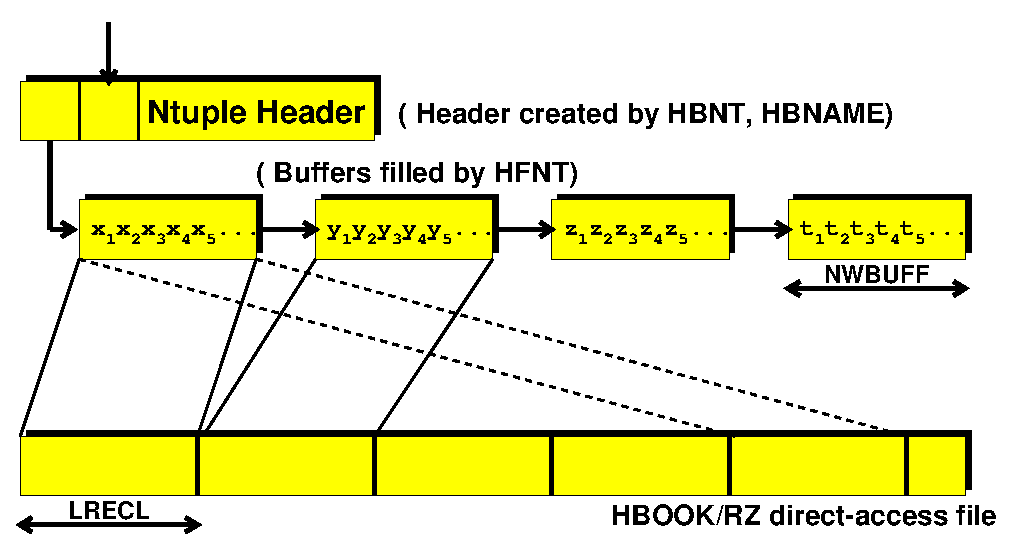
\epsfig{file=cwn.eps,width=.95\textwidth}}
\caption{Schematic structure of a CWN Ntuple}
\label{fig:cwn}
\newcommand{\III}{\(\sb{\mathtt{i}}\)}

\small

Figure~\ref{fig:cwn} shows the layout of a \CWN{} Ntuple.
The buffer size for each of the columns
\Lit{NWBUFF} was set equal to the record length \Rarg{LRECL}
(defined with routine \Rind{HROPEN}).
A \CWN{} requires a large value for the length of the common \Lit{/PAWC/},
\index{common {\tt/PAWC/}}\index{PAWC@{\tt/PAWC/} common}%
in any case larger than the number of columns
times the value \Lit{NWBUFF}, i.e. \Lit{NWPAWC>NWBUFF*NCOL}.
You can, however, expect important performance improvements by setting
the buffer size \Lit{NWBUFF} equal to a
multiple of the record length \Rarg{LRECL} (via routine \Rind{HBSET}).

In both figures, \Lit{x\III}, \Lit{y\III}, \Lit{z\III},
\Lit{t\III}, etc. represent the columns of event \Lit{i}.

\end{figure}
\clearpage
%end{latexonly}

\begin{htmlonly}
\begin{figure}
\begin{makeimage}
\includegraphics[width=\linewidth]{rwn.eps}
\end{makeimage}
\caption{Schematic structure of a RWN Ntuple}
\label{fig:rwn}
\end{figure}

\begin{figure}
\begin{makeimage}
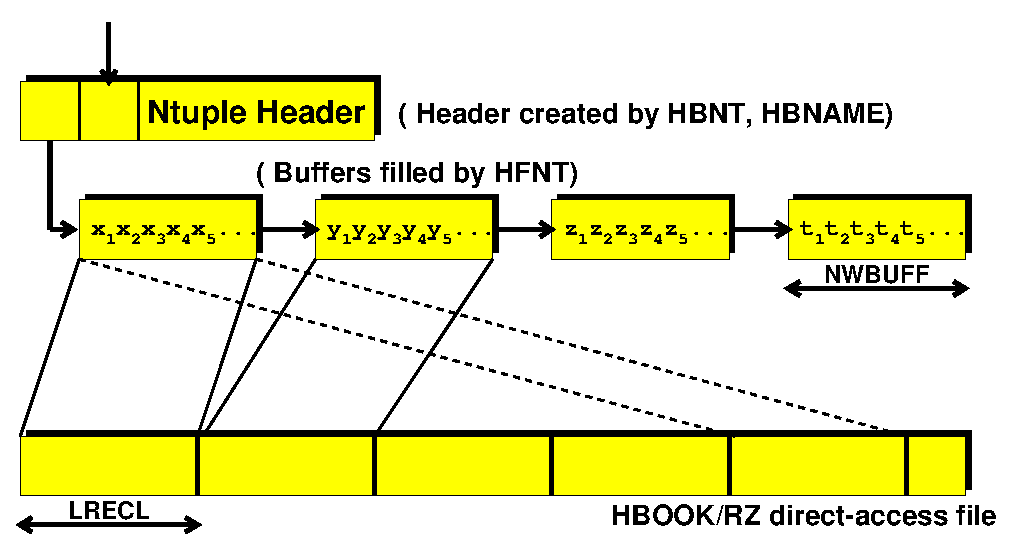
\includegraphics[width=\linewidth]{cwn.eps}
\end{makeimage}
\caption{Schematic structure of a CWN Ntuple}
\label{fig:cwn}
\end{figure}

\newcommand{\III}{\(\sb{\mathtt{i}}\)}

Figure~\ref{fig:cwn} shows the layout of a \CWN{} Ntuple.
The buffer size for each of the columns
\Lit{NWBUFF} was set equal to the record length \Rarg{LRECL}
(defined with routine \Rind{HROPEN}).
A \CWN{} requires a large value for the length of the common \Lit{/PAWC/},
in any case larger than the number of columns
times the value \Lit{NWBUFF}, i.e. \Lit{NWPAWC>NWBUFF*NCOL}.
You can, however, expect important performance improvements by setting
the buffer size \Lit{NWBUFF} equal to a
multiple of the record length \Rarg{LRECL} (via routine \Rind{HBSET}).

In both Figures \ref{fig:rwn} and \ref{fig:cwn}, \Lit{x\III},
\Lit{y\III}, \Lit{z\III}, \Lit{t\III}, etc., represent the columns of
event \Lit{i}.
\end{htmlonly}

\section{Row-Wise-Ntuples (RWN)}
\label{sec:NtupleRWN}
\subsection{Booking a RWN}
\label{HNTUBOOK}

\Shubr{HBOOKN}{(ID,CHTITL,NVAR,CHRZPA,NWBUFF,CHTAGS)}

\Action Books a \RWN{} in memory or with
automatic overflow on an \Lit{RZ} file.
Only single precision floating point numbers (\Lit{REAL*4} on
32 bit machines) can be stored, no data compression is provided.

\begin{DLttc}{123456}
\item[{\rm\bf Input parameters:}]
\item[ID] Identifier of the Ntuple.
\item[CHTITL] Character
    variable containing the title associated with the Ntuple.
\item[NVAR] Number of variables per event (\Lit{NVAR\(\leq\)512})
\item[CHRZPA] Character variable containing the path
    name of a RZ file onto which the contents of the Ntuple
    can overflow.
    \begin{DLttc}{123456}
    \item[' '] {\bf Memory resident Ntuples:} \\
    \index{Ntuple!memory resident}%
        A bank of \Lit{NWBUFF} words is created.
        Further banks of the same size are added in a linear
        chain should additional space be required at filling time.
    \item['RZTOP'] {\bf Disk resident Ntuples:} (recommended) \\
    \index{Ntuple!disk resident}%
        A disk resident Ntuple is created if the \Lit{CHRZPA}
        argument specifies the top directory name of an existing RZ file
        that has already been opened with \Rind{HROPEN} or \Rind{HRFILE}.
        A bank of length \Lit{NWBUFF} is created, as in the case of
        memory resident Ntuples. However, each time the bank becomes full
        it is automatically flushed to the RZ file, rather than
        creating additional banks in memory.
    \end{DLttc}
\item[NWBUFF]Number of words for the primary allocation for the Ntuple.
\item[CHTAGS] Character array of length \Lit{NVAR}, providing a short
    name (up to eight characters) tagging scheme for each variable.
\end{DLttc}

\begin{XMPt}{Example of the declaration of a memory resident RWN}
      CHARACTER*2 CHTAGS(5)
      DATA CHTAGS/'Px','Py','Pz','Q2','NU'/
 *
      CALL HBOOKN(10,'My first Ntuple',5,' ',1000,CHTAGS)
\end{XMPt}

\subsection{Filling a RWN}
\label{HNTUFILL}

\Shubr{HFN}{(ID,X)}

\Action
Fills a \RWN{}.

\begin{DLttc}{123456}
\item[{\rm\bf Input parameters:}]
\item[ID] Identifier of the Ntuple.
\item[X] Array of dimension \Lit{NVAR} containing
the values for the current event.
\end{DLttc}

\subsection*{Memory resident Ntuples}
\index{Ntuple!memory resident}

When a \RWN{} is booked, HBOOK reserves space in memory
in which to store the data, as specified by the \Rarg{NWBUFF}
argument of routine \Rind{HBOOKN}.
\index{memory}
As the \RWN{} is filled by a call to \Rind{HFN},
this space will be successively used until full.
At that time, a new memory allocation will be made
and the process continues.

If this data is then written to disk, it appears as one
enormous logical record.
In addition, it most cases the last block of data will
not be completely filled thus wasting space.

If one tries to reprocess this \RWN{} at a later date,
e.g. with \PAW{}, there must be enough space in memory to
store the entire Ntuple.
This often gives rise to problems
and so the following alternative method is recommended.

\subsection*{Circular buffer}
\index{circular buffer}

In an online environment you often want to have the last $N$ events
inside a buffer, so that the experiment can be monitored continuously.
To make it easier to handle this case, you can use routine \Rind{HFNOV},
which fills a circular buffer in memory with \RWN{} events, and when
the buffer is full, overwrites the oldest Ntuple.

\Shubr{HFNOV}{(ID,X)}

\Action
Fills a circular buffer with \RWN{}s.

\begin{DLttc}{123456}
\item[{\rm\bf Input parameters:}]
\item[ID] Identifier of the Ntuple.
\item[X] Array of dimension \Lit{NVAR} containing
the values for the current event.
\end{DLttc}

\subsection*{Disk resident Ntuples}
\index{Ntuple!disk resident}

Prior to booking the \RWN{}, a new HBOOK RZ file is created
using \Rind{HROPEN}.
The top directory name of this file is passed
to routine \Rind{HBOOKN} when the Ntuple is booked.

Filling proceeds as before but now, when the buffer in memory
is full, it is written to the HBOOK file and then reused
for the next elements of the Ntuple.
This normally results in a more efficient
utilisation of the memory,
both when the Ntuple is created and when it is reprocessed.

\begin{XMPt}{Recommended way of creating a RWN}
      PROGRAM TEST
      PARAMETER (NWPAWC = 15000)
      COMMON/PAWC/PAW(NWPAWC)
      CHARACTER*8 CHTAGS(5)
      DIMENSION EVENT(5)
      EQUIVALENCE (EVENT(1),X),(EVENT(2),Y),(EVENT(3),Z)
      EQUIVALENCE (EVENT(4),ENERGY),(EVENT(5),ELOSS)
      DATA CHTAGS/'X','Y','Z','Energy','Eloss'/
*
      CALL HLIMIT(NWPAWC)
      CALL HROPEN(1,'EXAMPLE','EXAMPLE.DAT','N',1024,ISTAT)
      IF(ISTAT.NE.0)GO TO 99
*
      CALL HBOOKN(10,'A Row-Wise-Ntuple',5,'//EXAMPLE',5000,CHTAGS)
      CALL HBOOK1(100,'Energy distribution',100,0.,100.,0.)
*
      DO 10 I=1,10000
         CALL RANNOR(X,Y)
         Z=SQRT(X*X+Y*Y)
         ENERGY=50. + 10.*X
         ELOSS=10.*ABS(Y)
         CALL HFN(10,EVENT)
         CALL HFILL(100,ENERGY,0.,1.)
 10   CONTINUE
*
      CALL HROUT(0,ICYCLE,' ')
      CALL HREND('EXAMPLE')
*
 99   CONTINUE
      END
\end{XMPt}

When the Ntuple is filled, routine \Rind{HFN} will automatically write
the buffer to the directory in the RZ~file, which was specified in the
call to \Rind{HBOOKN} (the top directory \Lit{//EXAMPLE} in the
example above).  If the current directory 
(CD)\index{current directory}\index{directory!current} is different,
\Rind{HFN} will save and later automatically restore the CD.

The Ntuple created by the program shown above can be processed
by \PAW{} as follows.

\begin{XMPt}{Reading an RWN in a PAW session}
            PAW > Histo/file  1  example.dat
            PAW > Histo/plot 100
            PAW > Ntuple/plot 10.energy
            PAW > Ntuple/plot 10.eloss  energy<50
            PAW > Ntuple/plot 10.eloss%energy  x<2.and.sqrt(z)>1
\end{XMPt}

By default \Rind{HROPEN} creates a file that can be extended up to
32000 blocks, i.e. 128 Mbytes for a record length \Lit{LREC}
of 1024 words.
If one wishes to create very large Ntuples, one should
make two changes to the above procedure.

\begin{UL}
\item A large value should be used for the record length of the file,
      e.g. 8192 words (the maximum on most machines).
      {\bf N.B. the maximum record length on VMS systems is 8191 words.
      If access mode \Lit{RELATIVE} is used, the maximum is 4095 words.}
      This remark does not apply to a \CWN, as described later.
\item Option \Lit{Q} on \Rind{HROPEN} should be used to override the default
      number of records allowed.
\end{UL}

This can be achieved as by changing the previous call to \Rind{HROPEN}
as follows:

\begin{XMPt}{Writing very large Ntuple files}
              COMMON/QUEST/IQUEST(100)
              CALL HLIMIT(150000)
*
*     Create HBOOK file with the maximum record length (32756 bytes)
*     and maximum number of records (65000)
*
              IQUEST(10) = 65000
              CALL HROPEN(1,'EXAMPLE','EXAMPLE.DAT','NQ',8192,ISTAT)
              IF(ISTAT.NE.0)GO TO 99
\end{XMPt}
\index{IQUEST@{\tt IQUEST} communication vector}

%\finalnewpage%%%%%%%%%%%%%%%%%%%%%%%%%%%%%%%%%%%%%%%%%%%%%%%%%%%%%%%%%%

\section{More general Ntuples: Column-Wise-Ntuples (CWN)}
\label{sec:NtupleCWN}

A \CWN{} supports the storage of the following data types: floating
point numbers (\Lit{REAL*4} and \Lit{REAL*8}), integers, bit patterns
(unsigned integers), booleans and character strings.

\subsection*{Data Compression}

Floating point numbers, integers and bit patterns can be packed by
specifying a range of values or by explicitly specifying the number
of bits that should be used to store the data. Booleans are always
stored using one bit. Unused trailing array elements will not be
stored when an array depends on an index variable. In that case only
as many array elements will be stored as specified by the index
variable.

For example, the array definition \Lit{NHITS(NTRACK)}
defines \Lit{NHITS} to depend on the index variable \Lit{NTRACK}.
When \Lit{NTRACK} is 16, the elements \Lit{NHITS(1..16)} are stored,
when \Lit{NTRACK} is 3, only the elements one to three
(\Lit{NHITS(1..3)}) are stored, etc.

\subsection*{Storage Model}

Column wise storage allows direct access to any column in the Ntuple.
Histogramming one column from a 300 column \CWN{} requires reading
only 1/300 of the total data set.
However, this storage scheme requires one memory buffer per column
as opposed to only one buffer in total for an \RWN.
By default the buffer length is 1024 words,
in which case a 100 column Ntuple requires 409600 bytes of buffer space.
In general, performance increases with buffer size.
Therefore, one should tune the buffer size (using routine \Rind{HBSET})
as a function of the number of columns and the amount of available memory.
Highest efficiency is obtained when setting the buffer size equal to the
record length of the RZ HBOOK file (as specified in the call to
\Rind{HROPEN}).
A further advantage of column wise storage is that a \CWN{}
can easily be extended with one or more new columns.

Columns are logically grouped into blocks (physically, however, all
columns are independent).
Blocks allow users to extend a \CWN{} with private columns or to
group relevant columns together.
New blocks can even be defined after a \CWN{} has been filled.
The newly created blocks can be filled using routine \Rind{HFNTB}.
For example, a given experiment might define a number of standard
Ntuples. These would be booked in a section of the code that
would not normally be touched by an individual physicist. However,
with a \CWN{} a user may easily add one or more blocks of information
as required for their particular analysis.

Note that arrays are treated as a single column.
This means that a \CWN{} will behave like a \RWN{},
with the addition of data typing and compression,
if only one array of \Lit{NVAR} elements is declared.
This is not recommended as one thereby loses
the direct column access capabilities of a \CWN{}.

\subsection*{Performance}

Accessing a relatively small number of the total number of
defined columns results in a huge increase in performance compared to
a \RWN{}.
However, reading a complete \CWN{} will take
slightly longer than reading a \RWN{} due to the overhead
introduced by the type checking and compression mechanisms and
because the data is not stored sequentially on disk.
The performance increase with a \CWN{} will most clearly show up when
using \PAW{}, where one typically histograms one
column with cuts on a few other columns.
The advantages of having different data types and data compression generally
outweighs the performance penalty incurred when reading a complete \CWN{}.

%\finalnewpage%%%%%%%%%%%%%%%%%%%%%%%%%%%%%%%%%%%%%%%%%%%%%%%%%%%%%%%%%%

\subsection{Booking a CWN}
\label{HNTUBOOKT}

The booking is performed in two stages.
Firstly, a call to \Rind{HBNT}
is made to declare the Ntuple identifier and title.
Secondly, one or more
calls are made to \Rind{HBNAME} or \Rind{HBNAMC} to describe
the variables that are to be stored in the Ntuple.
Routine \Rind{HBNAMC} is used to define \Lit{CHARACTER} variables,
while all other variable types are defined with routine \Rind{HBNAME}.

\Shubr{HBNT}{(ID,CHTITL,CHOPT)}

\Action
Books a \CWN.

\begin{DLttc}{12345678}
\item[{\rm\bf Input parameters:}]
\item[ID]     Identifier of the Ntuple.
\item[CHTITL] Character variable specifying the title associated to the Ntuple.
\item[CHOPT]  Character variable specifying the desired options.
   \begin{DLttc}{123}
     \item[' '] for disk resident Ntuples (default).
     \item['D'] idem as \Lit{' '}.
     \item['M'] for memory resident Ntuples.
   \end{DLttc}
\end{DLttc}

The CWN{} will be stored in the current HBOOK directory.
The variables to be stored in the Ntuple will be specified
with routine \Rind{HBNAME} or \Rind{HBNAMC} described below.

When the \CWN{} will be filled with \Rind{HFNT}, the memory buffers associated
with each column will be written to the file and directory corresponding
to the current working directory when \Rind{HBNT} was called.
Remember that when routine \Rind{HROPEN} is called, the current
working directory is automatically set to the
top directory of that file.
It is therefore convenient to call \Rind{HBNT} immediately after \Rind{HROPEN}.
If this was not the case, routine \Rind{HCDIR} must be called prior to
\Rind{HBNT} to set the current working directory.
When the Ntuple has been filled (via calls to \Rind{HFNT})
the resident buffers in memory as well as the Ntuple header
must be written to the file with a call to \Rind{HROUT}.
Before calling \Rind{HROUT}, the current working directory
must be set to the current directory when \Rind{HBNT} was called.

\Shubr{HBSET}{(CHOPT,IVAL,IERR*)}

\Action
Set global Ntuple options.

\begin{DLttc}{123456}
\item[{\rm\bf Input parameters:}]
\item[CHOPT] Character variable specifying the parameter to set.
   \begin{DLttc}{1234567}
     \item['BSIZE'] Set the buffer size. For each variable (i.e.\ column)
                    a buffer of \Lit{BSIZE} words is created in memory.
                    The default for \Lit{BSIZE} is 1024.
   \end{DLttc}
\item[IVAL]   Value for the parameter specified with \Rarg{CHOPT}.
\item[{\rm\bf Output parameters:}]
\item[IERR]   Error return code (\Lit{=0} means no errors).
\end{DLttc}

If the total memory in \Lit{/PAWC/},
\index{common {\tt/PAWC/}}\index{PAWC@{\tt/PAWC/} common}%
allocated via \Rind{HLIMIT}
is not sufficient to accomodate all the column buffers of \Rarg{BSIZE} words,
then \Rind{HBNT} will automatically reduce the buffer size in such a way that
 all buffers can fit into
memory.
It is strongly recommended to allocate enough memory to \Lit{/PAWC/}
in such a way that each column buffer is at least equal to the block size of
the file.
A simple rule of thumb in the case of no data compression is to have
\mbox{\Lit{NWPAWC>NCOL*LREC}}, where \Lit{NWPAWC}
is the total number of words allocated
by \Rind{HLIMIT}, \Lit{LREC} is the block size of the file in machine words
as given in the call to \Rind{HROPEN}  and \Lit{NCOL} is the number of columns.

%\finalnewpage%%%%%%%%%%%%%%%%%%%%%%%%%%%%%%%%%%%%%%%%%%%%%%%%%%%%%%%%%%

\subsection{Describing the columns of a CWN}
\label{HNTUDESC}

\Shubr{HBNAME}{(ID, CHBLOK, VARIABLE, CHFORM)}

\Shubr{HBNAMC}{(ID, CHBLOK, VARIABLE, CHFORM)}
\Action
Describe the variables to be stored in a \CWN{}
(non-character and character variables, respectively).

\begin{DLttc}{12345678}
\item[{\rm\bf Input parameters:}]
\item[ID]     Identifier of the Ntuple as in the call to \Rind{HBNT}.
\item[CHBLOK] Character variable of maximum length 8 characters
              specifying the name by which the block
              of variables described by \Lit{CHFORM} is identified.
\item[VARIABLE]
              The first variable that is described in \Lit{CHFORM}.
              Variables must be in common blocks but may not be
              in a ZEBRA bank.
              For example, given the common block \Lit{CEXAM} described
              below, one would call \Lit{HBNAME} with the argument \Lit{IEVENT}.
              In the case of character variables, the routine
              \Lit{HBNAMC} must be used. In all other cases one
              should use \Lit{HBNAME}.
\item[CHFORM] Can be either a character string describing the variables
              to be stored in block \Lit{CHBLOK} or:
   \begin{DLttc}{1234567}
     \item['\$CLEAR'] To clear the addresses of all variables in the Ntuple.
     \item['\$SET'] To set the addresses in which to write the values of
                    all variables in block \Lit{CHBLOK}.
   \end{DLttc}
             The last two forms are used before reading back the Ntuple data
             using \Rind{HGNT}, \Rind{HGNTB}, \Rind{HGNTV} or \Rind{HGNTF}.
             See also \Rind{HUWFUN}.
\end{DLttc}

With \Lit{CHFORM} the variables, their type, size and, possibly, range
(or packing bits) can all be specified at the same time.
{\bf Note however that variable names should be unique, even when
they are in different blocks}.

The routine \Rind{HNFORM} (see below) can be used to ease the task of
generating the \Lit{CHFORM} character string.

In the simplest
case \Lit{CHFORM} corresponds to the COMMON declaration. For example:
\begin{XMP}
       COMMON /CEXAM/ IEVENT, ISWIT(10), IFINIT(20), NEVENT, NRNDM(2)
\end{XMP}
can be described by the following \Lit{CHFORM}:
\begin{XMP}
       CHFORM = 'IEVENT, ISWIT(10), IFINIT(20), NEVENT, NRNDM(2)'
\end{XMP}
in this case the Fortran type conventions are followed and the default
sizes are taken. Note that to get a nice one-to-one
correspondance between the COMMON and the \Lit{CHFORM} statements
the dimensions of the variables are specified in the COMMON and not
in a DIMENSION statement.

The default type and size of a variable can be overridden by
extending the variable name with \Lit{:<t>*<s>}:

\begin{tabular}{@{}>{\tt}cllcl}
\Lit{<t>} & type of variable & \Lit{<s>} values & default & routine      \\[1mm]
 R        & floating-point   & 4, 8             & 4       & \Rind{HBNAME}\\
 I        & integer          & 4, 8             & 4       & \Rind{HBNAME}\\
 U        & unsigned integer & 4, 8             & 4       & \Rind{HBNAME}\\
 L        & logical          & 4                & 4       & \Rind{HBNAME}\\
 C        & character        & \tt[4$\le$s$\le$32] (multiple of 4)
                                                & 4       & \Rind{HBNAMC}\\
\end{tabular}

%\finalnewpage%%%%%%%%%%%%%%%%%%%%%%%%%%%%%%%%%%%%%%%%%%%%%%%%%%%%%%%%%%

\subsubsection{Packing variables in a CWN}
Significant data storage savings can be achieved in the Ntuple when the
range of a type \Lit{U}, \Lit{I} or \Lit{R} variable is known. In such cases
the number of bits required to store all possible values of the variable
is calculated by HBOOK, and the data suitably packed. For example, an integer
run number, \Lit{IRUN}, which takes values from 8000 to 8007 should be
specified as \Lit{IRUN[8000,8007]}, and HBOOK will automatically use
3 bits to store the
variable in the resulting Ntuple. By the same token, if the variable is
known to only require a certain number of bits, then this should also be
indicated in \Lit{CHFORM} by adding that number after the type specification
using \Lit{:<b>} for types \Lit{U}
and \Lit{I} and \Lit{:<b>:[<min>,<max>]} for type \Lit{R}. For example, if
\Lit{IRUN} takes values between 0 and 10, then the declaration should be
\Lit{IRUN:I*4:4} (4 bits are allocated). Note that the type declaration
simply describes how the variable is stored in memory when the HBOOK program
is run, and is not necessarily a description of its size in the resulting
Ntuple.

Floating-points are packed into an integer using:
\begin{XMP}
IPACK = ((R - <min>)/(<max> - <min>)*(2**<b> - 1) + 0.5
\end{XMP}

When the bit-packing specifier \Lit{:<b>...} is not given, HBOOK will store
the variable using the number of bytes given by \Lit{<s>} or the default (see
the table above for a list of defaults for each type).

In case the default type and size of a variable should be used, the
packing bits can be specified as \Lit{::<b>...}.

If the bit-packing specifier is given, then it must be in the range
\Lit{1}\(\le\)\Lit{b}\(\le\)\Lit{8*<s>}, where \Lit{<s>} either
appears in the \Lit{CHFORM} declaration, or is the assumed default.

Logical variables are always stored in 1 bit by HBOOK.

\subsubsection{Alignment of variables declared in \Lit{CHFORM}}
Variables declared in \Lit{CHFORM} must always be aligned on a word boundary.
In other words, all variables (including character strings) must be declared
in the calling program with alength that is a multiple of 4 bytes. Character
variable \textit{names} (not their contents) are limited to a maximum of 32
characters.

\subsubsection{Variable length Ntuple rows}
Variable-length Ntuple rows and looping over array components
are also supported to optimize Ntuple storage and Ntuple plotting.
Variable row length occurs when arrays in the Ntuple
depend on an index variable which varies.

\finalnewpage

\begin{XMPt}{Example of a variable row length CWN definition}
      PARAMETER (MAXTRK = 100, MAXHIT = 300)
      COMMON /CMTRK/ NTRACK, NHITS(MAXTRK), PX(MAXTRK), PY(MAXTRK),
     +               PZ(MAXTRK), XHITS(MAXHIT,MAXTRK), YHITS(MAXHIT,MAXTRK),
     +               ZHITS(MAXHIT,MAXTRK)
      CALL HBNAME(ID,'VARBLOK2',NTRACK,
     +            'NTRACK[0,100], NHITS(NTRACK)[0,300],'//
     +            'PX(NTRACK), PY(NTRACK), PZ(NTRACK), XHITS(300,NTRACK),'//
     +            'YHITS(300,NTRACK), ZHITS(300,NTRACK)')
\end{XMPt}

In this example the number of elements to store in one Ntuple row
depends on the number of tracks, \Lit{NTRACK}.
The call to \Rind{HBNAME} declares \Lit{NTRACK} to be an
index variable and that the size of the Ntuple row depends on the value of
this index variable.

\subsubsection{Ranges of index variables in a CWN}
The range of an index variable is specified using \Lit{[<l>,<u>]},
where \Lit{<l>} is the lower and \Lit{<u>} the upper limit of the arrays
using this index variable. In the above example the
lower limit of \Lit{NTRACK} is 0 and the upper limit is 100 (\Lit{= MAXTRK}).
While filling a \CWN{} HBOOK can also easily test for
array out-of-bound errors since it knows the range of \Lit{NTRACK}.

Only the last dimension of a multi-dimensional array may be variable
and the index variable must be specified in the block where it is used.
Array lower bounds must, just like the lower range of the index variable,
be 0.

\subsubsection{Multiple calls to \Lit{HBNAME}}
\Rind{HBNAME} may be called more than once per block as long as no data
has been stored in the block.
New blocks can be added to an Ntuple at any time, even after filling has
 started,
whereas existing blocks may only be extended before filling has started.
\index{block}

\subsection{Creating \texttt{CHFORM} dynamically}

\Shubr{HNFORM}{(CHFORM,CHNAME,LDIM,CHTYPE,XLOW,XHIGH)}

\Action Assists with the formation of the character string \Lit{CHFORM}.

\begin{DLttc}{123456}
\item[{\rm\bf Input parameters:}]
\item[CHFORM] The character string to be started or appended to. The
  string should be declared of sufficient length in the calling
  routine such that it can hold the fully expanded specifications of
  the Ntuple variables.
\item[CHNAME] Character variable specifying the name of the variable
  to be added to \Lit{CHFORM}.  If the variable is dimensioned then
  \Lit{CHNAME} should contain the dimension specification in brackets,
  as usual. For dimension spcifications that are to be computed at run
  time, the \Lit{LDIM} argument is used, and a \Lit{*} used as a
  placeholder in the dimension specification for replacement by
  \Rind{HNFORM} at run time. See the examples.
\item[LDIM] Dimension(s) of the variable.  If the variable in
  \Lit{CHNAME} is not dimensioned, or its dimensions are hard-coded in
  \Lit{CHNAME}, then \Lit{LDIM} should be set to 0.  If there is one
  \Lit{*} placeholder in the dimension specification in \Lit{CHNAME}
  then \Lit{LDIM} should be set to the value of that dimension. For
  more than one placeholder, \Lit{LDIM} should be an integer array of
  appropriate size. See the examples.
\item[CHTYPE] A character variable specifying the type and bit-packing
  to be used for the variable in \Lit{CHNAME}. Possible values for the
  type are \Lit{[R,I,U,L,C][*[4..32]]}. The bit-packing number should
  appear after a ":".
\item[XLOW] The lowest value that the variable in \Lit{CHNAME} may
  take. This may be specified as either a real or integer value.
\item[XHIGH] The highest value that the variable in \Lit{CHNAME} may
  take.  If \Lit{XHIGH} is less than or equal to \Lit{XLOW}, then no
  limits will be encoded by \Lit{CHFORM}.
\end{DLttc}

The following example shows how \Lit{HNFORM} may be used to aid the
creation of an Ntuple:

\begin{XMPt}{Example of booking an Ntuple with \Rind{HNFORM} and \Rind{HBNAME}}
      PARAMETER (MAXTRK = 100, MAXHIT = 300)
      COMMON /CMTRK/ NTRACK, NHITS(MAXTRK), PX(MAXTRK), PY(MAXTRK),
     +               PZ(MAXTRK), XHITS(MAXHIT,MAXTRK), YHITS(MAXHIT,MAXTRK),
     +               ZHITS(MAXHIT,MAXTRK)
      CHARACTER*500 CHFORM

      CHFORM(:) = ' '
      CALL HNFORM(CHFORM,'NTRACK',0,' ',0.,REAL(MAXTRK))
      CALL HNFORM(CHFORM,'NHITS(NTRACK)',0,' ',0.,REAL(MAXHIT))
      CALL HNFORM(CHFORM,'PX(NTRACK)',0,' ',0.,0.)
      CALL HNFORM(CHFORM,'PY(NTRACK)',0,' ',0.,0.)
      CALL HNFORM(CHFORM,'PZ(NTRACK)',0,' ',0.,0.)
      CALL HNFORM(CHFORM,'XHITS(*,NTRACK)',MAXHIT,' ',0.,0.)
      CALL HNFORM(CHFORM,'YHITS(*,NTRACK)',MAXHIT,' ',0.,0.)
      CALL HNFORM(CHFORM,'ZHITS(*,NTRACK)',MAXHIT,' ',0.,0.)

      LFORM = INDEX(CHFORM,' ')-1

      CALL HBNAME(ID,'VARBLOK2',NTRACK,CHFORM(:LFORM))

\end{XMPt}





\subsection*{Alternative way of booking a CWN}

\Shubr{HBOOKNC}{(ID,CHTITL,NVAR,BLOCK,TUPLE,CHTAGS)}

\Action Provides a way to define a \CWN{} similar to
\Rind{HBOOKN} for a \RWN{}.

\begin{DLttc}{123456}
\item[{\rm\bf Input parameters:}]
\item[ID] Identifier of the CWN{}.
          If it does not already exist, it is created.
\item[CHTITL] Character variable specifying the name of the Ntuple
          (not used if it already exists).
\item[NVAR]  Number of variables per event (maximum 200).
\item[BLOCK] Name of the block inside the \CWN (default is \Lit{'Block1'}.
\item[TUPLE] Array of dimension \Lit{NVAR} that will contain values at filling
                 time.
\item[CHTAGS] Character array of length \Lit{NVAR}, providing a short
    name (up to eight characters) tagging scheme for each variable.
\end{DLttc}

\subsection{Filling a CWN}
\label{HNTUFILLT}

\Shubr{HFNT}{(ID)}

\Action Fill a \CWN{}.

\begin{DLttc}{123456}
\item[{\rm\bf Input parameter:}]
\item[ID] Identifier of the CWN{}.
\end{DLttc}
\Rind[HROPEN]{}
\Rind[HBNT]{}
\Rind[HBNAME]{}
\Rind[HBNAMC]{}
\Rind[HFNT]{}
\Rind[HROUT]{}
\Rind[HREND]{}
\index{PAW}


\Shubr{HFNTB}{(ID,CHBLOK)}

\Action Fill the named block \Lit{CHBLOK} in a \CWN{}.

\begin{DLttc}{123456}
\item[{\rm\bf Input parameters:}]
\item[ID] Identifier of the Ntuple.
\item[CHBLOK]Character variable specifying the block that is to be filled.
\end{DLttc}

\Shubr{HPRNT}{(ID)}

\Action Print the  definition of the CWN{} \Lit{ID} as
defined by the calls to \Rind{HBNAME} and/or \Rind{HBNAMC}.

\begin{DLttc}{123456}
\item[{\rm\bf Input parameter:}]
\item[ID] Identifier of the CWN{}.
\end{DLttc}

\subsection*{Recovery procedure}
\label{sec:Ntuple-recovery}

The Ntuple header, containing the essential
definitions associated with an Ntuple,
are now written to the output file when the first
buffer is written.
If the job producing the Ntuple does not terminate in a clean way
(i.e. the job crashs or you forgot to call \Rind{HROUT}),
it is now possible to rebuild the Ntuple header from the
information available in the file.
Note, however, that the events corresponding to the last
Ntuple buffer in memory are lost.

\Shubr{HRECOV}{(ID,CHOPT)}

\Action Recover the information associated with a \CWN{}.

\begin{DLttc}{123456}
\item[{\rm\bf Input parameters:}]
\item[ID]    Identifier of the CWN{}.
\item[CHOPT] Character variable specifying the option desired.
             At present Not used at present; \Lit{' '}
             should be specified
\end{DLttc}

%\finalnewpage%%%%%%%%%%%%%%%%%%%%%%%%%%%%%%%%%%%%%%%%%%%%%%%%%%%%%more com

\begin{XMPt}{Example of saving contents of common variables in an Ntuple}
        COMMON/GCFLAG/IDEBUG,IDEMIN,IDEMAX,ITEST,IDRUN,IDEVT,IEORUN
       +        ,IEOTRI,IEVENT,ISWIT(10),IFINIT(20),NEVENT,NRNDM(2)

        COMMON/GCTRAK/VECT(7),GETOT,GEKIN,VOUT(7),NMEC,LMEC(MAXMEC)
       + ,NAMEC(MAXMEC),NSTEP ,MAXNST,DESTEP,DESTEL,SAFETY,SLENG
       + ,STEP  ,SNEXT ,SFIELD,TOFG  ,GEKRAT,UPWGHT,IGNEXT,INWVOL
       + ,ISTOP ,IGAUTO,IEKBIN, ILOSL, IMULL,INGOTO,NLDOWN,NLEVIN
       + ,NLVSAV,ISTORY

        COMMON/GCTMED/NUMED,NATMED(5),ISVOL,IFIELD,FIELDM,TMAXFD,DMAXMS
       +      ,DEEMAX,EPSIL,STMIN,CFIELD,PREC,IUPD,ISTPAR,NUMOLD

        CHARACTER*4 TYPE
        COMMON/CMCC/TYPE

*     The code to book and fill the Ntuple would look like this:
*
*   Initialisation phase.
*   The calls to HROPEN, HBNT and HBNAME may be placed in different
*   initialisation routines.
*   In this example example the Ntuple will be stored in directory //MYFILE.
*
        CALL HROPEN(1,'MYFILE','geant.ntup','N',1024,ISTAT)
        CALL HBNT(10,'Geant Ntuple',' ')
*
        CALL HBNAME(10, 'RUN',    IDRUN,  'IDRUN::16,IDEVT::16')
        CALL HBNAME(10, 'RUN',    IEORUN, 'IEORUN::16')
        CALL HBNAME(10, 'VECT',   VECT,   'VECT(6)')
        CALL HBNAME(10, 'GEKIN',  GEKIN,  'GEKIN')
        CALL HBNAME(10, 'INWVOL', INWVOL, 'INWVOL[1,7],ISTOP[1,7]')
        CALL HBNAME(10, 'NUMED',  NUMED,  'NUMED::10')
        CALL HBNAME(10, 'NSTEP',  NSTEP,  'NSTEP::16')
        CALL HBNAMC(10, 'TYPE',   TYPE,   'TYPE:C')
*
*    To fill the Ntuple, when the common blocks are filled just invoke
*    routine HFNT which knows the addresses and the number of variables.
*
        DO 10 I = 1, 1000000
           ...
           CALL HFNT(10)
10      CONTINUE
*
*                      At the end of the job, proceed as usual
*
        CALL HROUT(10, ICYCLE, ' ')
        CALL HREND('MYFILE')

\end{XMPt}

%\finalnewpage%%%%%%%%%%%%%%%%%%%%%%%%%%%%%%%%%%%%%%%%%%%%%%

\subsection*{Disk resident Ntuples}

Histograms are never created directly on a disk file.
They are always created in the current directory in memory
(\Lit{//PAWC} or \Lit{//PAWC/subdir}).
Histograms are saved on the disk file with a call of type
\Lit{CALL \Rind{HROUT}}
In case of disk-resident Ntuples, it is the same thing.
The Ntuple header
(data structure containing the column names) is always created
in the current directory in memory
(\Lit{//PAWC} or \Lit{//PAWC/subdir}).
However, the call to \Rind{HBNT} remembers the current
directory on disk (in the case below
the \Lit{CD} on disk is \Lit{//K0}).
When you fill the Ntuple, \Rind{HFNT} fills a buffer in memory.
When this buffer is full, \Rind{HFNT} knows what is the \Lit{CD} on disk.
The buffer is written into that directory.
Note that your current directory on disk may be somewhere else.
\Rind{HFNT} will temporarely change the \Lit{CD} to \Lit{//K0}
and will reset the \Lit{CD} to what it was before calling \Rind{HFNT}.
At the end of your job, you have to save the header and the current buffer
in memory on the disk file.
For that you have to:

\begin{UL}
\item[--] Change the directory in memory where you book the Ntuple.
          If you do not have subdirectories,
          this operation is not necessary.
\item[--] Change the directory on disk where you specified it in
          \Rind{HBNT}.
          In the case below \Lit{//KO}.
\item[--] Issue a call to \Rind{HROUT} or \Rind{HREND}.
\end{UL}

\begin{XMPt}{Creating a disk resident Ntuple}
      call HCDIR('//PAWC',' ')
*--     HROPEN sets the directory to //K0, so no call to HCDIR is needed
      call HROPEN(50,'K0','~/mydir/K0.rz','N',1024,ISTAT)
      if (ISTAT.ne.0) write(6,*) 'Error in HROPEN'
      call HBNT(1000,'Ntuple','D')
      call HLDIR('//PAWC','T') ! Now you can see the header in //PAWC
      call HLDIR('//K0','T')   ! OK, nothing yet on //K0
*--     HBNAME describes the Ntuple
      call HBNAME(1000,'Event',EvtNo,
     +            'RunNo:I,Evtno:I,NPos:I,NNeg:I,'//
     +            ....
....
        call HLDIR('//K0','T') ! Nothing yet on //K0
        call HCDIR('//K0',' ') ! Useless, HFNT remembers that buffers are
 written to //KO
        call HFNT(1000)
        call HLDIR(' ','T')    ! This will not show anything on //K0.
                               ! However if you call HLDIR(' ','TA') you will
 see all Ntuple
                               ! extensions in the case you have many calls to
 HFNT.
                               ! In this particular example everything is still
 in memory.
....
      call HCDIR('//K0',' ')   ! Useless, you are already here
      call HLDIR('//K0',' ')   ! same as call hldir(' ','T')
      call RZLDIR(' ',' ')
      call HROUT(0,icycle,' ')
*-*      If you call HLDIR(' ',' ') here you will see the header
*-*      If you call HLDIR(' ','A') here you will see the header and your Ntuple
 extensions
      call HREND('K0')
\end{XMPt}

\finalnewpage%%%%%%%%%%%%%%%%%%%%%%%%%%%%%%%%%%%%%%%%%%%%%%

\section{Making projections of a RWN}
\label{HNTUPROJ}

\Shubr{HPROJ1}{(ID,IDN,ISEL,FUN,IFROM,ITO,IVARX)}

\Action
Fill an existing one-dimensional histogram with data from a RWN.

\begin{DLttc}{123456}
\item[{\rm\bf Input parameters:}]
\item[ID]    Identifier of 1-dimensional histogram, which
             must have been previously booked with \Rind{HBOOK1}.
\item[IDN]   Identifier of the RWN Ntuple.
\item[ISEL]  Selection flag
             \begin{DLttc}{123}
                \item[0]   No selection criterion.
                           Events between \Lit{IFROM} and
                           \Lit{ITO} histogrammed with weight one.
                \item[<>0] Function \Lit{FUN} is called for each event
                           between \Lit{IFROM} and \Lit{ITP};
                           they are histogrammed
                           with a weight equal to the value of \Lit{FUN}.
             \end{DLttc}
\item[FUN]   User function, to be declared \Lit{EXTERNAL} in the calling
             routine.
             It has as parameters the array of variables \Lit{X} and the
             selection flag \Lit{ISEL}. If \Lit{FUN=0.},
             no filling takes place for that event.
\item[IFROM] Event number where the histogramming has to start.
\item[ITO]   Event number where the histogramming has to end.
\item[IVARX] Sequence number in the Ntuple of the variable to be
             histogrammed.
\end{DLttc}

\begin{XMPt}{Example of the use of a one-dimensional Ntuple projection}
     PROGRAM MAIN
     EXTERNAL WFUNC
     CALL HPROJ1(10,20,1,WFUNC,0,0,4)
     .....
     FUNCTION WFUNC(X,ISEL)
     DIMENSION X(*)
     WFUNC=0.
     IF(ISEL.EQ.1)     THEN
              IF(X(2)**2 +X(3)**2.LT.0.)WFUNC=1.
     ELSEIF(ISEL.EQ.2) THEN
              IF(X(2)**2 +X(3)**2.GT.5.)WFUNC=1.
     ELSE     WFUNC=X(5)
     ENDIF
     END
\end{XMPt}

\finalnewpage

Note that in an interactive session with \PAW{},
the user function \Lit{FUN} can be defined
interactively using a Fortran-like syntax without recompilation
and relinking.

\Shubr{HPROJ2}{(ID,IDN,ISEL,FUN,IFROM,ITO,IVARX,IVARY)}

\Action
Same action as \Rind{HPROJ1}, but filling a previously
booked 2-dimensional histogram or a profile histogram.
Variable \Lit{X(IVARX)} will be projected onto the \Lit{X} axis and
\Lit{X(IVARY)} onto the \Lit{Y} axis for all entries in the Ntuple
between \Lit{IFROM} and \Lit{ITO} inclusive.

The number of entries in an Ntuple can be obtained by \Rind{HNOENT}.

%\finalnewpage%%%%%%%%%%%%%%%%%%%%%%%%%%%%%%%%%%%%%%%%%%%%%%%%%%%%%%%%%%%%%%%

\section{Get information about an Ntuple}

\Shubr{HGIVEN}{(ID,CHTITL*,*NVAR*,CHTAG*,RLOW*,RHIGH*)}

\Action
Routine to provide information about an Ntuple.

\begin{DLttc}{123456}
\item[{\rm\bf Input parameters:}]
\item[ID] Identifier of the Ntuple.
\item[NVAR] Dimension of arrays \Lit{TAGS}, \Lit{RLOW}
and \Lit{RHIGH}.
\item[{\rm\bf Output parameters:}]
\item[CHTITL] Character
variable containing the title associated with the Ntuple.
\item[NVAR] The original contents is overwritten by the actual dimension of the
 Ntuple.
If \Lit{ID1} does not exist or is not an Ntuple \Lit{NVAR=0} is returned.
\item[CHTAG] Character array of dimension \Lit{NVAR}, which
contains the tag names of the Ntuple elements.
\item[RLOW] Array of dimension \Lit{NVAR}, which
contains the lowest value for each Ntuple element.
\item[RHIGH] Array of dimension \Lit{NVAR}, which
contains the highest value for each Ntuple element.
\end{DLttc}

\subsection{Retrieve the contents of a RWN into an array}

\Shubr{HGN}{(ID,*IDN*,IDNEVT,X*,IERROR*)}

\Action
Copy the contents of a \RWN{} event into an array.

\begin{DLttc}{123456}
\item[{\rm\bf Input parameters:}]
\item[ID]     Identifier of the Ntuple.
\item[IDN]    Must be initialized to zero before the first call to \Rind{HGN}.
\item[IDNEVT] Event number
\item[{\rm\bf Output parameters:}]
\item[IDN]    Internal HBOOK pointer
\item[X]      Array to contain variables for the event chosen.
\item[IERROR] Error return code.
\end{DLttc}

This routine returns in the vector \Lit{X} the contents of the
row \Lit{IDNEVT} or Ntuple \Lit{ID}.
The vector \Lit{X} must be of size \Lit{NVAR},
as specified in the call to \Rind{HBOOKN}.
If more than one row of the Ntuple is to be processed, it is more
efficient to call first \Rind{HGNPAR} and then \Rind{HGNF}.

\Shubr{HGNPAR}{(ID,CHROUT)}

\Action
Obtains the address and parameters of Ntuple ID.
\begin{DLttc}{123456}
\item[{\rm\bf Input parameters:}]
\item[ID]Identifier of the Ntuple.
\item[CHROUT]Character variable containing the name of the calling
subroutine (printed in case of errors).
\end{DLttc}

This routine sets some internal pointers and must be called before
the first call to \Rind{HGNF} for a given \RWN{}. When accessing
more than one row of an Ntuple it is more efficient to call
\Rind{HGNPAR} and then \Rind{HGNF} for each row that is required
than to call \Rind{HGN}.

\Shubr{HGNF}{(ID,IDNEVT,X*,IERROR*)}

\Action
Copy the contents of an Ntuple event into an array.
The routine \Rind{HGNPAR} must have been called
prior to the first call to \Rind{HGNF} for a given
Ntuple.

\begin{DLttc}{123456}
\item[{\rm\bf Input parameters:}]
\item[ID]Identifier of the Ntuple.
\item[IDNEVT]Event number
\item[{\rm\bf Output parameters:}]
\item[X] Array to contain variables for the event chosen.
\item[IERROR] Error return code.
\end{DLttc}

This routine returns in the vector \Lit{X} the contents of the
row \Lit{IDNEVT} or Ntuple \Lit{ID}.
The vector \Lit{X} must have be of size \Lit{NVAR},
as specified in the call to \Rind{HBOOKN}.

\begin{XMPt}{Example of access to RWN information}
\baselineskip=.95\baselineskip\relax      PROGRAM TEST
      INTEGER    NWPAWC
      PARAMETER (NWPAWC=15000, MTUPLE=5)
      COMMON/PAWC/PAW(NWPAWC)
      CHARACTER*80 CHTITL
      CHARACTER*8 CHTAGS(MTUPLE),CHTAGZ(MTUPLE)
      DIMENSION EVENT(MTUPLE),RLOW(MTUPLE),RHIGH(MTUPLE)
      EQUIVALENCE (EVENT(1),X),(EVENT(2),Y),(EVENT(3),Z)
      EQUIVALENCE (EVENT(4),ENERGY),(EVENT(5),ELOSS)
      DATA CHTAGS/'X','Y','Z','Energy','Eloss'/
*-- Tell HBOOK how many words are in PAWC.
      CALL HLIMIT(NWPAWC)
*-- Book Ntuple
      CALL HBOOKN(10,'A Row-Wise-Ntuple',5,' ',5000,CHTAGS)
*-- Fill the Ntuple
      DO 10 I=1,1000
         CALL RANNOR(X,Y)
         Z=SQRT(X*X+Y*Y)
         ENERGY=50. + 10.*X
         ELOSS=10.*ABS(Y)
         CALL HFN(10,EVENT)
 10   CONTINUE
*--   Obtain the definitions of the Ntuple
      NVAR = MTUPLE
      CALL HGIVEN(10,CHTITL,NVAR,CHTAGZ,RLOW,RHIGH)
      PRINT *,'Definitions of Ntuple # ',10
      PRINT *,'   Title: ',CHTITL(1:LENOCC(CHTITL))
      PRINT *,'   Number of variables: ',NVAR
      DO 20 I=1,NVAR
         PRINT 9001,I,RLOW(I),RHIGH(I)
9001  FORMAT(' Min/Max values for column # ',I3,1X,F10.5,
     +       1X,F10.5)
 20   CONTINUE
*--   Get the contents of 'event' # 333
      CALL HGNPAR(10,'TEST')
      CALL HGNF(10,333,EVENT,IERR)
      PRINT *,IERR,EVENT
*--   Get the number of events in this Ntuple
      CALL HNOENT(10,NEVENT)
      PRINT *,NEVENT
 99   CONTINUE
      END
\end{XMPt}

%\finalnewpage%%%%%%%%%%%%%%%%%%%%%%%%%%%%%%%%%%%%%%%%%%%%%%%%%%%%%%%%%%

\subsection{Retrieve the contents of a CWN into a common block}

\Shubr{HGNT}{(ID,IDNEVT,IERR*)}

\Action

Retrieve information about a \CWN{} row.

\begin{DLttc}{123456}
\item[{\rm\bf Input parameters:}]
\item[ID] Identifier of the Ntuple.
\item[IDNEVT] Number of the event about which information is required.
\item[{\rm\bf Output parameter:}]
\item[IERR] Error return code (\Lit{=0} if event was found)
\end{DLttc}

The information is restored at the addresses specified by \Rind{HBNAME}
or \Rind{HBNAMC} (for \Lit{CHARACTER} data).
If the information is being retrieved by a program other than the
one that wrote the Ntuple then \Rind{HBNAME}
or \Rind{HBNAMC} must be called as appropriate (see below).
\begin{XMP}
      CALL HBNAME(ID,' ',0,'$CLEAR')
      CALL HBNAME(ID,CHBLOK,VARIABLE,'$SET')
\end{XMP}
\Rind[HBNAME]{}
\Rind[HBNAMC]{}
These calls are required as \Lit{HBOOK} must obtain the location
at which the requested information is to be returned which is
obviously not valid between programs.
The first call clears all the addresses stored by \Lit{HBOOK}
for the specified Ntuple and the second one sets the
addresses for the variables in block \Lit{CHBLOK} starting at variable
\Lit{VARIABLE}. The second call should be repeated for every block of
which data has to be retrieved. The routine \Rind{HUWFUN} will generate
these calls automatically in the skeleton user function.

\Shubr{HGNTB}{(ID,CHBLOK,IROW,IERR*)}

\Action

Retrieve information about a named block in an Ntuple row.

\begin{DLttc}{123456}
\item[{\rm\bf Input parameters:}]
\item[ID] Identifier of the Ntuple.
\item[CHBLOK]Character variable specifying the block that is to be
retrieved.
\item[IROW] Number of the row about which information is required.
\item[{\rm\bf Output parameter:}]
\item[IERR] Error return code (\Lit{=0} if row was found)
\end{DLttc}

The information is restored at the addresses specified by \Rind{HBNAME}
or \Rind{HBNAMC} (for \Lit{CHARACTER} data).

\Shubr{HGNTV}{(ID,CHVAR,NVAR,IROW,IERR*)}

\Action

Retrieve information about the named variables in an Ntuple row.

\begin{DLttc}{123456}
\item[{\rm\bf Input parameters:}]
\item[ID] Identifier of the Ntuple.
\item[CHVAR] Array of character variables specifying the variables
             that are to be retrieved.
\item[NVAR]  Number of character variables specified in \Lit{CHVAR}.
\item[IROW] Number of the row about which information is required.
%\finalnewpage%%%%%%%%%%%%%%%%%%%%%%%%%%%%%%%%%%%%%%%%%%%%%%%%%%%%%%%%%%%%%%%%
\item[{\rm\bf Output parameter:}]
\item[IERR] Error return code (\Lit{=0} if row was found)
\end{DLttc}

The information is restored at the addresses specified by \Rind{HBNAME}
or \Rind{HBNAMC} (for \Lit{CHARACTER} data).

You should only call \Rind{HBNAME} for the blocks that
contain variables you want to read using \Rind{HGNTV}.
If you call \Rind{HBNAME} for all blocks you should
have a \Lit{PAWC} which is at least the same size as the one you used to
create the Ntuple.
If not you will run out of memory.

Also changing the buffer size will not help because the buffer used for
reading will be the same size as the buffer used to write the Ntuple.

There is a special option in \Rind{HBNAME} with which you can tell
\Rind{HBNAME} to only set the address
for a single variable in a block (this option
is used by PAW to reduce memory usage).

To set the address for a single variable call
\Rind{HBNAME} (or \Rind{HBNAMC}) as follows:
\begin{XMP}
      CALL HBNAME(ID, BLOCK, IADDR, '$SET:NTVAR')
\end{XMP}
This will tell \Rind{HGNTV} to restore the Ntuple
variable \Lit{NTVAR} in address \Lit{IADDR}.
Using this form of \Rind{HBNAME} will only reserve buffer space for
the variables you plan to read and not for all variables in the block.
However, you have to be careful that when you change the list
of variable for
\Rind{HGNTV} to also add or remove the correct \Rind{HBNAME} calls.

\Shubr{HGNTF}{(ID,IROW,IERR*)}

\Action

Retrieve information about all variables specified in a previous
call to either \Rind{HGNT}, \Rind{HGNTB} or \Rind{HGNTV}, in an Ntuple row.
This routine is much faster than either \Rind{HGNT}, \Rind{HGNTB} or
\Rind{HGNTV}.

\begin{DLttc}{123456}
\item[{\rm\bf Input parameters:}]
\item[ID] Identifier of the Ntuple.
\item[IROW] Number of the row about which information is required.
\item[{\rm\bf Output parameter:}]
\item[IERR] Error return code (\Lit{=0} if row was found)
\end{DLttc}

The information is restored at the addresses specified by \Rind{HBNAME}
or \Rind{HBNAMC} (for \Lit{CHARACTER} data).

\Shubr{HNTVDEF}{(ID1,IVAR,CHTAG,BLOCK,ITYPE)}

\Action

Returns the definition as given in \Rind{HBNAME} for
the variable with index \Lit{IVAR} in Ntuple \Lit{ID1}.
The Ntuple must already be in memory.

%\finalnewpage%%%%%%%%%%%%%%%%%%%%%%%%%%%%%%%%%%%%%%%%%%%%%%%%%%%%%%%%%%%%%

\subsection{Generate a user function}
\label{sec:userfunction}

HBOOK can automatically produce a skeleton user selection
function, which includes the Ntuple declaration via
the calls \Rind{HBNT}, \Rind{HBNAME} and \Rind{HBNAMC},
and can be used in a later run to access the elements of
the Ntuple.
Two cases are available; one for use in batch and the other for use with
\PAW.
In the first case the common block names will be those
specifed by the user in the call to \Rind{HBNAME} or \Rind{HBNAMC}.
For \PAW{}, these common names are
\Lit{/PAWCR4/}, \Lit{/PAWCR8/} and \Lit{/PAWCCH/} for storing
the ``single precision'' (\Lit{LOGICAL}, \Lit{INTEGER} and \Lit{REAL*4}),
``double precision'' (\Lit{REAL*8} and \Lit{COMPLEX}) and
\Lit{CHARACTER} data respectively.

\Shubr{HUWFUN}{(LUN,ID,CHFUN,ITRUNC,CHOPT)}

\Action

Write an user function or subroutine to access an Ntuple.

\begin{DLttc}{123456}
\item[{\rm\bf Input parameters:}]
\item[LUN] Logical unit used to write the user routine.
           \Lit{LUN} must be opened before this call.
\item[ID] Identifier of the Ntuple.
\item[CHFUN] Character variable specifying the routine name.
\item[ITRUNC] All variable names will be truncated to \Lit{ITRUNC}
              characters. \Lit{ITRUNC=0} is no truncation.
\item[CHOPT]  Character variable specifying the desired options.
   \begin{DLttc}{1234}
     \item['B'] Make an user subroutine for batch usage (i.e.
                with \Rind{HBNAME} and \Rind{HBNAMC} calls) (default).
     \item['P'] Make a \PAW{} selection function.
   \end{DLttc}
\end{DLttc}

A simple example of the two kinds of skeletons generated with
routine \Rind{HUWFUN} is given below.
Another more complex example can be found on page \pageref{sec:staffskeleton},
where the code of a fully worked out subroutine based on such
a sketeton can also be studied.

In \PAW{}, the command \Lit{UWFUNC} generates a skeleton for the
\RWN{} or \CWN{} analysis function automatically.

%\finalnewpage %%%%%%%%%%%%%%%%%%%%%%%%%%%%%%%%%%%%%%%%%%%%%%%%%%%%%%%%%%%%

\begin{XMPt}{Example of an Ntuple definition and HUWFUN usage}
      COMMON /CVECT/ V1, V2, V3, V4, V5, V6, V7, V8, V9, V10,
     +               V11, V12, V13, V14, V15, V16, V17, V18, V19, V20
      ...
      ...
*
*-- book N-tuple 20
*
      CALL HBNT(20,'1 block 20 variable N-tuple', ' ')
      CALL HBNAME(20,'VECT',V1,'V1,V2,V3,V4,V5,V6,V7,V8,V9,V10,V11,
     +                          V12,V13,V14,V15,V16,V17,V18,V19,V20')
*
      ...
      OPEN(11,FILE='nt20.f',STATUS='UNKNOWN')
      OPEN(12,FILE='nt20p.f',STATUS='UNKNOWN')
      CALL HUWFUN(11, 20, 'NT20', 0, 'B')
      CALL HUWFUN(12, 20, 'NT20', 0, 'P')
      ...
\end{XMPt}
The \Rind{HUWFUN} output files \Lit{nt20.f} and \Lit{nt20p.f} look like:
\begin{XMPt}{File nt20.f}
      SUBROUTINE NT20
*********************************************************
*                                                       *
* This file was generated by HUWFUN.                    *
*                                                       *
*********************************************************
*
*     N-tuple Id:     20
*     N-tuple Title:  1 block 20 variable N-tuple
*     Creation:       11/06/92 18.46.10
*
*********************************************************
*
      REAL V1,V2,V3,V4,V5,V6,V7,V8,V9,V10,V11,V12,V13,V14,V15,V16,V17
     + ,V18,V19,V20
      COMMON /VECT/ V1,V2,V3,V4,V5,V6,V7,V8,V9,V10,V11,V12,V13,V14,V15
     + ,V16,V17,V18,V19,V20
*
      CALL HBNAME(20,' ',0,'$CLEAR')
      CALL HBNAME(20,'VECT',V1,'$SET')
*
*--   Enter user code here
*

*
      END
\end{XMPt}

\finalnewpage%%%%%%%%%%%%%%%%%%%%%%%%%%%%%%%%%%%%%%%%%%%%%%%%%%%%%%%%%%%%%%

\begin{XMPt}{File nt20p.f}
      REAL FUNCTION NT20()
*********************************************************
*                                                       *
* This file was generated by HUWFUN.                    *
*                                                       *
*********************************************************
*
*     N-tuple Id:     20
*     N-tuple Title:  1 block 20 variable N-tuple
*     Creation:       11/06/92 18.46.10
*
*********************************************************
*
      COMMON /PAWIDN/ IDNEVT,VIDN1,VIDN2,VIDN3,VIDN(10)
*
      REAL V1,V2,V3,V4,V5,V6,V7,V8,V9,V10,V11,V12,V13,V14,V15,V16,V17
     + ,V18,V19,V20
      COMMON /PAWCR4/ V1,V2,V3,V4,V5,V6,V7,V8,V9,V10,V11,V12,V13,V14
     + ,V15,V16,V17,V18,V19,V20
*

*
*--   Enter user code here
*

      NT20 = 1.
*
      END
\end{XMPt}

\subsection{Optimizing event loops}

\PAW{} is able, before starting the loop over the events, to find out
which are the columns of the \CWN{} which are actually referenced
in any given query (command line selection expression or COMIS routine).
Only the columns which are referenced will be read from the file.

If you  analyse Ntuple data without \PAW{}, it is your own
responsibility to find out and specify which are the columns
referenced via the routines \Rind{HGNTV} or \Rind{HGNTB} (if all variables
in a block are needed).

This optimization can be very important.
Assume, for instance, that a
100 Mbyte file contains an Ntuple consisting of
300 columns, and that 3 columns are referenced.
Then without optimization
the complete 100 Mbyte file will have to be read, while, by specifying
the columns used, only 1 Mbyte will be input.

\finalnewpage

\section{Ntuple operations}
\label{sec:Ntupleopeations}
\index{Ntuple!operation}

\subsection*{Duplicate Ntuples}

\Shubr{HNTDUP}{(ID1,ID2,NEWBUF,CHTITL,CHOPT)}
\index{Ntuple!duplicate}\index{Duplicate!Ntuples}

\Action
Duplicate the definition of an Ntuple into a new Ntuple with
the same definitions as the original one, but with 0 entries.

\begin{DLttc}{123456}
\item[{\rm\bf Input parameters:}]
\item[ID1]  Identifier of original Ntuple
\item[ID2]  Identifier of new Ntuple
\item[NEWBUF] Buffer size
  \begin{DLttc}{12345678}
    \item[NEWBUF<0] use buffer size of \Lit{ID1}
    \item[NEWBUF=0] use current buffer size(10000 for \RWN's)
    \item[NEWBUF>0] use actually specified value as buffer size
  \end{DLttc}
\item[CHTITL] Character variable specifying the the new title
              for the duplicate Ntuple.
              If \Lit{CHTITL=' '} use the original title.
\item[CHOPT]  Character variable specifying the desired option
  \begin{DLttc}{123456789}
    \item[CHOPT=' '] use original value (disk or memory resident)
    \item[CHOPT='M'] make the Ntuple memory resident
    \item[CHOPT='A'] interactive mode: sets the addresses to \Lit{/PAWCR4/}.
  \end{DLttc}
\end{DLttc}

\subsection*{Rename a column in an Ntuple}
\index{Ntuple!rename column}\index{Rename!column in Ntuple}

\Shubr{HRENAME}{(ID1,CHOLD,CHNEW)}

\Action
Renames a column in an Ntuple.
CHOLD of Ntuple ID into CHNEW.
Duplicate the definition of an Ntuple into a new Ntuple with
the same definitions as the original one, but with 0 entries.

\begin{DLttc}{123456}
\item[{\rm\bf Input parameters:}]
\item[ID1]  Identifier of Ntuple
\item[CHOLD] Character variable with old column name
\item[CHNEW] Character variable with new column name
\end{DLttc}

\subsection*{One-dimensional convolution of Ntuple}
\index{Ntuple!convolution}\index{Convolution!Ntuple}

\Shubr{HCONVOL}{(ID1,ID2,ID3,IERROR*)}

\Action
Perform a one-dimensional convolution of the Ntuple with
respect to an other\footnote{%
Original code written by
Per Steinar Iversen  (\texttt{PerSteinar.Iversen@fi.uib.no}).}.
All histograms must pre-exist prior to calling this routine.

\begin{DLttc}{123456}
\item[{\rm\bf Input parameters:}]
\item[ID1] Ntuple identifier (this Ntuple can be 1-D or 2-D).
           It is used as kernel for the convolution of \Lit{ID2}.
\item[ID2] Ntuple to be convoluted
\item[ID3] Ntuple resulting from the convolution of
           \Lit{ID2} with \Lit{ID1}
\item[{\rm\bf Output parameters:}]
\item[IERROR] error return code.
\end{DLttc}

\subsubsection*{Discussion}

This method scales badly for large histograms. The best general
algorithm would be to unpack the histograms, add a suitable number
of zeros, do the two FFTs, multiply the transforms, do yet
another FFT and stuff the resulting histogram back into HBOOK.
However, for small histograms, the naive method is probably faster,
especially if recoded in terms of lower level calls. It will also
work with 1-D and 2-D kernel-histograms that do not have matched
coordinate systems - the FFT method implies equal binsize in \Lit{X}
and \Lit{Y} for the kernel and the histogram to be folded.
This simple method uses HBOOK to avoid this in one
(\Lit{X}) dimension at least, corresponding
to folding in a constant resolution term.

\begin{XMPt}{Example of use}
      CALL HBOOK1(1,'Kernel 1 - 1D',100,-5.0,5.0,0.0)
      CALL HBOOK2(2,'Kernel 2 - 2D',100,-5.0,5.0,100,0.0,100.0,0.0)
      CALL HBPRO(2,0.0)
      CALL HBOOK2(3,'Kernel 3 - 2D',100,-5.0,5.0,100,0.0,100.0,0.0)
      CALL HBPRO(3,0.0)
      CALL HBOOK1(4,'Function',100,0.0,100.0,0.0)
      CALL HBOOK1(5,'Result 1',100,-10.0,110.0,0.0)
      CALL HBOOK1(6,'Result 2',100,-10.0,110.0,0.0)
      CALL HBOOK1(7,'Result 3',100,-10.0,110.0,0.0)

      DO 10 I=1,100000
        CALL RANNOR(A,B)
        CALL HFILL(1,A,0.0,1.0)
        CALL HFILL(1,B,0.0,1.0)
        CALL RANNOR(A,B)
        CALL HFILL(2,A,100.0*RNDM(I),1.0)
        CALL HFILL(2,B,100.0*RNDM(I),1.0)
        CALL RANNOR(A,B)
        CALL HFILL(3,A,100.0*SQRT(RNDM(I+1)),1.0)
        CALL HFILL(3,B,100.0*SQRT(RNDM(I+1)),1.0)
        X = 30.0*(RNDM(I)-0.5)+50.0
        CALL HFILL(4,X,0.0,1.0)
   10 CONTINUE

      CALL HCONVOL(1,4,5,IERROR)
      CALL HCONVOL(2,4,6,IERROR)
      CALL HCONVOL(3,4,7,IERROR)
\end{XMPt}


\finalnewpage%%%%%%%%%%%%%%%%%%%%%%%%%%%%%%%%%%%%%%%%%%%%%%%%%%%%%%%%%%%%%%%%

\section{Ntuple examples}

The first example shows the use of Row-Wise-Ntuples, containing
only floating point data.

\newpage
\begin{XMPt}{Creating and using a \RWN{}}\setlength{\baselineskip}{.96\baselineskip}
      SUBROUTINE HEXAM7
      DIMENSION X(3)
      CHARACTER*8 CHTAGS(3)
      DATA CHTAGS/'   X   ','   Y   ','   Z   '/
*.___________________________________________
*
      CALL HROPEN(1,'HEXAM7','hexam.dat','U',1024,ISTAT)
      CALL HBOOK1(10,'TEST1',100,-3.,3.,0.)
      CALL HBOOK2(20,'TEST2',20,-3.,3.,20,-3.,3.,250.)
      CALL HBOOKN(30,'N-TUPLE',3,'//HEXAM7,1000,CHTAGS)
*
      DO 10 I=1,10000
         CALL RANNOR(A,B)
         X(1)=A
         X(2)=B
         X(3)=A*A+B*B
         CALL HFN(30,X)
  10  CONTINUE
*
      CALL HROUT(30,ICYCLE,' ')
      CALL HPROJ1(10,30,0,0,1,999999,1)
      CALL HPROJ2(20,30,0,0,1,999999,1,2)
      CALL HPRINT(0)
      CALL HROUT(10,ICYCLE,' ')
      CALL HROUT(20,ICYCLE,' ')
      CALL HLDIR(' ',' ')
      CALL HREND('HEXAM7')
      CLOSE (1)
      END
\end{XMPt}

\begin{Listing}
 TEST1                                                                           
 
 HBOOK     ID =        10                                        DATE  17/12/91              NO =  20
 
      250                                                        -   -  -
      240                                                      --I  -I- I
      230                                                  - - I I  I I-I
      220                                                 -I-I I I--I   I-   -
      210                                                -I  I-I         I---I
      200                                              --I                   I
      190                                           -- I                     I-
      180                                         --II-I                      I-
      170                                        -I                            I
      160                                        I                             I
      150                                       -I                             I
      140                                      -I                              I-- -
      130                                      I                                 I-I- -
      120                                    - I                                    I-I -
      110                                   -I-I                                      I-I
      100                                 --I                                           I
       90                                -I                                             I-
       80                               -I                                               I -
       70                             - I                                                I-I -
       60                            -I-I                                                  I-I
       50                        - --I                                                       I-- -
       40                       -I-I                                                           I-I-
       30                   -- -I                                                                 I----
       20          -    ----II-I                                                                      I------
       10       ---I----I                                                                                   I-------
 
 CHANNELS 100   0                                                                                                  1   
           10   0        1         2         3         4         5         6         7         8         9         0   
            1   1234567890123456789012345678901234567890123456789012345678901234567890123456789012345678901234567890   
 
 CONTENTS 100                               111111111111122222222222222222222211111111111                           
           10      1    1111221234344665789911044677997990122303341234324100018734232120186756443432222111111       
            1.  1591794631142995679730577637087033910061276900757760757337734725809812493999812692748547445127656864
 
 LOW-EDGE       ---------------------------------------------------                                                 
            1.  3222222222222222211111111111111111                                 111111111111111112222222222222222
            0   0988776554432211099887665543322100998776654433211000112334456677899001223345566788990112234455677889
            0   0482604826048260482604826048260482604826048260482606284062840628406284062840628406284062840628406284
 
 * ENTRIES =      10000      * ALL CHANNELS = 0.9979E+04      * UNDERFLOW = 0.1000E+02      * OVERFLOW = 0.1100E+02
 * BIN WID = 0.6000E-01      * MEAN VALUE   =-0.1499E-01      * R . M . S = 0.9921E+00
\newpage\scriptsize
 TEST2                                                                           
 
 HBOOK     ID = 20                       DATE  17/12/91              NO =  21
 
 CHANNELS  10 U 0        1         2 O 
            1 N 12345678901234567890 V 
            ****************************
   OVE      *         ++22 3+  +       * OVE
     2.7    *     + ++233+3+6 ++ +     *  20
     2.4    *      + +396353325+3+ +   *  19
     2.1    *    ++2288EBCB89852 + 2   *  18
     1.8    *   +23+5B7HJIIKC8552++    *  17
     1.5    * + + 525CTJY*WQWUF864+2   *  16
     1.2    *    +78BRX******WMF8532   *  15
      .9    * 2 328DS**********KC72    *  14
      .6    * + 9+6IY**********RGA22 2 *  13
      .3    *   378LU**********VI563 2 *  12
            * + 43ARX**********TPC63 2 *  11
 -    .3    * + +3IQZ**********UFB53 3 *  10
 -    .6    * + 298PY**********SIB83 + *   9
 -    .9    *    65JS**********QKE55   *   8
 -   1.2    * + 4358MT********NN863  + *   7
 -   1.5    * + 3 3AIS*******QFF7+4+   *   6
 -   1.8    *     44ADKQZYX*YPG942++   *   5
 -   2.1    *   +4334BELLKCNE7F66+++   *   4
 -   2.4    * + ++ 327598C7943672+3    *   3
 -   2.7    *      + 23467382+2        *   2
 -   3      *      2 ++++332+42        *   1
   UND      *        ++2 +++++ 2       * UND
            ****************************
 LOW-EDGE       -----------         
            1.  3222111       111222
            0   07418529630369258147
  *                                                        I   11    I
  * ENTRIES =    10000                 PLOT       ---------I---------I---------
  * SATURATION  AT=          255                     10    I 9957    I   11
  * SCALE  .,+,2,3,.,., A,B,         STATISTICS   ---------I---------I---------
  * STEP = 1.00     * MINIMUM=0.000                        I   11    I

 ********************************************************
 * NTUPLE ID=   30  ENTRIES=  10000   N-TUPLE 
 ********************************************************
 *  Var numb  *   Name    *    Lower     *    Upper     *
 ********************************************************
 *      1     *    X      * -.359595E+01 * 0.396836E+01 *
 *      2     *    Y      * -.398909E+01 * 0.381000E+01 *
 *      3     *    Z      * 0.748417E-03 * 0.162475E+02 *
 ********************************************************

 ===> Directory : 
         30 (N)   N-TUPLE 
         10 (1)   TEST1   
         20 (2)   TEST2   
\end{Listing}

\subsection*{A more complex example - CERN personnel statistics}
\label{sec:ntuplestaff}

In order to explain the advantages of the Column-Wise-Ntuple format,
we consider a small data sample containing some characteristics of the CERN
staff as they were in 1988.
For each member of the staff there exists one entry in the file. Each
entry consists of 11 values, as described in Table~\ref{tab-cernpers}

\begin{table}
\centering
\begin{tabular}{|>{\bf}l|l|}
\hline
\bf Variable Name & \bf Description and possible values                 \\
\hline
CATEGORY:& Professional category (integer between 100 and 600)          \\
         & {\bf 100-199}: Scientific staff                              \\
         & {\bf 200-299}: Engineering staff                             \\
         & {\bf 300-399}: Technical support staff                       \\
         & {\bf 400-499}: Crafts and trade support staff                \\
         & {\bf 500-529}: Supervisory administrative staff              \\
         & {\bf 530-559}: Intermediate level administrative staff       \\
         & {\bf 560-599}: Lower level administrative staff              \\
DIVISION:&Code for each division (Character variable)                   \\
         & \Lit{'AG', 'DD', 'DG', 'EF', 'EP', 'FI', 'LEP', 'PE',}       \\
         & \Lit{'PS', 'SPS', 'ST', 'TH', 'TIS'}                         \\
FLAG:    & A flag where the first four bits have the following
           significance                                                 \\
         & Bit 1 = 0 means {\bf female} otherwise {\bf male}            \\
         & Bit 2 = 0 means {\bf resident} otherwise {\bf non-resident}  \\
         & Bit 3 = 0 means {\bf single} otherwise {\bf head of family}  \\
         & Bit 4 = 0 means {\bf fixed term contract}
           otherwise {\bf indefinite duration contract}                 \\
AGE:     & {\bf Age} (in years) of staff member                         \\
SERVICE: & Number of {\bf years of service} that the
           staff member has at CERN                                     \\
CHILDREN:& Number of {\bf dependent children}                           \\
GRADE:   & Staff member 's position in {\bf Grade} scale
           (integer between 3 and 14)                                   \\
STEP:    & Staff member 's position (step) {\bf inside} given grade
           (integer between 0 and 15)                                   \\
NATION:  & Code for staff member's {\bf nationality} (character variable)\\
         & \Lit{'AT', 'BE', 'CH', 'DE', 'DK', 'ES', 'FR', 'GB',}        \\
         & \Lit{'GR', 'IT', 'NL', 'NO', 'PT', 'SE', 'ZZ'}               \\
HRWEEK:  & Number of contractual {\bf hours worked per week}
           (between 20 and 44)                                          \\
COST:    & {\bf Cost} of the staff member to CERN (in CHF)              \\
\hline
\end{tabular}
\caption{The CERN personnel Ntuple}
\label{tab-cernpers}
\end{table}

Note how the constraints on the various variables shown in the table are
expressed in the job when creating the Ntuple.

On the next pages we show first the creation run,
together with its output and the automatically generated analysis
skeleton, and then the analysis program created based on the skeleton.

\finalnewpage

\begin{XMPt}{Creating the Ntuple}
      PROGRAM CERN

      PARAMETER (NWPAWC = 30000)
      PARAMETER (LRECL  = 1024)
      COMMON /PAWC/ IPAW(NWPAWC)
      REAL    RDATA(11)
      INTEGER CATEGORY, FLAG, AGE, SERVICE, CHILDREN, GRADE, STEP,
     +        HRWEEK, COST
      CHARACTER*4   DIVISION, NATION
      COMMON /CERN/ CATEGORY, FLAG, AGE, SERVICE, CHILDREN, GRADE,
     +              STEP, HRWEEK, COST
      COMMON /CERNC/ DIVISION, NATION

      CHARACTER*4 DIVS(13), NATS(15)
      DATA DIVS /'AG', 'DD', 'DG', 'EF', 'EP', 'FI', 'LEP', 'PE',
     +           'PS', 'SPS', 'ST', 'TH', 'TIS'/
      DATA NATS /'AT', 'BE', 'CH', 'DE', 'DK', 'ES', 'FR', 'GB',
     +           'GR', 'IT', 'NL', 'NO', 'PT', 'SE', 'ZZ'/

      CALL HLIMIT(NWPAWC)
*
*-- open a new RZ file
*
      CALL HROPEN(1,'MYFILE','cern.hbook','N',LRECL,ISTAT)
*
*-- book Ntuple
*
      CALL HBNT(10,'CERN Population',' ')
*
*-- define Ntuple (1 block with 11 columns)
*
      CALL HBNAME(10, 'CERN', CATEGORY, 'CATEGORY[100,600]:I,
     +            FLAG:U:4, AGE[1,100]:I, SERVICE[0,60]:I,
     +            CHILDREN[0,10]:I, GRADE[3,14]:I, STEP[0,15]:I,
     +            HRWEEK[20,44]:I, COST:I')
      CALL HBNAMC(10, 'CERN', DIVISION, 'DIVISION:C, NATION:C')
*
*-- open data file with staff information
*
      OPEN(2,FILE='aptuple.dat', STATUS='OLD')
*
*-- read data and store in Ntuple
*
10    READ(2, '(10F4.0, F7.0)', END=20) RDATA
*
      CATEGORY = RDATA(1)
      DIVISION = DIVS(INT(RDATA(2)))
      FLAG     = RDATA(3)
      AGE      = RDATA(4)
      SERVICE  = RDATA(5)
      CHILDREN = RDATA(6)
      GRADE    = RDATA(7)
      STEP     = RDATA(8)
      NATION   = NATS(INT(RDATA(9)))
      HRWEEK   = RDATA(10)
      COST     = RDATA(11)
      CALL HFNT(10)
      GOTO 10
*
*-- read data of person #100
*
20    I = 100
      CALL HGNT(10, I, IER)
      IF (IER .NE. 0) THEN
         PRINT *, 'Error reading row ',I
      ENDIF
      PRINT *,'Person 100',' ',CATEGORY,' ',DIVISION,' ',AGE,' ',NATION
*
*-- print Ntuple definition
*
      CALL HPRNT(10)
*
*-- write batch version of analysis routine to file staff.f
*
      OPEN(3, FILE='staff.f', STATUS='UNKNOWN')
      CALL HUWFUN(3, 10, 'STAFF', 0, 'B')
*
*-- write Ntuple buffer to disk and close RZ file
*
      CALL HROUT(10, ICYCLE, ' ')
      CALL HREND('MYFILE')
*
      END
\end{XMPt}
\index{PAW}

\begin{XMPt}{Output generated by running the above program}
 ***** ERROR in HFNT : HRWEEK: Value out of range, event     2668 : ID=      10
 ***** ERROR in HFNT : HRWEEK: Value out of range, event     2673 : ID=      10
 ***** ERROR in HFNT : HRWEEK: Value out of range, event     2710 : ID=      10
 ***** ERROR in HFNT : HRWEEK: Value out of range, event     2711 : ID=      10
 ***** ERROR in HFNT : HRWEEK: Value out of range, event     2833 : ID=      10
 Person 100 415 PS    55 FR

 ******************************************************************
 * Ntuple ID = 10     Entries = 3354      CERN Population         *
 ******************************************************************
 * Var numb * Type * Packing *    Range     *  Block   *  Name    *
 ******************************************************************
 *      1   * I*4  *    11   * [100,600]    * CERN     * CATEGORY *
 *      2   * U*4  *    4    *              * CERN     * FLAG     *
 *      3   * I*4  *    8    * [1,100]      * CERN     * AGE      *
 *      4   * I*4  *    7    * [0,60]       * CERN     * SERVICE  *
 *      5   * I*4  *    5    * [0,10]       * CERN     * CHILDREN *
 *      6   * I*4  *    5    * [3,14]       * CERN     * GRADE    *
 *      7   * I*4  *    5    * [0,15]       * CERN     * STEP     *
 *      8   * I*4  *    7    * [20,44]      * CERN     * HRWEEK   *
 *      9   * I*4  *         *              * CERN     * COST     *
 *     10   * C*4  *         *              * CERN     * DIVISION *
 *     11   * C*4  *         *              * CERN     * NATION   *
 ******************************************************************
 *  Block   * Unpacked Bytes * Packed Bytes *   Packing Factor    *
 ******************************************************************
 * CERN     *    44          *    19        *    2.316            *
 * Total    *    44          *    19        *    2.316            *
 ******************************************************************
 * Number of blocks = 1     Number of columns = 11                *
 ******************************************************************
\label{lis:Ntupletabcreation}
\end{XMPt}

Note the \Rind{HFNT} error messages, which report that out-of-range
data were read in the input file.
This is an example of the error checking performed by
the \CWN{} routines.

%\finalnewpage

\begin{XMPt}{Analysis skeleton generated for above example}
      SUBROUTINE STAFF
*********************************************************
*                                                       *
* This file was generated by HUWFUN.                    *
*                                                       *
*********************************************************
*
*     N-tuple Id:     10
*     N-tuple Title:  CERN Population
*     Creation:       12/06/92 11.46.34
*
*********************************************************
*
      INTEGER CATEGORY,FLAG,AGE,SERVICE,CHILDREN,GRADE,STEP,HRWEEK,COST
      CHARACTER DIVISION*4,NATION*4
      COMMON /CERN/ CATEGORY,FLAG,AGE,SERVICE,CHILDREN,GRADE,STEP,HRWEEK
     + ,COST
      COMMON /CERN1/ DIVISION,NATION
*
      CALL HBNAME(10,' ',0,'$CLEAR')
      CALL HBNAME(10,'CERN',CATEGORY,'$SET')
      CALL HBNAMC(10,'CERN',DIVISION,'$SET')
*
*--   Enter user code here
*

*
      END
\end{XMPt}

\bigskip

\label{sec:staffskeleton}
This skeleton is used in the example below to prepare a
job for analysing the Ntuple data sample.

%\finalnewpage

\begin{XMPt}{Example of Fortran code based on skeleton}
      PROGRAM NEWNTUP

      PARAMETER (NWPAWC = 30000)
      PARAMETER (LRECL  = 1024)
      COMMON /PAWC/ IPAW(NWPAWC)

      CALL HLIMIT(NWPAWC)
      CALL HROPEN(1,'MYFILE','cern.hbook',' ',LRECL,ISTAT)
      CALL HRIN(10,9999,0)
      CALL STAFF
      CALL HREND('MYFILE')
      END
      SUBROUTINE STAFF
*********************************************************
*                                                       *
* This file was generated by HUWFUN.                    *
*                                                       *
*********************************************************
*
*     N-tuple Id:     10
*     N-tuple Title:  CERN Population
*     Creation:       12/06/92 11.46.34
*
*********************************************************
*
      INTEGER CATEGORY,FLAG,AGE,SERVICE,CHILDREN,GRADE,STEP,HRWEEK,COST
      COMMON /CERN/ CATEGORY,FLAG,AGE,SERVICE,CHILDREN,GRADE,STEP,HRWEEK
     + ,COST

      CHARACTER DIVISION*4,NATION*4
      COMMON /CERN1/ DIVISION,NATION
*
      CHARACTER*8 VAR(4)
*
      CALL HBNAME(10,' ',0,'$CLEAR')         ! Clear addresses in Ntuple
      CALL HBNAME(10,'CERN',CATEGORY,'$SET') ! Set addresses for variables
 CATEGORY...
      CALL HBNAMC(10,'CERN',DIVISION,'$SET') ! Set addresses for variables
 DIVISION...
*
*--   Enter user code here
*
*-- book the histograms
*
      CALL HBOOK1(101, 'Staff Age', 45, 20., 65., 0.)
      CALL HBOOK1(102, 'Number of years at CERN', 35, 0., 35., 0.)
      CALL HBOOK2(103, 'Grade vs. Step', 12, 3., 15., 16, 0., 16., 0.)
      CALL HBIGBI(101,2)
      CALL HBIGBI(102,2)
*
*-- get number of entries
*
      CALL HNOENT(10, NLOOP)
*
*-- read only the four desired columns
*
      VAR(1) = 'AGE'
      VAR(2) = 'SERVICE'
      VAR(3) = 'GRADE'
      VAR(4) = 'STEP'
      CALL HGNTV(10, VAR, 4, 1, IER)
      DO 10 I = 1, NLOOP
         IF (I.NE.1) CALL HGNTF(10, I, IER)
         IF (IER .NE. 0) THEN
            PRINT *, 'Error reading row ', I
         ENDIF
         CALL HFILL(101, FLOAT(AGE), 0., 1.)
         CALL HFILL(102, FLOAT(SERVICE), 0., 1.)
         CALL HFILL(103, FLOAT(GRADE), FLOAT(STEP), 1.)
10    CONTINUE
*
      CALL HISTDO
*
      END
\end{XMPt}

The summary table about the Ntuple shown below, as obtained by running
the program above on the CERN Ntuple, should be compared
with the table obtained during the creation run, as shown
on page~\pageref{lis:Ntupletabcreation}.

\begin{Listing}
 .............................................................................................................................
 .                                                                                                                           .
 .   HBOOK   HBOOK  CERN            VERSION   4.17       HISTOGRAM AND PLOT INDEX                             09/03/93       .
 .                                                                                                                           .
 .............................................................................................................................
 .                                                                                                                           .
 .  NO                     TITLE                      ID  B/C  ENTRIES DIM   NCHA     LOWER       UPPER       ADDRESS LENGTH .
 .                                                                                                                           .
 .............................................................................................................................
 .                                                                                                                           .
 .                                                                                                                           .
 .   1  CERN Population                               10               N                                        27174     37 .
 .                                                                                                                           .
 .                                                                                                                           .
 .   2  Staff Age                                    101  32     3354  1  X    45    .200E+02    .650E+02       26527     90 .
 .                                                                                                                           .
 .                                                                                                                           .
 .   3  Number of years at CERN                      102  32     3354  1  X    35    .000E+00    .350E+02       26432     83 .
 .                                                                                                                           .
 .                                                                                                                           .
 .   4  Grade vs. Step                               103  32     3354  2  X    12    .300E+01    .150E+02       26347    298 .
 .                                                                        Y    16    .000E+00    .160E+02       26074    264 .
 .                                                                                                                           .
 .............................................................................................................................

 MEMORY UTILISATION

      MAXIMUM TOTAL SIZE OF COMMON /PAWC/            30000

\newpage

 ******************************************************************
 * Ntuple ID = 10     Entries = 3354      CERN Population         *
 ******************************************************************
 * Var numb * Type * Packing *    Range     *  Block   *  Name    *
 ******************************************************************
 *      1   * I*4  *    11   * [100,600]    * CERN     * CATEGORY *
 *      2   * U*4  *    4    *              * CERN     * FLAG     *
 *      3   * I*4  *    8    * [1,100]      * CERN     * AGE      *
 *      4   * I*4  *    7    * [0,60]       * CERN     * SERVICE  *
 *      5   * I*4  *    5    * [0,10]       * CERN     * CHILDREN *
 *      6   * I*4  *    5    * [3,14]       * CERN     * GRADE    *
 *      7   * I*4  *    5    * [0,15]       * CERN     * STEP     *
 *      8   * I*4  *    7    * [20,44]      * CERN     * HRWEEK   *
 *      9   * I*4  *         *              * CERN     * COST     *
 *     10   * C*4  *         *              * CERN     * DIVISION *
 *     11   * C*4  *         *              * CERN     * NATION   *
 ******************************************************************
 *  Block   * Unpacked Bytes * Packed Bytes *   Packing Factor    *
 ******************************************************************
 * CERN     *    44          *    19        *    2.316            *
 * Total    *    44          *    19        *    2.316            *
 ******************************************************************
 * Blocks = 1            Variables = 11           Columns = 11    *
 ******************************************************************

 Staff Age                                                                       
 
 HBOOK     ID =       101                                        DATE  09/03/93              NO =     1
 
      180                                                                   --
      176                                                                   II
      172                                                                   II--
      168                                                               --  I  I
      164                                                               II  I  I--
      160                                                           --  II  I    I
      156                                                           II  II--I    I
      152                                                           II--I        I--
      148                                                           I              I
      144                                                           I              I
      140                                                           I              I
      136                                                           I              I
      132                                                           I              I    --
      128                                                         --I              I    II
      124                                                         I                I  --II
      120                                                         I                I--I  I
      116                                                   --  --I                      I
      112                                                   II  I                        I--
      108                                                   II  I                          I
      104                                                   II  I                          I
      100                                                 --II  I                          I
       96                                                 I  I--I                          I
       92                                                 I                                I----
       88                                                 I                                    I
       84                                                 I                                    I
       80                                               --I                                    I
       76                                               I                                      I
       72                                               I                                      I
       68                                               I                                      I
       64                                           ----I                                      I
       60                                           I                                          I
       56                                           I                                          I
       52                           --              I                                          I  --
       48                           II--    --  ----I                                          I  II
       44                           I  I  --II  I                                              I--II
       40                       --  I  I--I  I  I                                                  I
       36                       II--I        I--I                                                  I
       32                       I                                                                  I--
       28                       I                                                                    I--
       24                       I                                                                      I
       20                   ----I                                                                      I
       16                 --I                                                                          I
       12                 I                                                                            I--
        8             ----I                                                                              I
        4         ----I                                                                                  I
 
 CHANNELS  10    0                 1                   2                   3                   4             
            1    1 2 3 4 5 6 7 8 9 0 1 2 3 4 5 6 7 8 9 0 1 2 3 4 5 6 7 8 9 0 1 2 3 4 5 6 7 8 9 0 1 2 3 4 5   
 
 CONTENTS 100                                              1 1   1 1 1 1 1 1 1 1 1 1 1 1 1 1              
           10              1 1 1 3 3 4 4 3 4 4 3 4 4 6 6 7 0 1 9 1 2 5 5 6 5 7 7 6 5 1 2 3 1 9 8 4 5 2 2 1
            1.     1 1 7 6 5 8 8 8 3 9 5 9 2 5 3 7 6 4 4 9 0 4 3 3 8 8 1 8 4 9 2 2 2 7 2 0 2 2 9 1 1 9 5 2
 
 LOW-EDGE  10   2 2 2 2 2 2 2 2 2 2 3 3 3 3 3 3 3 3 3 3 4 4 4 4 4 4 4 4 4 4 5 5 5 5 5 5 5 5 5 5 6 6 6 6 6 
            1.  0 1 2 3 4 5 6 7 8 9 0 1 2 3 4 5 6 7 8 9 0 1 2 3 4 5 6 7 8 9 0 1 2 3 4 5 6 7 8 9 0 1 2 3 4 
 
 * ENTRIES =       3354      * ALL CHANNELS =  .3354E+04      * UNDERFLOW =  .0000E+00      * OVERFLOW =  .0000E+00
 * BIN WID =  .1000E+01      * MEAN VALUE   =  .4765E+02      * R . M . S =  .8643E+01
\newpage
 Number of years at CERN                                                         
 
 HBOOK     ID =       102                                        DATE  09/03/93              NO =     2
 
      200                                                 --
      195                                             --  II--
      190                                             II  I  I
      185                                             II  I  I
      180                                     --      II--I  I
      175                                     II      I      I
      170                                     II      I      I
      165                                     II  --  I      I--
      160                                     II  II  I        I
      155                                     II  II  I        I    --
      150                                     II  II  I        I--  II
      145                                     II  II  I          I  II
      140                                     II--II  I          I--II
      135                                     I    I  I              I
      130                                     I    I--I              I  --
      125                                     I                      I  II
      120                                   --I                      I--II
      115                                   I                            I
      110                 --                I                            I--
      105                 II                I                              I
      100                 II                I                              I
       95                 II                I                              I
       90                 II    --          I                              I
       85                 II    II          I                              I
       80                 II    II          I                              I
       75                 II    II          I                              I      --
       70                 II    II          I                              I      II
       65         --      II    II          I                              I      II
       60         II      II    II          I                              I      II
       55         II    --II    II    --    I                              I----  II
       50         II    I  I    II    II    I                                  I--II
       45       --II----I  I    II  --II    I                                      I
       40       I          I  --II  I  I    I                                      I
       35       I          I  I  I  I  I  --I                                      I
       30       I          I  I  I  I  I  I                                        I
       25       I          I--I  I--I  I  I                                        I
       20       I                      I  I                                        I
       15       I                      I  I                                        I--
       10       I                      I--I                                          I
 
 CHANNELS  10    0                 1                   2                   3             
            1    1 2 3 4 5 6 7 8 9 0 1 2 3 4 5 6 7 8 9 0 1 2 3 4 5 6 7 8 9 0 1 2 3 4 5   
 
 CONTENTS 100              1                 1 1 1 1 1 1 1 1 1 1 1 1 1 1 1 1          
           10    4 6 4 4 5 0 2 4 8 2 4 5   3 1 7 3 6 2 9 7 9 9 6 4 3 5 2 2 1 5 5 4 7 1
            1.   3 5 2 1 4 9 1 0 9 3 5 5 7 2 8 8 6 5 9 5 7 8 2 4 6 7 2 0 9 0 2 2 7 2 4
 
 LOW-EDGE  10                       1 1 1 1 1 1 1 1 1 1 2 2 2 2 2 2 2 2 2 2 3 3 3 3 3 
            1.    1 2 3 4 5 6 7 8 9 0 1 2 3 4 5 6 7 8 9 0 1 2 3 4 5 6 7 8 9 0 1 2 3 4 
 
 * ENTRIES =       3354      * ALL CHANNELS =  .3349E+04      * UNDERFLOW =  .0000E+00      * OVERFLOW =  .5000E+01
 * BIN WID =  .1000E+01      * MEAN VALUE   =  .1943E+02      * R . M . S =  .8124E+01

 Grade vs. Step                                                                  
 
 HBOOK     ID =       103                                        DATE  09/03/93              NO =     3
 
 CHANNELS  10 U 0        1   O 
            1 N 123456789012 V 
            ********************
   OVE      *                  * OVE
    15      *   4*             *  16
    14      *    7             *  15
    13      *   22********     *  14
    12      *    +J*YFB23G     *  13
    11      *    39**QJ6H8     *  12
    10      *    3C*YTL6JE*    *  11
     9      *    36E**N9HD3    *  10
     8      *     2K**VEN85    *   9
     7      *   +38D***NRB25   *   8
     6      *    2GQ***TD8     *   7
     5      *    3S9***UM7+    *   6
     4      *    5I9P*QKG44    *   5
     3      *    298WW*QK72    *   4
     2      *    +9J*S*NK5 +   *   3
     1      *     7EJMYQM6+    *   2
            *    32A9GMNM2     *   1
   UND      *                  * UND
            ********************
 LOW-EDGE  10          11111
            1.  345678901234
 
  *                                                          I         I
  * ENTRIES =     3354                   PLOT       ---------I---------I---------
  * SATURATION  AT=     INFINITY                             I 3354    I
  * SCALE  .,+,2,3,.,., A,B,           STATISTICS   ---------I---------I---------
  * STEP = 1.00     * MINIMUM=0.000E+00                      I         I
\end{Listing}
\index{Ntuple|)}

% Local Variables:
% mode: latex
% TeX-master: "hboomain"
% End:
\endinput

\include{hbookch4}
\include{hbookch5}
%%%%%%%%%%%%%%%%%%%%%%%%%%%%%%%%%%%%%%%%%%%%%%%%%%%%%%%%%%%%%%%%%%%
%                                                                 %
%   HBOOK User Guide -- LaTeX Source                              %
%                                                                 %
%   Chapter 6                                                     %
%                                                                 %
%   The following external EPS files are referenced:              %
%                                                                 %
%   Editor: Michel Goossens / CN-AS                               %
%   Last Mod.: 20 Oct 1993  9:20 mg                               %
%                                                                 %
%%%%%%%%%%%%%%%%%%%%%%%%%%%%%%%%%%%%%%%%%%%%%%%%%%%%%%%%%%%%%%%%%%%
 
\Filename{H1Operations-on-Histograms}
\chapter{Operations on Histograms}
\label{HOPERFIT}

\Filename{H2Arithmetic-Operations}
\section{Arithmetic Operations}
\label{HARITHME}

\index{histogram!operations}
\index{histogram!addition}
\index{add histograms}
\index{histogram!substraction}
\index{subscract histograms}
\index{histogram!multiplication}
\index{multiply histograms}
\index{histogram!division}
\index{divide histograms}
Histograms can be added, subtracted, divided or multiplied, provided
their number of channels are the same.
 
\Shubr{HOPERA}{(ID1,CHOPER,ID2,ID3,C1,C2)}
 
\Action
Fills an histogram \Lit{I3} with values such that,
logically (operands are the bin contents)
 
\begin{verbatim}
ID3 = C1 * ID1 (OPERATION) C2 * ID2
\end{verbatim}
 
\begin{DLtt}{123456}
\item[{\rm\bf Input parameters:}]
\item[ID1,ID2] Operand histogram identifiers.
\item[CHOPER] Character variable specifying the
     kind of operation to be performed
     (\Lit{+,-,*,/});\\
     \Lit{'B'} compute binomial errors;\\
     \Lit{'E'} compute error bars on the resulting
      histograms correctly, assuming that the
      input histograms \Lit{ID1} and \Lit{ID2} are independent.\\
     For instance \Lit{/BE} will generate binomial errors for the
     division of \Lit{ID1} by \Lit{ID2}.
\item[ID3] Identifier of the histogram containing
the result after the operation.
\item[C1,C2] Multiplicative constants.
\end{DLtt}

\Remark
\begin{UL}
\item \Lit{ID1}, \Lit{ID2} and \Lit{ID3}
      must have the same number of channels.
\item If histogram \Lit{ID3} is not empty, its contents are overwritten
\item The output histogram \Lit{ID3} can be either one of the input 
      histograms \Lit{ID1} or \Lit{ID2}.
\item If histogram \Lit{ID3} does not exist, it is created
      by \Rind{HOPERA} with the same specification as for histogram \Lit{ID1}.
\item The mean value, standard deviation, etc. are calculated from the
      contents of the resulting histogram \Lit{ID3},
      unless the \Lit{'STAT'} option\Iind{STAT} is active and the
      operation is an addition or subtraction, in which case
      they are computed exactly.
\item A division by zero gives zero.
\item Negative results for bin contents in a packed histogram are
      meaningless
\item The number of entries in the resulting histogram \Lit{ID3} is set
      to the sum of the entries in histograms \Lit{ID1} and \Lit{ID2}.
\item When an operation is performed on two 1-dimensional histograms with
      the sum of the squares of the weights stored (option \Rind{HBARX}), the
      error on the resulting histogram is calculated
      supposing that the contents of the two input histograms \Lit{ID1} and
      \Lit{ID2} are uncorrelated.
      This is valid also for projections, slices and
      bands of 2-dimensional histograms.
\item If histogram \Lit{ID3} is packed the
      number of bits allocated per channel (cell) has to be sufficient
      to store the results.
\end{UL}
 
\newpage
\section{Statistical differences between histograms}
\label{HSTATDIF}
\index{difference! between histograms}
\index{test!Kolmogorov}

\Shubr{HDIFF}{(ID1,ID2,PROB*,CHOPT)}
 
\Action
Statistical test of compatibility in shape between
two histograms using the Kolmogorov test.
The histograms are compared and the probability that they
could come from the same parent distribution is calculated.
 
The comparison may be done between two 1-dimensional
histograms or between two 2-dimensional histograms.
\index{Kolmogorov test}
For further details on the method, see \ref{HSTATCON}
below.
 
\begin{DLtt}{123456}
\item[{\rm\bf Input parameters:}]
\item[ID1] Identifier of first histogram to be compared.
\item[ID2] Identifier of second histogram to be compared.
\item[CHOPT] A character string specifying the options desired.
\begin{DLtt}{1234}
\item['D'] Debug printout, produces a blank line and two lines of
information at each call, including the identifier numbers \Lit{ID},
the number
of events in each histogram, the value of \Lit{PROB}, and the maximum
Kolmogorov distance between the two histograms.
For 2-dimensional histograms,
there are two Kolmogorov distances (see below). If option \Lit{'N'} is
specified, there is a third line of output giving the probalility
\Lit{PROB}
for shape and normalization alone separately.
\item['F1'] Histogram \Lit{ID1} has no errors (it is a function).
\item['F2'] Histogram \Lit{ID2} has no errors (it is a function).
\item['N'] Include a comparison of the relative normalization
of the
two histograms, in addition to comparing the shapes.
The output parameter \Lit{PROB} is then
a combined confidence level taking into account absolute contents.
\item['O'] Overflow, requests that overflow bins be taken
into account (also valid for 2-dim).
\item['U'] Underflow, requests that underflow bins be taken
into account (also valid for 2-dim).
\item[{\rm\bf For 2-dimensional histograms only}]
\item['L'] Left, include X-underflows in the calculation.
\item['R'] Right, include X-overflows in the calculation.
\item['B'] Bottom, include Y-underflows in the calculation.
\item['T'] Top, include Y-overflows in the calculation.
\end{DLtt}
\item[{\rm\bf Output Parameter:}]
\item[PROB] The probability of compatibility between the two histograms.
\end{DLtt}
\Remark
\begin{UL}
\item
Options \Lit{'O'} and \Lit{'U'} can also refer to 2-dimensional
histograms, so that, for example the string \Lit{'UT'} means that
underflows in  X and Y and overflows in Y should be
included in the calculation.
\item The histograms \Lit{ID1} and \Lit{ID2} must exist and already
have been filled before the call to \Rind{HDIFF}. They must also have
identical binning (lower and upper limits as well as number of bins).
\item The probability \Lit{PROB} is returned as a number
between zero and one.
A values close to one
indicates very similar histograms, and a value near zero
means that it is very unlikely that the two arose from the same
parent distribution.
\item By default (no options selected with \Lit{CHOPT})
the comparison is done only
on the shape of the two histograms, without consideration of
the difference in number of events, and ignoring all
underflow and overflow bins.
\end{UL}
 
\subsection{Weights and Saturation}
\label{HWEIGSAT}
 
\subsubsection*{Weighted 1-dimensional histograms}
 
It is possible to compare weighted with weighted histograms,
and weighted with unweighted histograms, but only
if \Lit{HBOOK} has been instructed to maintain the necessary
information by appropriate calls (before filling) to
\Rind{HBARX}.
However it is not possible to take into account underflow
or overflow bins if the events are weighted.
 
\subsubsection*{Saturated 1-dimensional histograms}
 
If there is saturation
(more than the maximum allowed contents in one or more bins),
the probability \Lit{PROB} is calculated as if the bin contents
were exactly
at their maximum value, ignoring the saturation.
This usually will result in a higher value of \Lit{PROB} than would
be the case if the memory allowed the full contents to be stored,
but not always.
\index{saturation}
It should therefore be realized that the results of \Rind{HDIFF} are
not accurate when there is saturation, and it is the user's
responsability to avoid this condition.
 
\subsubsection*{2-dimensional histograms}
 
Routine \Rind{HDIFF} cannot work if the events are weighted,
since, in the current version of \Lit{HBOOK}, the necessary information
is not maintained.
\Rind{HDIFF} will also refuse to compare 2-dimensional histograms if
there is saturation, since it does not have enough information
in this case.
 
\subsection{Statistical Considerations}
\label{HSTATCON}
 
\subsubsection*{The Kolmogorov Test}
 
The calculations in routine \Rind{HDIFF} are based on the Kolmogorov Test
\index{Kolmogorov test}
\index{Chisquare test}
(See, e.g. \cite{bib-EADIE}, pages 269-270).
It is usually superior to the better-known Chisquare Test
for the following reasons:
\begin{UL}
\item
It does not require a minimum number of events per bin,
and in fact it is intended for unbinned data (this is discussed
below).
\item
It takes account not only of the differences between corresponding
bins, but also the sign of the difference, and in particular it is
sensitive to a sequence of consecutive deviations of the same sign.
\end{UL}
\par In discussing the Kolmogorov test, we must distinguish
between the two most important properties of any test: its
{\bf power} and the calculation of its {\bf confidence level.}
 
\subsubsection*{The Power}
 
\index{null hypothesis}
The job of a statistical test is to distinguish between a
null hypothesis (in this case: that the two histograms are
compatible) and the alternative hypothesis (in this case:
that the two are not compatible). The power of a test is defined
as the probability of rejecting the null hypothesis when the
alternative is true. In our case, the alternative is not
well-defined (it is simply the ensemble of all hypotheses
except the null) so it is not possible to tell whether one test
is more powerful than another
in general, but only with respect to certain particular
deviations from the null hypothesis.
Based on considerations such as those given above, as well as
considerable computational experience, it is generally believed
that tests like the Kolmogorov or
Smirnov-Cramer-Von-Mises
\index{Smirnov-Cramer-Von-Mises test}
(which is similar but more complicated to calculate)
are probably the most powerful for the kinds of phenomena
generally of interest to high-energy physicists.
This is especially true for two-dimensional data where
the Chisquare Test is of little practical use since it requires
either enormous amounts of data or very big bins.
 
\subsubsection*{The Confidence Level for 1-dimensional data}
 
\index{confidence level}
Using the terms introduced above, the confidence level is just
the probability of rejecting the null hypothesis when it
is in fact true. That is, if you accept the two histograms
as compatible whenever the value of \Lit{PROB} is greater than 0.05,
then truly compatible histograms should fail the test
exactly 5\% of the time.
The value of \Lit{PROB} returned by \Rind{HDIFF} is calculated such that
it will be uniformly distributed between {\it zero} and {\it one}
for compatible histograms, provided the
data are not binned (or the number of bins is very large compared
with the number of events).
Users who have access to unbinned data and wish exact confidence
levels should therefore not put their data into histograms,
but should save them in ordinary Fortran arrays and call the
routine \Rind{TKOLMO} which is being introduced into the Program Library.
On the other hand, since \Lit{HBOOK} is a convenient way of collecting
data and saving space, the routine \Rind{HDIFF} has been provided,
and we believe it is the best test for comparison even on binned
data. However, the values of \Lit{PROB} for binned data will be shifted
slightly higher than expected, depending on the effects of the
binning.
For example, when comparing two uniform distributions of 500
events in 100 bins, the values of \Lit{PROB}, instead of being
exactly uniformly distributed between {\it zero} and {\it one},
have a mean value of about 0.56.
Since we are physicists, we can apply a useful rule:
As long as the bin width is small compared with any significant
physical effect (for example the experimental resolution)
then the binning cannot have an important effect.
Therefore,
we believe that for all practical purposes, the probability value
\Lit{PROB} is calculated correctly provided the user is aware that:
\begin{UL}
\item
The value of \Lit{PROB} should not be expected to have
{\bf exactly} the correct distribution for binned data.
\item
The user is responsible for seeing to it that the bin widths are
small compared with any physical phenomena of interest.
\item
The effect of binning (if any) is always to make the value of \Lit{PROB}
slightly too big. That is, setting an acceptance criterion of
(\Lit{PROB>0.05} will assure that {\bf at most}
5\% of truly
compatible histograms are rejected, and usually somewhat less.
\end{UL}
 
\subsubsection*{The Confidence Level for Two-dimensional Data}
 
The Kolmogorov Test for 2-dimensional data is not as well
understood as for one dimension.
The basic problem is that it requires the unbinned data to be
ordered, which is easy in one dimension, but is not
well-defined
(i.e. not scale-invariant) in higher dimensions.
Paradoxically, the binning which was a nuisance in one dimension
is now very useful, since it enables us to define
an obvious ordering.
In fact there are two obvious orderings (horizontal and vertical)
which give rise to two (in general different) Kolmogorov
distance measures.
Routine \Rind{HDIFF} takes the average of the two distances
to calculate the probability value \Lit{PROB},
which gives very satisfactory results.
The precautions necessary for 1-dimensional data also apply to this case.
 
%\finalnewpage%%%%%%%%%%%%%%%%%%%%%%%%%%%%%%%%%%%%%%%%%%%%%%%%%%%%%%%%

\Filename{H2Bin-by-bin-histogram-comparisons}
\section{Bin by bin histogram comparisons}

\Shubr{HDIFFB}{(ID1,ID2,TOL,NBINS,CHOPT,NBAD*,DIFFS*)}

\Action Compare two histograms, bin by bin. For each bin, return the
        probability that the contents are from the same distribution.  
        For details of the method see below.

        The comparison may be done between two 1-dimensional histograms,
        two 2-dimensional histograms, or between two profile histograms.

\begin{DLtt}{12345}
\item[{\rm\bf Input parameters:}]
\item[ID1]   The first histogram to be compared.
             The ``reference'' histogram in options \Lit{A} and \Lit{C}.
\item[ID2]   The second histogram to be compared.
             The ``data'' histogram in options \Lit{A} and \Lit{C}.\\
             \Lit{ID1}, \Lit{ID2} are a pair of 1-D, 2-D, or profile
             histograms booked with the same number of bins.
\item[TOL]   The tolerance for a passing the test.
             Under options \Lit{S} and \Lit{C}, \Lit{TOL}
             is a number between 0 and 1 which
             represents the smallest probability considered as an acceptable
             match. 
             \mbox{\Lit{TOL}=0.05} will cause \Lit{DIFFS} to reject the 
             bin as bad if there is less than a 5\% probability the 
             two bins came from the same distribution.
             Under option \Lit{A}, \Lit{TOL} is the degree of precision  of
             match required for the test to be considered as passed. 
             \mbox{\Lit{TOL}=2.0}
             means that a data bin differing from the reference mean by
             less than 2.0 times the reference error is compatible.
\item[NBINS] The number of bins in the comparison. For a 1-dimensional
             histogram, this is the number of bins plus 0, 1 or 2, depending
             on whether the overflow and underflow channels are included.
             For a 2-dimensional histogram, this will have the total number of
             bins plus room for overflow bins along any of the axes requested.
             For more detail, see the discussion of \Lit{DIFFS} below.
\item[CHOPT] A string allowing specification of the following options:
             \begin{DLtt}{1}
             \item[N]  Use the absolute contents of each histogram, thus
                       including the normalization of the histogram as well as 
                       its shape in the comparison.  
                       By default, for the \Lit{S} and \Lit{C} options,
                       in 1- and 2-dimensional histograms, 
                       the means are adjusted for the
                       relative numbers of entries (including any overflow or
                       underflow bins requested) in \Lit{ID1} and \Lit{ID2}.
                       No adjustment is ever made for profile histograms.
             \item[O]  Overflow, requests that overflow bins be taken into
                       account.
             \item[U]  Underflow, requests that underflow bins be taken into
                       account.
             \item[R]  Right overflow bin. For a 2-dimensional histogram, it
                       includes the X-Axis overflow bin in the comparisons.  
                       If the \Lit{O} option is used, this is automatic.
             \item[L]  Left underflow bin.  Same as above, but the X-Axis
                       underflow is used.  
                       The \Lit{U} option uses this automatically.
             \item[T]  Top overflow bin.  Same as \Lit{R}, but for the Y-Axis.
             \item[B]  Bottom underflow bin.  Option \Lit{L} for the Y-Axis.
             \item[S]  Statistical comparison. Calculates the probability that
                       both bins were produced from a distribution with the 
                       same mean. 
                       This probability is referred to in \Lit{TOL} and 
                       \Lit{DIFFS}.
             \item[C]  Compatibility test.  
                       Considers bins of the reference histogram (\Lit{ID1}) 
                       as perfectly describing the true distribution.
                       Calculates the probability that the data 
                       (from \Lit{ID2}) was produced from that distribution.   
                       For 1- or 2-dimensional histograms, the Poisson 
                       mean is deduced from \Lit{ID1}. 
                       For profile histograms, the test assumes a Gaussian 
                       with mean and standard deviation given by the \Lit{ID1}. 
                       The \Lit{C} option should be used when comparing data 
                       to a function, a well-known reference, or a
                       calibration distribution.
             \item[A]  Absolute test. Like the \Lit{C} test, except that
                       \Lit{TOL} and \Lit{DIFFS} are in terms of the number 
                       of standard deviations, rather probability.
                       The test is on the number of standard deviations by 
                       which the data from \Lit{ID2} deviates from the mean.  
                       Both the mean and the standard deviation are deduced 
                       from \Lit{ID1}.
                       Error bars must be on for this option.  
                       This forbids overflow bins, underflow bins, and 
                       2-dimensional histograms.  
                       The \Lit{A} option ignores bins with zero contents 
                       in reference histogram.
             \item[Z]  Ignores bins with zero contents in the comparison.  
                       For the \Lit{S} option, ignores bins with zero 
                       contents in either histogram.
                       For the \Lit{C} and \Lit{A} option, ignores bins 
                       with zero contents in the reference histogram.  
                       The default action is to consider all
                       bins as significant.
             \item[D]  Debug printout, dumps the critical variables in the
                       comparisons, along with indicators of its weight, etc.
                       The default (no options selected) does the \Lit{S} 
                       option (statistical comparison), ignores underflow 
                       and overflow bins, and automatically corrects for the
                       difference in entries between \Lit{ID1} and \Lit{ID2}.
             \end{DLtt}
\item[{\rm\bf Output parameters:}]
\item[NBAD*]  The number of bins failing the compatibility test according
              to the criteria defined by \Lit{TOL} and \Lit{CHOPT}.
\item[DIFFS*] An array of length the number of bins being compared, which
              gives the results of the test bin by bin (confidence levels for
              options \Lit{S} and \Lit{C}, deviations for option \Lit{A}).
              Results are passed back in the form:
              \begin{DL}{1-D}
              \item[1-D] \Lit{DIFFS(NX)} for no over or underflow or
                         \Lit{DIFFS(0:NX+1)},
                         for overflow and/or underflow.
              \item[2-D] \Lit{DIFFS(NX,NY)} or \Lit{DIFFS(0:NX+1, 0:NY+1)}.
              \end{DL}
\end{DLtt}


\subsection*{When to use \Rind{HDIFFB} instead of \Rind{HDIFF}:}

\Rind{HDIFFB} treats the histogram bins individually, while \Rind{HDIFF}
treats the histogram as a whole.  
In \Rind{HDIFF}, one is comparing the overall shapes of a
probability distribution. 
Typically, an event is entered only in one
channel, and the choice of channel depends on a measured value of a continuous
coordinate, so that it makes sense for downward fluctuations in one bin to be
considered as compensated by upward fluctuations in another bin.  
In \Rind{HDIFFB},
each bin is considered independently, except, perhaps, for an overall
normalization factor which is the sum over all bins.

Thus \Rind{HDIFFB} is appropriate when:
\begin{UL}
\item It makes sense to identify a single channel as ``bad'', 
      for example if the bin contents correspond to hits in a 
      given detector element.
\item The data is heterogeneous, for example if the contents 
      are counts versus trigger bit.
\item You have already found a discrepancy on a shape with \Rind{HDIFF} 
      and wish to focus on where disagreement is worst.
\end{UL}

A plot of hits versus detector element, where the detector elements
cover some angular range, is an example of a histogram which might 
be considered with either comparison utility.  
The choice depends on the question you wish to answer:

\begin{UL}
\item If you want to know if the angular distribution looks the same, 
      use \Rind{HDIFF}.
\item If you want a report on bad detector elements, use \Rind{HDIFFB}.
\end{UL}

\subsection{Choice of \protect\Lit{TOL}:}

If you choose 0.05 for \Lit{TOL}, you should expect 5 or so bad bins per
trial from a histogram with 100 channels.  
For monitoring, you must compromise
between the number of false messages you can tolerate (based on the total
number of channels you monitor), and the amount of data you will need to
collect to claim a channel is bad.  
In general, a somewhat smaller fraction of
channels than \Lit{TOL} will be flagged as bad, 
since for discrete distributions
(Poisson statistics), the probability is quantized.  
For example, the probability might be 0.053 for 4 entries, and 0.021 for 3.  
If \Lit{TOL}=0.05, only bins with 3 or fewer entries would be flagged as bad.

\subsection*{When to use the \protect\Lit{S} option:}

The \Lit{S} option should be used when both histograms are filled with
statistical data, for example a momentum distribution from two successive 
data runs.  
Using the \Lit{S} option when comparing data to a function or known 
reference yields poor results because it attributes errors to both histograms. 
In this case, the \Lit{C} option should be selected.

\subsection*{When to use the \Lit{C} option:}

The \Lit{C} option assumes that the reference histogram contains the
theoretically expected values with no (or negligible) errors.  
Examples might be a flat distribution hand-inserted as the expectation 
for a phi distribution, or
a long data run to be compared with shorter data runs.

\subsection*{When to use the \Lit{A} option:}

The \Lit{A} option can be used as an equivalent to the \Lit{C}
option by choosing \Lit{TOL}
in terms of standard deviations instead of probability, and returns $z$ values
in \Lit{DIFFS} for each bin.

The \Lit{A} option is intended for setting by hand absolute minima and maxima.
To restrict an efficiency between 80 and 100\%, load the reference histogram
with a mean of 0.9 (via \Rind{HPAK}) and the error bar of 0.1 (via \Rind{HPAKE}),
and use \Rind{HDIFFB} with \mbox{\Lit{TOL}=1.0} and the \Lit{A} option.  
The \Lit{N} option should also be selected for this application.

\subsection*{Comparison of Weighted versus Unweighted events:}

This is in general undesirable, as it forces you into the less accurate
Gaussian approximation.  
Thus it is preferable, for example, to have unweighted Monte Carlo events 
if you need to use \Rind{HDIFFB} to compare with data.  
The only useful case is if the weighted histogram is the reference
histogram in the \Lit{C} comparison, which only makes sense if you have much
better accuracy than your data.

\subsection*{Using Profile histograms:}

The \Lit{N} option is irrelevant for profile histograms.  
The overflow/underflow options are illegal for profile histograms because 
insufficient information is stored to calculate the error bars.  
None of the test options (\Lit{S}, \Lit{C}, or \Lit{A}) check on the number
of entries in a profile histogram bin.  
(To do that, make a separate 1-dimensional histogram.)  
This has an unexpected effect when the number of entries are small.  
Bins with no entries always pass the \Lit{S} and \Lit{C} options 
(no data is compatible with any distribution), so in such
cases more bins pass than called for by \Lit{TOL}.

\subsection*{Values of \Lit{DIFFS}:}

The value of \Lit{DIFFS} may depend somewhat on the value of \Lit{TOL}
chosen, as the approximation chosen to calculate \Lit{DIFFS} depends 
on both the number of entries and on the size of \Lit{TOL} 
(how accurately \Lit{DIFFS} must be calcuated).

The \Lit{S} option sometimes returns a confidence level of 1.0 in the small
statistics calculation, i.e. there is no probability that the two numbers
came from different distributions.  
This is due to finite precision.
Values slightly higher than 1.0 will be returned when the two content
values are identical, since no statistical test could claim they came from
different distributions.

\subsection*{Other notes:}

The normalization scaling (used unless \Lit{N} option selected) is based on
channel contents for all channels requested (including overflow/underflow),
provided you select one of the overflow/underflow options.

Negative bin contents are flagged as bad bins in \Lit{S}, \Lit{C} options.

\subsection*{Statistical methods and numerical notes:}

(For simplicity, this is written as if the \Lit{N} option were in effect.)

The methods used for the \Lit{S} and \Lit{C} options are correct for
unweighted events and Poisson statistics for 1- or 2- dimensional histograms.  
Errors may result in either the \Lit{S} and \Lit{C} options for small 
tolerances if bin contents are greater than the largest allowed integer.

For the \Lit{S} option with unweighted events, the test (which is
uniformly most powerful) treats \Lit{N} = \textem{sum of the two bin contents} 
as having chosen via a binomial distibution which histogram to enter.  
The binomial parameter \Lit{p} is given by the relative normalization of the
histograms (0.5 if the total number of entries in each histogram was the same). 
For \Lit{DIFFS} values greater than \Lit{TOL}, the first two digits are correct. 
For values less than \Lit{TOL}, the two digits to the right of the first 
non-zero \Lit{TOL} digit are significant,
i.e. for \mbox{\Lit{TOL}=0.0001}, 0.000xxx are significant.  
One can force higher accuracy by setting \Lit{TOL} smaller (or even 0), 
but calculation time will increase, and warning messages will be issued.  
A Gaussian approximation is used when there are 25 or more events in each bin, 
and \mbox{\Lit{TOL}$>$0.001}.

The \Lit{C} option for unweighted events in the data histogram simply 
calculates the Poisson probability of finding $n$, the \Lit{ID2} bin value,  
given a mean equal to the bin value of \Lit{ID1}. 
A Gaussian approximation is used when the the mean is $10^{6}$ or larger, 
and \Lit{TOL} is 0.001 or larger.  
Given the expected mean, the choice of \Lit{TOL} implies bounds 
($n_{<},n_{>}$) on $n$ (i.e. $n$ within these bounds passes).  
An error occurs when the approximations used in calculating 
\Lit{DIFFS} give an incorrect value for $n_{<}$ or $n_{>}$.  
No such errors occur for mean $<10^{5}$ and \Lit{TOL} $>10^{-15}$.
The errors in $n_{<}$ or $n_{>}$ are less than 2 for mean $<10^{6}$,
\Lit{TOL} $>10^{-6}$, or
    mean $<10^{7}$, \Lit{TOL} $>10^{-5}$.  
There is a maximum $n$ beyond which \Lit{DIFFS}
returns zero, so bins with $n > n_{max}$ always fail.  For mean $<10^{7}$,
this is irrelevant for values of \Lit{TOL} $>10^{-9}$ .

For the profile histogram \Lit{S} option, \Rind{HDIFFB} calculates
the $t$ test probability that both bin means were produced from a population 
with the same mean.  
The \Lit{C} option calculates the probability of finding the
value in \Lit{ID1} given a Gaussian with $\mu$ and $\sigma$ given by the
\Lit{ID2} contents.
Small numbers of entries for either test give \Lit{DIFFS} values which are
too large, and \Rind{HDIFFB} will reject too many events in profile histograms.

For weighted events, the \Lit{S} and \Lit{C} options use a Gaussian
approximation.
This results in \Lit{DIFFS} values which are too low.  
\Rind{HDIFFB} rejects too many bins for weighted events, 
particularly for small numbers of equivalent events.


\subsection*{Error messages of \Rind{HDIFFB}:}

\newcommand{\erritem}[1]{\item[\underline{\tt#1}]\mbox{}\\}
\begin{DLtt}{xx}
\erritem{Warning: Zero tolerance}
    The passed value \Lit{TOL} is less than or equal to 0. 
    \Lit{TOL}=0. can be
    used to force highest accuracy in the \Lit{S} option.
\erritem{Warning: Only one comparison at a time, please.}
    More than one type of comparison was selected.  
    Only one of options \Lit{S}, \Lit{C}, and \Lit{A} may be used. 
    The default \Lit{S} option will be used.
\erritem{Warning: Different binning.}
    The \Lit{XMIN} values for a 1-dimensional histogram or the 
    \Lit{XMIN} and/or \Lit{YMIN}
    values on a 2-dimensional histogram are different.  
    This may give inaccurate results.
\erritem{Warning: Weighted or saturated events in 2-dimensions.}
    HBOOK does not compute error bars for two dimensional histograms, thus
    weighted event are not allowed, and \Rind{HDIFFB} can not compute 
    the correct statistics.  
    An answer is still given, but it is probably not right.
    The only reliable case is a weighted 2-dimenension histogram as the
    reference histogram for the \Lit{C} option.
\erritem{Sum of histogram contents is zero!}
    The sum of the content bins is zero.
\erritem{Histograms must be the same dimension.}
    A 1-dimensional and a 2-dimensional histogram have been specified.  In
    order for the routine to work, both must be the same dimensionality.
\erritem{Both histograms must be the standard or profile type.}
    Two different types of histograms have been specified.  
    Both must be profile or non-profile.  
    You cannot mix types.
\erritem{Not enough bins in DIFFS to hold result.}
    The parameter \Lit{NBINS} is less that the number of bins in 
    the histograms.
\erritem{Number of channels is different.}
    The number of channels in the two histograms to compare are different. 
    They must be the same before the routine will process the data.
\erritem{U/O/L/R/T/B Option with weighted events.}
    HBOOK does not compute an error bar for over-/under-flow bins, 
    thus it may not be used with weighted events.
\erritem{U/O/L/R/T/B Option with profile histograms.}
    HBOOK  does not compute an error bar for over-/under-flow bins, 
    thus it may not be used with profile histograms.
\erritem{Weighted options and no HBARX.}
    The user had not told HBOOK to figure the error bars for the histograms.
    Therefore, the operations will not be valid.
\erritem{A-option with no error bars on reference histogram.}
    The user has not told HBOOK to compute error bars for the reference
    histogram. 
    This error is also returned when the user attempts to select
    the \Lit{A} option to compare 2-dimensional histograms.
\end{DLtt}

\subsection*{Statistical comments:}

The methods used for the \Lit{S} and \Lit{C} mode are correct for unweighted events and
Poisson statistics for one or two-dimensional histograms.  
For weighted events,
a Gaussian approximation is used, which results in \Lit{DIFFS} values which are
too low when there are fewer than 25 or so ``equivalent events'' (defined
under \Rind{HSTATI}) per bin.  
This is caused by either few entries or by wide fluctuation in weights.  
The result is that \Rind{HDIFFB} rejects to many bins in this case.

Comparisons for profile histograms assume Gaussian statistics
for the \Lit{S} and \Lit{C} mode comparisons of the channel mean.  
Fewer that 25 or so events will result in \Lit{DIFFS} values which are too large.  
The result is that \Rind{HDIFFB} rejects too many event in these low statistic cases.

% Local Variables: 
% mode: latex
% TeX-master: "hboomain"
% End: 

\include{hbookch7}
%%%%%%%%%%%%%%%%%%%%%%%%%%%%%%%%%%%%%%%%%%%%%%%%%%%%%%%%%%%%%%%%%%%
%                                                                 %
%   HBOOK User Guide -- LaTeX Source                              %
%                                                                 %
%   Chapter 8                                                     %
%                                                                 %
%   The following external EPS files are referenced:              %
%           pawstor.eps, hbzebra.eps                              %
%                                                                 %
%   Editor: Michel Goossens / CN-AS                               %
%   Last Mod.: 17 Feb 1995 21:45 mg                               %
%                                                                 %
%%%%%%%%%%%%%%%%%%%%%%%%%%%%%%%%%%%%%%%%%%%%%%%%%%%%%%%%%%%%%%%%%%%
 
\Filename{H1Memory-Management-and-IO-Routines}
\chapter{Memory Management and input/output Routines}
\label{HMEMORYM}
 
\Filename{H2Memory-usage-and-ZEBRA}
\section{Memory usage and ZEBRA}
\label{HMEMOUSE}

The \HBOOK{} system uses the \ZEBRA{} data manager
to store its data elements in a COMMON block \Lit{/PAWC/} 
(shared with the \KUIP{} and \HIGZ{} packages, when the latter are
also used, as is the case in \PAW{}). In fact the first task of a
\index{data structure}
\HBOOK{} user is to declare the length of this common to
\ZEBRA{} by a call to \Rind{HLIMIT}, as is seen in
figures \ref{FEX1IN} and \ref{FEX2IN}
      
In the \Lit{/PAWC/} data store, the \HBOOK,
\HIGZ{} and \KUIP{} packages have all their own
{\bf division} (see \cite{bib-ZEBRA} for
more details on the notion of divisions) as follows (see figure \ref{FPAWSTOR}):
 
\begin{DLtt}{12345}
\item[LINKS] Some locations at the beginning of
      \Lit{/PAWC/}
      \index{common {\tt/PAWC/}}\index{PAWC@{\tt/PAWC/} common}
      for \ZEBRA{} pointers.
\item[WORKS]  Working space (or division \Lit{1}) used by the
      various packages storing information in \Lit{/PAWC/}
\item[HBOOK] Division \Lit{2} of the store. Reserved to \HBOOK.
\item[HIGZ] A division reserved for the \HIGZ{} graphics package.
      This division only exists when \HIGZ{} is called.
\item[KUIP] A division reserved for the \KUIP{} user interface package.
      This division only exists when \KUIP{} is called.
\item[SYSTEM] The \ZEBRA{} system division.
      It contains some tables, as well as
      the Input/Output buffers for \Rind{HRIN} and \Rind{HROUT}.
\end{DLtt}

\begin{Fighere}
\begin{verbatim}
      COMMON/PAWC/NWPAW,IXPAWC,IHDIV,IXHIGZ,IXKU,FENC(5),LMAIN,HCV(9989)
      DIMENSION IQ(2),Q(2),LQ(8000)
      EQUIVALENCE (LQ(1),LMAIN),(IQ(1),LQ(9)),(Q(1),IQ(1))
\end{verbatim}
\begin{center}
\mbox{\epsfig{file=pawstor.eps,width=\the\textwidth}}
\end{center}
\caption{The layout of the \protect\Lit{/PAWC/} dynamic store}
\label{FPAWSTOR}
\end{Fighere}

\subsection{The use of ZEBRA}
     
Inside the \HBOOK{} division the various data elements are
stored as a \ZEBRA{} data structure, one for each ``identifier''.
In fact all identifiers (histogram or Ntuple numbers)
are stored in an ordered array in a \ZEBRA{}
bank and access to the information associated with the \HBOOK{} data
is via the {\bf reference link} at the same offset as the
identifier in the data part of the bank. The data structure for
a given element depends on its characteristics.
In any case the top bank for a given element contains the
title and other constants, while the data themselves are
stored in another bank hanging from the previous one. Sometimes
other banks are created, e.g. for automatic binning,
for storing the limits of the elements of a Ntuple and,
when a Ntuple is kept in memory, for containing the overflow
\index{projection}
of the data, for {\bf projections}, {\bf slices} and
\index{band}
{\bf bands} in the 2-dim case of for containing the {\bf errors}
\index{error}
associated to a bin. This means that each \HBOOK{} identifier
has a whole set of {\bf attributes} associated with its
\index{attribute}
existence, and when a histogram or Ntuple is written to backup
store and later reread, the {\bf complete data structure}, containing
all characteristics and attributes are retrieved.
Figure \ref{FZEBRA} shows
the \ZEBRA{} data structure for a two-dimensional histogram.
The precise layout of this bank should be of no concern to the
user. It is only shown here as an example of the underlying \ZEBRA{} structure
of \HBOOK. Note the use of the {\bf data} part of the bank for
storing attributes (e.g. title, number of bins, number of entries) as
well as of the {\bf link} part for storing the addresses to access the
associated data points (scatter plot contents, X and Y projections,
slices and bands and their associated errors).

\begin{figure}[p]
\caption[The ZEBRA data structure used for two-dimensional histograms]%
        {The \ZEBRA{} data structure used for two-dimensional histograms}
\label{FZEBRA}
\begin{center}
\mbox{\epsfig{file=hbzebra.eps,width=\the\textwidth}}
\end{center}
\end{figure}

\Filename{H2Memory-size-control}
\section{Memory size control}
\label{HMEMORYS}
 
\Shubr{HLIMIT}{(NWPAW)}
 
\Action
Defines the maximum total size \Lit{NWPAW}  of common
\Lit{/PAWC/}.
 
\Remark
\begin{UL}
\item \Rind{HLIMIT} must be called before any other \HBOOK{}
routine.
\item \HBOOK{} is compiled with a \Lit{COMMON/PAWC/} dimensioned to \Lit{10000} words.
If \Lit{NWPAW<10000}, then the default value of \Lit{10000} is assumed.
\item If \ZEBRA{} has already been initialised, \Rind{HLIMIT} must be called
with a negative argument, e.g. \Lit{CALL HLIMIT(-NWPAW)}.
\end{UL}

\Shubr{HLOCAT}{(ID,LOC*)}
 
\Action
Returns the pointer in common
\Lit{/PAWC/}
\index{common {\tt/PAWC/}}\index{PAWC@{\tt/PAWC/} common}
to the \ZEBRA{} (\cite{bib-ZEBRA}) structure,
which contains the description of a given histogram.
\begin{DLtt}{1234}
\item[{\rm\bf Input parameter:}]
\item[ID] histogram identifier
\item[{\rm\bf Output Parameter:}]
\item[LOC] Pointer to the \ZEBRA{} bank containing the histogram information.
\end{DLtt}
This routine can be useful to access directly the memory area
of a given histogram,
to extract any information that cannot be obtained with the entries
previously described.

\subsection{Space requirements}

The argument \Rarg{NWPAWC} must be given a value large enough
to accomodate in memory all histograms (1-D and 2-D) and all
Ntuple headers and buffers, i.e.

\[ \mathtt{NWPAWC} > 10000 + \sum_{i=1}^{\mathtt{NF}} S_F(i)
                           + \sum_{i=1}^{\mathtt{N1}} S_1(i)
                           + \sum_{i=1}^{\mathtt{N2}} S_2(i)
                           + \sum_{i=1}^{\mathtt{NT}} S_N(i)  \]

\begin{DLtt}{1234}
\item[NF]         Number of open files
\item[\(S_F(i)\)] 100+LREC\(_i\), where LREC is the buffer size for file \(i\),
                  as specified in a call to \Rind{HROPEN}.
\item[N1]         Number of 1-D histograms
\item[\(S_1(i)\)] Space occupied by 1-D histogram \(i\), i.e.\\
                  \Lit{40+(NCHAN+2)*PACK+IERR*(NCHAN+10)+IFUN*(NCHAN+10)}
                  \begin{DLtt}{12345}
                  \item[NCHAN] Number of channels in histogram
                  \item[PACK]  Packing factor (1. by default).
                               See parameter \Rarg{VMX} of \Rind{HBOOK1}.
                  \item[IERR]  \Lit{1} if \Rind{HBARX} called, \Lit{0} otherwise.
                  \item[IFUN]  \Lit{1} if the histogram has an associated function
                               (\Rind{HFUNC}, fits or smoothing)
                  \end{DLtt}
\item[N2]         Number of 2-D histograms
\item[\(S_2(i)\)] Space occupied by 2-D histogram \(i\), i.e.\\
                  \Lit{40+(NCHANX+2)*(NCHANY+2)*PACK} + space for projections,
                  slices and bands (which are 1-D histograms).
\item[NT]         Number of Ntuples
\item[\(S_2(i)\)] Space occupied by headers and buffers of Ntuple \(i\) 
                  (see routines \Rind{HBOOKN} and \Rind{HBNT}).
\end{DLtt}

%\subsubsection*{One-dimensional histogram}
%
%The space \Lit{NWHIST} required is \Lit{NWHIST=NWCONS1+NWCONT+NWERR+NWFUNC+6}, with:
% 
%\begin{DLtt}{123456}
%\item[NWCONS1] \Lit{16+} number of words for the title (\Lit{4} characters per
%word)
%\item[NWCONT] \Lit{(NCX+2)/NPACK  +  10}  where \Lit{NPACK} is the packing factor.\\
%If one word is allocated per channel, then \Lit{NPACK=1}.\\
%If eight bits per channel are used on a 32 bits machine, then \Lit{NPACK=4}.
%\Lit{NCX} is the number of channels.
%\item[NWERR] \Lit{NCX+10} if \Rind{HBARX} or \Rind{HPAKE} are called.
%\item[NWFUNC] \Lit{NCX+10} if there is an associated function.
%\end{DLtt}
% 
%\subsubsection*{Two-dimensional histogram}
%
%The space \Lit{NWHIST} required is defined by the following parameters:
% 
%\begin{DLtt}{123456}
%\item[NWCONS2] \Lit{NWCONS1 + 4}.
%\item[NWCONT] \Lit{(NCX+2)*(NCY+2)/NPACK + 10}
%where \Lit{NCX} and \Lit{NCY} are the number of
%channels in \Lit{X} and \Lit{Y} respectively.
%\item If projections, bands or slices are defined, one should add for
%each projection, etc the corresponding number of words
%(\Lit{NWCONT+NWERR+6}).
%\end{DLtt}
 
\Filename{H2Directories}
\section{Directories}
\label{HDIRECTO}
 
\HBOOK{} histogram data are kept in a \ZEBRA{}
tree structure similar to the directory structure
of the Unix file system.
\index{Unix}%
\index{ZEBRA}%
\index{directory}
Note that the \ZEBRA{} RZ package uses the same conventions. (In fact,
\HBOOK{} uses the \ZEBRA{} RZ package to manage files).
With this convention, all references to histograms
are still made using an integer identifier, but this identifier
is relative to a {\bf directory}.
\HBOOK{} initially sets the current directory to be \Lit{//PAWC}.
\index{common {\tt/PAWC/}}\index{PAWC@{\tt/PAWC/} common}
This directory remains the current directory until changed either explicitly
or implicitly by one of the calls described below.
As with the Unix file system the current directory can be
a subdirectory, e.g. \Lit{//PAWC/L1},
\Lit{//PAWC/L1/L21} and \Lit{//PAWC/L1/L22}.
 
These \HBOOK{} directories can reside in the local memory
of the computer (i.e. the \Lit{PAWC} common,
\index{common {\tt/PAWC/}}\index{PAWC@{\tt/PAWC/} common}
or they can be stored on a local (\Lit{//LUN1}) or
remote disk file system (\Lit{//VXCRNA}).
They can even be dynamically created by a ``producer'' in
the memory of a remote computer and ''shared'' by
that machine with the user's machine via global section (VMS)
or shared memory (Unix).

\begin{Fighere}
\begin{XMP}
                                                          HMDIR HCDIR HLDIR HDDIR HPDIR
--------    //PAWC                     local memory         X     X     X     X     X
|      |    //LUN1                     local disk           X     X     X     X     X
| USER |    //VXCRNA ---- telnet (rsh) remote disk          X     X     X
|      |    //GLOSEC ---- tcp/ip ---   global section(VMS)  X     X     X
--------    //SHARE  ---- tcp/ip ---   shared memory(Unix)  X     X     X
\end{XMP}
\caption[Different kinds of HBOOK directories]%
        {Different kinds of \HBOOK{} directories}
\label{FDIRKIND}
\end{Fighere}

\finalnewpage
\Shubr{HMDIR}{(CHPATH,CHOPT)}
 
\Action
Make a new subdirectory below the current directory. 
This command works with all five different kinds of directories 
described in figure \ref{FDIRKIND}.
 
\begin{DLtt}{123456}
\item[{\rm\bf Input parameters:}]
\item[CHPATH] Character
variable or constant containing the name of the subdirectory.
\item[CHOPT] Character variable specifying the option chosen.
If \Lit{CHOPT='S'} then the current directory is changed to the new
directory.
\end{DLtt}
 
%\finalnewpage%%%%%%%%%%%%%%%%%%%%%%%%%%%%%%%%%%%%%%%%%%%%%%%%%%%%%%%%%%%%%

\Shubr{HCDIR}{(*CHPATH*,CHOPT)}
 
\Action
Change the current directory.
This command works with all five different kinds of directories 
described in figure \ref{FDIRKIND}.
 
\begin{DLtt}{123456}
\item[{\rm\bf Input parameters:}]
\item[CHPATH] Character
variable or constant containing the name of the directory which
is to become the current directory (default action if \Lit{CHOPT=' '}).
\item[CHOPT] Character variable specifying the option chosen.\\
\Lit{' '} Set new directory.\\
\Lit{'R'} Read the name of the current directory.
\item[{\rm\bf Output Parameter}]
\item[CHPATH] Character
variable containing the name of the current directory (\Lit{CHOPT='R'}).
\end{DLtt}
 
\begin{XMPt}{Setting RZ directories}
CALL HCDIR('//PAW/CDET',' ')     ! {\rm Go to directory with given absolute pathname}
                                   
CALL HCDIR('TPC',' ')            ! {\rm Go to directory with given relative pathname}
                                 ! {\rm we are now in} //PAW/CDET/TPC

CALL HCDIR('//PAW/CDET/TPC',' ') ! {\rm Equivalent to 1+2 above}

CALL HCDIR('\bs',' ')              ! {\rm Go to parent directory, i.e.} //PAW/CDET

CALL HCDIR('TPC',' ')            ! {\rm Go to TPC subdirectory again}

CALL HCDIR ('\bs{}VERTEX',' ')       ! {\rm Go to directory} //PAW/CDET/VERTEX
                                 ! {\rm i.e. one level up then one down again}
\end{XMPt}

This concept of directories also applies to
the direct access files when using \Rind{HRFILE}, \Rind{HRIN}
and \Rind{HROUT}.

\finalnewpage
\Shubr{HLDIR}{(CHPATH,CHOPT)}
 
\Action
List the contents (identifiers, type of histograms
and titles) of a \HBOOK{} directory.
This command works with all five different kinds of directories 
described in figure \ref{FDIRKIND}.
 
\begin{DLtt}{123456}
\item[{\rm\bf Input parameters:}]
\item[CHPATH] Character
variable or constant containing the name of the directory to be listed.
\Lit{CHPATH=' '} stands for the current directory.
\item[CHOPT] Character variable specifying the chosen option.
\begin{DLtt}{1234}
\item[' '] List only the top directory.
\item['A'] List all Ntuple extentions.
\item['I'] \Rind{HINDEX} option selected instead of simple list.
\item['N'] List only the Ntuples.
\item['R'] List using RZ format.
\item['S'] Sort the directory entries.
\item['T'] List the complete subdirectory tree starting
from the specified directory.
\end{DLtt}
\end{DLtt}
\newpage 
\begin{XMPt}{List all existing directories in //PAWC} 
CALL HLDIR ('//PAWC','T')
\end{XMPt}

\Shubr{HDDIR}{(CHPATH))}
 
\Action
Delete a (sub)directory from memory or local disk.
 
\begin{DLtt}{123456}
\item[{\rm\bf Input parameter:}]
\item[CHPATH] Character variable or constant specifying 
              the pathname of the (sub)directory to delete.\\
              \Lit{CHPATH=' '} stands for the current directory.
\end{DLtt}
 
%\finalnewpage%%%%%%%%%%%%%%%%%%%%%%%%%%%%%%%%%%%%%%%%%%%%%%%%%%%%%%%%%%%%%

\Shubr{HPDIR}{(CHPATH,CHOPT)}
 
\Action
Print the contents of a directory (This routine calls
\Rind{HPRINT}).
This routine works only for directories in local memory
or remote RZ files accessed opened via \Rind{XZRZOP} (see
the CSPACK manual~\cite{bib-CSPACK} for more information).
 
\begin{DLtt}{123456}
\item[{\rm\bf Input parameters:}]
\item[CHPATH] Character variable or constant specifying 
              the pathname of the directory to be printed.\\
              \Lit{CHPATH=' '} stands for the current directory.
\item[CHOPT] Character variable specifying the option chosen.
\begin{DLtt}{1234}
\item[' '] Print the contents of the top directory.
\item['I'] Print an index.
\item['T'] Print the complete directory tree (i.e. the top
directory and its subdirectories).
\end{DLtt}
\end{DLtt}
 
\begin{XMPt}{Printing list of histograms} 
CALL HPDIR ('//PAWC','T') ! Print list of all histograms in //PAWC

CALL HPDIR (' ',' ')      ! Print list of all histograms in current directory

CALL HPRINT(0)            ! Print histograms in current directory
\end{XMPt}


\Shubr{HLNEXT}{(*IDH*,CHTYPE*,CHTITL*,CHOPT)}
 
\Action
Scan the contents of the current directory in memory or on an 
RZ file.
 
\begin{DLtt}{123456}
\item[{\rm\bf Input parameters}]
\item[IDH] Must be zero for first call
\item[CHTYPE] Character variable specifying items to be scanned.
  \begin{DLtt}{123}
    \item['1'] include 1-D histograms
    \item['2'] include 2-D histograms
    \item['N'] include Ntuples
    \item['D'] include subdirectories
    \item[' '] include everything, i.e., equivalent to \Lit{'12ND'}.
  \end{DLtt}
\end{DLtt}
\newpage\begin{DLtt}{123456}
\item[{\rm\bf Output parameters}]
\item[IDH] On return contains identifier of next histogram.
           When all histograms are processed, a value of zero
           is returned.
\item[CHTYPE] Character variable specifying type of histogram.
  \begin{DLtt}{123}
    \item['1']   1-dimensional
    \item['2']   2-dimensional
    \item['N']   Ntuple
    \item['D']   subdirectory
    \item['?']   unknown.
  \end{DLtt}
\item[CHTYPE] Character variable containing title
              or subdirectory name.
\end{DLtt}

\begin{XMPt}{Scan content of current directory}
      IDH=0
  1   CONTINUE
      CALL HLNEXT(IDH,CHTYPE,CHTITL,CHOPT)
      IF(IDH.NE.0) THEN
         ... process
         GOTO 1
      ENDIF
\end{XMPt}

\finalnewpage%%%%%%%%%%%%%%%%%%%%%%%%%%%%%%%%%%%%%%%%%%%%%%%%%%%%%%%%%%%%%
 
\Shubr{HRDIR}{(MAXDIR,CHDIR*,NDIR*)}
 
\Action
Returns the list of subdirectories of the current working directory.
This command works with all five different kinds of directories 
described in figure \ref{FDIRKIND}.
 
\begin{DLtt}{123456}
\item[{\rm\bf Input parameter}]
\item[MAXDIR] Length of the character array \Lit{CHPATH}.
\item[{\rm\bf Output parameters}]
\item[CHDIR*] Character array which will contain the names
of the subdirectories of the current working directory.
\item[NDIR*]
Actual number of subdirectories present in the current working directory.
If this number is greater than \Lit{MAXDIR}, only the first
\Lit{MAXDIR} subdirectory names will be returned in array \Lit{CHDIR}.
\end{DLtt}
 
The use of directories is illustrated below:
\begin{XMPt}{Example of use of directories}
      PROGRAM MAIN
*
      COMMON/PAWC/H(20000)
      CALL HLIMIT (20000)
      CALL HBOOK1 (10,'Energy distribution',100,0.,300.,0.)
           "   "
*
      CALL USECAL
           "   "
      CALL HFILL (10,EDER,0.,1.)
           "   "
      CALL HISTDO
           "   "
      END
      SUBROUTINE USECAL
*
*        Make a new directory ECAL and set the new current directory
*
          CALL HMDIR ('ECAL','S')
*
*        Create a new histogram with ID=10 in the new directory
*
          CALL HBOOK1 (10,'My histogram',50,-5.,5.,0.)
           "   "
          CALL HFILL (10,UX,0,1.)
 
           "   "
*         Go back to the parent directory
*
          CALL HCDIR ('\bs','  ')
           "   "
      END
\end{XMPt}

\finalnewpage%%%%%%%%%%%%%%%%%%%%%%%%%%%%%%%%%%%%%%%%%%%%%%%%%%%%%%%%

\Filename{H2Input-Output-Routines}
\section{Input/Output Routines}
\label{HINOUTPU}
\index{input}
\index{output}
\index{I/O}
 
\HBOOK{} files are in fact \ZEBRA{} RZ files~\cite{bib-ZEBRA}.
\index{ZEBRA!RZ package}%
\index{RZ package of ZEBRA}%
Input/output error return codes are available
vin the \ZEBRA{} communication vector \Lit{IQUEST},
and the user should consult the RZ manual for their meaning.
\index{error!return codes|see {{\tt IQUEST}}}
\index{IQUEST@{\tt IQUEST} communication vector}
Both disk and memory resident files are supported, the latter being
particularly useful in online applications,
\index{online}
where histogram data have to be shared between different processes.
 
\index{direct access file}

\HBOOK{} files are written in Zebra exchange format and thus
need not be converted when transferred between different computer
systems using binary ftp (see section~\ref{sec:histogram-transfer}),
or accessed over the network using
a distributed file system such as \Lit{AFS} or \Lit{NFS}.
 
\subsection*{Reading and writing histograms to a direct access file}
 
\Shubr{HRPUT}{(ID,CHFILE,CHOPT)}
 
\Action
Write a histogram to a given direct  access  file.
This routine cannot be used for Ntuples.
\index{Ntuple}
 
\begin{DLtt}{123456}
\item[{\rm\bf Input parameters:}]
\item[ID] Histogram identifier.
          \Lit{ID=0} writes all histograms in the current directory to
          the output file.
\item[CHFILE] Character variable or constant defining the filename.\\
          If \Lit{CHFILE=' '} the histogram is saved in the
          current working directory on disk.
\item[CHOPT] Character option specifying the desired option.
          \begin{DLtt}{123}
             \item['N'] Write the histogram to a New file.
             \item['T'] Can be used together with \Lit{ID=0}. 
                        All histograms in the current directory and all 
                        subdirectories in memory are written to the output file.
            \item['U'] Write the histogram to an already existing \HBOOK{} file.
                       When an histogram with the same identifier already 
                       exists on the output file, then a new cycle is added.
          \end{DLtt}
\end{DLtt}
 
\Shubr{HRGET}{(ID,CHFILE,CHOPT)}
 
\Action
Read a histogram from a given direct  access  file.
This routine cannot be used for Ntuples.
\index{Ntuple}
 
\newpage\begin{DLtt}{123456}
\item[{\rm\bf Input parameters:}]
\item[ID] Histogram identifier.
          \Lit{ID=0} read all histograms into the current directory.
\item[CHFILE]
          Character variable or constant defining the input filename.\\
          If \Lit{CHFILE=' '} the histogram is read from the
          current working directory on disk.
\item[CHOPT]
          Character option specifying the desired option.
          \begin{DLtt}{1234}
              \item['A'] Add to the current histogram in memory.
              \item['T'] Get a complete tree (\textbf{not yet implemented})
          \end{DLtt}
\end{DLtt}
 
\Remarks

The following remarks apply to both \Rind{HRPUT} and \Rind{HRGET}.

\begin{UL}
\item \Rind{HRGET} and \Rind{HRPUT} issue automatically Fortran \Lit{OPEN} and
      \Lit{CLOSE} calls. 
\item With \Rind{HRPUT} the file is created with \Lit{LREC=1024} machine words.  
\item On Unix the filename \Rarg{CHFILE} will be translated to lowercase.
      \index{Unix}%
\item Fortran logical unit 88 is used by these routines.
\item \Rind{HRPUT} calls \Rind{HROPEN}, \Rind{HROUT} and \Rind{HREND}.
\item \Rind{HRGET} calls \Rind{HROPEN}, \Rind{HRIN} and \Rind{HREND}.
\end{UL}
 
\subsection*{Open an RZ direct access file or map a Global Section}
 
\Shubr{HROPEN}{(LUN,CHTOP,CHFILE,CHOPT,*LREC*,ISTAT*)}
 
\Action
Open a direct access \HBOOK{} file.  If several direct access files are opened,
they are identified by the top directory only.
 
\begin{DLtt}{123456}
\item[{\rm\bf Input parameters:}]
\item[LUN]
    Logical unit number associated to the file.
\item[CHTOP]
    Character variable specifying the name of the {\bf top} directory
    associated with unit \Lit{LUN} (maximum 8 characters).
    This is an arbitrary name used to identify the file on unit \Lit{LUN}
    in subsequent calls to \Lit{HR..} routines.
\item[CHFILE]
    Character variable specifying the name of the file to be opened.
\item[CHOPT]
    Character variable specifying the options selected
    \begin{DLtt}{12345}
        \item[{\rm\bf Medium}]
        \begin{DLtt}{12}
            \item[' '] Disk (default)
            \item['G'] Global Section (see chapter \ref{HGLOSHAM})
        \end{DLtt}
        \item[{\rm\bf mode}]
        \begin{DLtt}{12}
            \item[' '] Existing \Lit{HBOOK} file (default)
            \item['N'] Create a new file
            \item['Q'] Override default number of records for new file
                with contents of \Lit{IQUEST(10)}
            \index{IQUEST@{\tt IQUEST} communication vector}
            \item['X'] The file is/will be in exchange format
            \item['U'] Update an existing file
            \item['P'] Preserve case of file name (Unix)
            \item['F'] Use fortran I/O
        \end{DLtt}
    \end{DLtt}
    \item[LREC] Record length in machine words (recommended value is 1024).
                If \Lit{LREC=0} the actual record length is returned on exit.
\newpage\item[{\rm\bf Output parameters:}]
    \item[ISTAT] Return code. \Lit{ISTAT=0} indicates success.
    \item[LREC] (\textbf{Only when \Lit(LREC=0) on input})
                The actual record length of the file on disk.
\end{DLtt}
     
\Remarks
\begin{UL}
\item \Rind{HROPEN} uses C/IO unless it is called with option \Lit{F}. In that
      case \index{HRENDF} should be called to close the file instead of 
      \Rind{HREND}. On \index{VAX/VMS} fortran I/O is the default.
\item On Unix the filename \Rarg{CHFILE} will be translated to lowercase unless
      option \Lit{P} is given.
      \index{Unix}%
\item If \Lit{LREC=0} on input, \Rind{HROPEN} will automatically determine the
      record length of existing files.
\item The maximum number of records is by default 32000.
      You can use option \Ropt{Q} to change this.
\item A file declared with \Rind{HROPEN} must be released with \Rind{HREND}.
\item \Rind{HROPEN} calls \Rind{HRFILE} internally.
\end{UL} 

%\finalnewpage%%%%%%%%%%%%%%%%%%%%%%%%%%%%%%%%%%%%%%%%%%%%%%%%%%%%%%%%%%%%

\Shubr{HRFILE}{(LUN,CHTOP,CHOPT)}
 
\Action
Establishes a temporary unique correspondance
between a logical unit and a {\bf top directory} name.
Users should call \Rind{HROPEN} instead of \Rind{HRFILE}.
 
By default, \Rind{HROPEN} (\Rind{HRFILE}) creates new files (option \Lit{N}) with 
the maximum number of records set to a large number (default 32000). 
If this is insufficient, the user can override this
value by specifying the \Lit{Q} option and setting \Lit{IQUEST(10)} to the
actual number of records required (up to a maximum of 65K).
\index{IQUEST@{\tt IQUEST} communication vector}
\index{QUEST@{\tt/QUEST/}|see {{\tt IQUEST}}}
\begin{XMPt}{Overriding the default record allocation}
      COMMON/QUEST/IQUEST(100)                         ! Declare IQUEST communication vector
      IQUEST(10) = 65000                               ! I require 65000 records
      CALL HROPEN(1,'FILE','file.ext','NQ',1024,ISTAT) ! Call HROPEN
\end{XMPt}

Note that after a call to \Rind{HROPEN} (\Rind{HRFILE}) 
(if \Lit{CHTOP='MYDST'} for example),
the current directory is set to \Lit{//MYDST}.
If \Lit{LUN} is an existing file, one can change the current directory
to an existing subdirectory, \Lit{SUBDIR}, using
\Lit{CALL \Rind{HCDIR} ('SUBDIR','  ')}, setting
the current directory \Lit{CD} to \Lit{//CHTOP/SUBDIR}.
 
\begin{UL}
    \item The {\bf contents} of a directory is
        {\bf listed} using routine \Rind{HLDIR}.
    \item A {\bf new subdirectory} can be created with routine \Rind{HMDIR}.
    \item The {\bf current directory} in memory (\Lit{//PAWC/})
        and hence on the direct access files may be set by one of the routines
        \Rind{HCDIR} or \Rind{HMDIR}.
\end{UL}

Note that when calling \Rind{HCDIR} or \Rind{HRFILE} on a 
direct access file, the current directory in memory will be 
{\bf the latest current directory set}.
 
\subsubsection*{Writing to a file}
\label{HWRITFIL} 

\Shubr{HROUT}{(ID,ICYCLE*,CHOPT)}
 
\Action
Write a  histogram from the current directory in memory
onto the current directory on the direct access file.
 
\begin{DLtt}{123456}
\item[{\rm\bf Input parameters:}]
\item[ID] Histogram identifier.
          \Lit{ID=0} means write all histograms from the current directory in
          memory.
\item[CHOPT] Character variable specifying the options selected.
\begin{DLtt}{1234}
\item['N'] Create on the direct access file the same directory tree 
           as in memory.
\item['T'] Write the whole directory tree hanging from the current
           directory (if \Lit{ID=0}).
\end{DLtt}
\item[{\rm\bf Output parameter:}]
\item[ICYCLE]\index{cycle}
Cycle number. The first time a given histogram with identifier \Lit{ID}
is stored on a directory on a direct access file,
\Lit{ICYCLE} is set to \Lit{1}.
If the histogram identifier \Lit{ID} already exists on the direct access
file, then the call to \Rind{HROUT} will increment the cycle number
\Lit{ICYCLE} by one.
\end{DLtt}
 
Experienced users may invoke routines
from the \ZEBRA{} RZ\index{ZEBRA} package to {\bf purge}
a directory, i.e.
delete all versions of an identifier but the most recent one
using routine \Rind{RZPURG}.

%\finalnewpage%%%%%%%%%%%%%%%%%%%%%%%%%%%%%%%%%%%%%%%%%%%%%%%%%%%%%%%%%%%%%%%%%
 
\subsubsection*{\label{HREADDAF}Reading from a direct-access file or global section}
 
\Shubr{HRIN}{(ID,ICYCLE,IOFSET)}
 
\Action
Read a histogram from the
current directory on the direct access file (or global section)
into the current directory in memory.

\begin{DLtt}{123456}
\item[{\rm\bf Input parameters:}]
\item[ID]
Histogram identifier.
\Lit{ID=0} means that all histograms from the current directory on
the direct access file (global section) should be read into memory.
If a histogram identifier \Lit{ID} already exists in
memory
a message is printed and it is deleted from memory before reading
the new histogram from the file or global section.
\item[ICYCLE]\index{cycle}
Cycle number. If \Lit{ICYCLE=0} then the lowest cycle is read.\break
To read the highest cycle, use a large number, e.g.\ 999999.
When filling an Ntuple, HBOOK creates a dummy header (\Lit{ICYCLE=1}) 
which contains only the Ntuple definition.
This dummy header is used for the error recovery command 
(it is a fully functional header except that the number 
of events is not necessarily correct).
For the purpose of reading Ntuples, users should always use 
\Lit{ICYCLE=999} 
to ensure they receive the correct quantity of data in, for example,
subsequent calls to \Rind{HGNTB}.
\index{Ntuple}
\item[IOFSET]
The histogram which is read in memory will have the identifier
\Lit{IDN=ID+IOFSET}.
Specifying \Lit{IOFSET} different of zero permits to have in memory
copies of histograms with the same identifiers \Lit{ID}
in different files. This parameter may be very useful when \Rind{HRIN}
is called together with routines such as \Rind{HOPERA} or \Rind{HDIFF}.
\textbf{This facility also works for Ntuples.}
\end{DLtt}
 
\subsection*{Merging HBOOK files into a new file}
 
\Shubr{HMERGE}{(NFILES,CHFIN,CHFOUT)}

\Action
Merges two or more HBOOK files with identical objects
and directories into a new file.
Histograms are added and Ntuples are combined. 
Works for \CWN's and \RWN's.

\begin{DLtt}{123456}
\item[{\rm\bf Input parameters:}]
\item[NFILES] Number of input files to be merged.
\item[CHFIN] Character array (\eg \Lit{CHARACTER*8 CHFIN(10)} for 10
             files whose names are not longer than 8 characters)
             containing the name(s) of the file(s) to be merged.
\item[CHFOUT] Character variable with the name of the output file.
\end{DLtt}
 
\Shubr{HMERGIN}{}

\Action
Identical to \Rind{HMERGE} but the routine prompts interactively
for the names of the input and output files.
The \PAW{} command \Command{NTUPLE/HMERGE} calls this routine.

\subsubsection*{\label{HSCRATCH}Scratching histogram in a file}
 
\Shubr{HSCR}{(ID,ICYCLE,CHOPT)}
 
\Action
Scratch (delete) a histogram from the current directory in the direct
access file.
 
\begin{DLtt}{123456}
\item[{\rm\bf Input parameters:}]
\item[ID]
Histogram identifier.
\Lit{ID=0} means scratch all histograms in the current directory.
\item[ICYCLE]\index{cycle}
Cycle number. If \Lit{ICYCLE=0} then all cycles are deleted.
\item[CHOPT]
Character variable specifying options selected.
\begin{DLtt}{1234}
\item[' '] Only possible value (not used at present)
\end{DLtt}
\end{DLtt}
 
\subsubsection*{Close a file}
\label{HCLOSFIL} 

\Shubr{HREND}{(CHTOP)}
 
\Action
Closes direct access file if no longer needed or
when options \Lit{'N'} or \Lit{'U'} are specified in \Rind{HRFILE}.
 
\begin{DLtt}{12345}
\item[{\rm\bf Input parameter:}]
\item[CHTOP]
Character variable specifying the name of the top directory
associated with the file to be closed. This should correspond to the
name declared with \Rind{HRFILE}.
After this call, the system bank associated to this file is deleted.
The call to \Rind{HREND} is obligatory when the file
has been modified.
\end{DLtt}

\Rind{HREND} uses C/IO. To force fortran I/O, \Rind{HROPEN}
should be called with option \Lit{F} and the file should be closed
with \index{HRENDF} instead of \Rind{HREND}.  A Fortran \Lit{CLOSE}
statement should follow a call to \Rind{HRENDF}.
 
\finalnewpage%%%%%%%%%%%%%%%%%%%%%%%%%%%%%%%%%%%%%%%%%%%%%%%%%%%%%%%%%

\Filename{H2Exchange-of-histograms-between-different-machines}
\section{Exchange of histograms between different machines}
\label{sec:histogram-transfer}

\HBOOK{} files are by default created in exchange mode. 
\index{exchange mode}
They can be transported between machines using the standard
binary FTP or they can be NFS mounted in a heterogeneous environment.
\index{ftp}
\index{nfs}

\subsection*{Transfer between Unix machines with FTP}
\index{Unix}

\begin{XMP}
$ \Ucom{ftp remote}
ftp> \Ucom{bin}
ftp> \Ucom{get remote.hbook}
\end{XMP}

\subsubsection*{Running FTP on a VAX/VMS systen}

\begin{XMP}
$ \Ucom{ftp remote}
ftp> \Ucom{bin}
ftp> \Ucom{get remote.hbook}
ftp> \Ucom{quit}
$ \Ucom{resize -s 4096 remote.hbook;1}
\end{XMP}
\index{resize@{\tt resize} command (VMS)}
\index{VMS}
\index{VAX|see{VMS}}

The \Lit{resize} command does not copy the file. 
It simply changes the header information, from 512 byte records to 4096 bytes.
In case the block size of the \HBOOK{} file is not 1024 words  (\Rarg{LREC}
parameter of routine \Rind{HROPEN}), i.e. 4096 bytes, specify the corresponding
value as parameter to the \Lit{resize} command.

The \Lit{resize} tool is available on request from the CERN Program Library.

\bigskip

\fbox{\parbox{.96\textwidth}{%
\subsection*{Proposed \HBOOK{} file naming convention}
Users are encouraged to name their \HBOOK{} files with the suffix \Lit{.hbook}, so 
that the \PAWPP{} browser will be able to recognize these files automatically.
}}

\finalnewpage
\Filename{H2RZ-directories-and-HBOOK-files}
\section{RZ directories and HBOOK files}
\index{change directory}
\index{current directory}
\index{directory!change}
\index{directory!current}
\index{ZEBRA!RZ package}%

Another advantage of the use of \ZEBRA{} in \HBOOK{} is that \ZEBRA{}'s direct
access {\bf RZ package} is available.
The RZ package allows data structures to
\index{pathname}%
be uniquely addressed via {\bf pathnames}, which are based on
Unix file names.  
Related data structures are addressed from a {\bf directory}. 

Routine \Rind{HROPEN} issues a 
the Fortran \Lit{OPEN} statement and declares the
RZ top directory.

\begin{XMPt}{Example of using \protect\Rind{HROPEN}}
      CALL HROPEN(LUN,'HISTO1','HISTOS.DAT',CHOPT,LRECL,ISTAT)
\end{XMPt}

In this example, \Rind{HROPEN} issues a Fortran direct-access open
statement for the file \Lit{HISTOS.DAT}. 
If, on input, \Lit{LRECL} contains the value 0, \Rind{HROPEN} will
automatically determine the record length of the file, provided
that the file already exists.

Each time a RZ file is opened via a
\index{directory}%
call to \Rind{HROPEN} or \Rind{HRFILE},
a supplementary top directory is created with
a name specified in the calling sequence. This
means that the user can more easily keep track of his data
and also the {\bf same} histogram identifiers can be used
in various files, what makes life easier if one wants to study various
data samples with the same program,
since they can be addressed by changing
to the relevant file by a call to \Rind{HCDIR} first.
For more information on the RZ package, see the \ZEBRA{} RZ manual.

In the case of the second call to \Rind{HROPEN}, where update mode is 
requested, it is the users responsibility to ensure that write-acess is 
enabled, i.e.  the file is opened with the \Lit{SHARED} attribute 
(VAX/VMS systems) etc.
\index{VAX|see{VMS}}
\index{VMS}

A Fortran \Lit{CLOSE} statement is also required for each file
after calling \Rind{HREND}. 
Further details of \HBOOK's usage of \ZEBRA{} RZ files are given below.

\begin{XMPt}{Defining \HBOOK{} files}
 CALL HROPEN(1,'HISTO1','HISTO1.DAT',' ',1024,ISTAT)    ! Open first  HBOOK RZ file (read only)
 CALL HROPEN(2,'HISTO2','HISTO2.DAT','U',1024,ISTAT)    ! Open second HBOOK RZ file (update)
 CALL HCDIR('//HISTO1',' ')                             ! Make HISTO1 current directory
 CALL HRIN(20,9999,0)                                   ! Read ID 20 on file 1
   ....
 CALL HCDIR('//HISTO2',' ')                             ! Make HISTO2 current directory
 CALL HRIN(10,9999,0)                                   ! Read ID 10 on file 2
   ....
 CALL HROUT(20,ICYCLE,' ')                              ! Write ID 20 to file 2
 CALL HREND('HISTO1')                                   ! Close file 1
 CALL HREND('HISTO2')                                   ! Close file 2
\end{XMPt}
      
In the previous example (and also in figures \ref{FEX1IN}
and \ref{FEX2IN}) it is shown how an external file
is available via a directory name inside \HBOOK{} (and \PAW{}), and that one
can change from one to the other file by merely
{\bf changing directory}, with \HBOOK{} routine \Rind{HCDIR}

%\finalnewpage
\subsection*{Using subdirectories}

The use of subdirectories, both in memory and on disk, is
shown in the following examples.

\begin{XMPt}{Example of using subdirectories}
      PROGRAM TEST
      INTEGER    NWPAWC
      PARAMETER (NWPAWC=15000)
      COMMON/PAWC/PAW(NWPAWC)
      CHARACTER*8 CHTAGS(5)
      DIMENSION EVENT(5)
      EQUIVALENCE (EVENT(1),X),(EVENT(2),Y),(EVENT(3),Z)
      EQUIVALENCE (EVENT(4),ENERGY),(EVENT(5),ELOSS)
      DATA CHTAGS/'X','Y','Z','Energy','Eloss'/
*-- Tell HBOOK how many words are in PAWC.
      CALL HLIMIT(NWPAWC)
      CALL HROPEN(1,'EXAMPLE','EXAMPLE.DAT','N',1024,ISTAT)
      IF(ISTAT.NE.0)GO TO 99
*-- Make sub-directory on disk (as HROUT does not do this for us).
      CALL HMDIR ('US','S')
      CALL HCDIR('//PAWC',' ')
*-- Make sub-directory in memory.
      CALL HMDIR ('US','S')
      CALL HCDIR('//PAWC/US',' ')
*-- Book Ntuple + 1d histogram
      CALL HBOOKN(10,'A simple Ntuple',5,'EXAMPLE',5000,CHTAGS)
      CALL HBOOK1(100,'Energy distribution',100,0.,100.,0.)
*-- Fill the Ntuple and histogram
      DO 10 I=1,1000
         CALL RANNOR(X,Y)
         Z=SQRT(X*X+Y*Y)
         ENERGY=50. + 10.*X
         ELOSS=10.*ABS(Y)
         CALL HFN(10,EVENT)
         CALL HFILL(100,ENERGY,0.,1.)
 10   CONTINUE
*-- Juggle top directories (order of these calls is important!!).
      CALL HCDIR('//PAWC',' ')
      CALL HCDIR('//EXAMPLE',' ')
*-- Write out everything to disk
      CALL HROUT(0,ICYCLE,'T')
*-- Flush remaining buffers to disk.
      CALL HREND('EXAMPLE')
 99   CONTINUE
      END
\end{XMPt}

\endinput


% Local Variables: 
% mode: latex
% TeX-master: "hboomain"
% End: 

\include{hbookch9}
%%%%%%%%%%%%%%%%%%%%%%%%%%%%%%%%%%%%%%%%%%%%%%%%%%%%%%%%%%%%%%%%%%%
%                                                                 %
%   HBOOK User Guide -- LaTeX Source                              %
%                                                                 %
%   Chapter 10                                                    %
%                                                                 %
%   The following external EPS files are referenced:              %
%                                                                 %
%   Editor: Michel Goossens / CN-AS                               %
%   Last Mod.: 22 Sept 1993  19:30 mg                             %
%                                                                 %
%%%%%%%%%%%%%%%%%%%%%%%%%%%%%%%%%%%%%%%%%%%%%%%%%%%%%%%%%%%%%%%%%%%
 
\Filename{H1HBOOK-Tabular-Overview}
\chapter{HBOOK Tabular Overview}
\label{HSETOPTS}

\begin{longtable}{|>{\tt}p{.9\linewidth}r|}
\caption{HBOOK  Routine calling sequences}                 \\
\hline
 \rm\bf Calling Sequence                & \bf page         \\
\endfirsthead
\caption[]{HBOOK  Routine calling sequences (cont.)}       \\
\hline
 \rm\bf Calling Sequence                & \bf page         \\
\hline
\endhead
\hline
\endfoot
\hline
CALL     HARRAY (ID,NWORDS,LOC*)             
&                                                       \pageref{HARRAY} \\
CALL     HBANDX (ID,YMI,YMA,VMX)             
&                                                       \pageref{HBANDX} \\
CALL     HBANDY (ID,XMI,XMA,VMX)             
&                                                       \pageref{HBANDY} \\
CALL     HBARX  (ID)                         
&                                                       \pageref{HBARX}  \\
CALL     HBARY  (ID)                         
&                                                       \pageref{HBARY}  \\
CALL     HBFUN1 (ID,CHTITL,NX,XMI,XMA,FUN)   
&                                                       \pageref{HBFUN1} \\
CALL     HBFUN2 (ID,CHTITL,NX,XMI,XMA,NY,YMI,YMA,FUN)
&                                                       \pageref{HBFUN2} \\
CALL     HBIGBI (ID,NCOL)                    
&                                                       \pageref{HBIGBI} \\
CALL     HBINSZ ('YES'/'NO')                 
&                                                       \pageref{HBINSZ} \\
CALL     HBNAMC (ID,CHBLOK,IADDR,CHFORM)
&                                                       \pageref{HBNAMC} \\
CALL     HBNAME (ID,CHBLOK,IADDR,CHFORM)
&                                                       \pageref{HBNAME} \\
CALL     HBNT   (ID,CHTITL,CHOPT)            
&                                                       \pageref{HBNT}   \\
CALL     HBOOKB (ID,CHTITL,NCX,XBINS,VMX)    
&                                                       \pageref{HBOOKB} \\
CALL     HBOOKN (ID,CHTITL,NVAR,CHRZPA,NPRIME,CHTAGS)
&                                                       \pageref{HBOOKN} \\
CALL     HBOOKNC (ID,CHTITL,NVAR,BLOCK,TUPLE,CHTAGS)
&                                                       \pageref{HBOOKNC}\\
CALL     HBOOK1 (ID,CHTITL,NX,XMI,XMA,VMX)   
&                                                       \pageref{HBOOK1} \\
CALL     HBOOK2 (ID,CHTITL,NX,XMI,XMA,NY,YMI,YMA,VMX)
&                                                       \pageref{HBOOK2} \\
CALL     HBPRO  (ID,VMX)                     
&                                                       \pageref{HBPRO}  \\
CALL     HBPROF (ID,CHTITL,NCX,XLOW,XUP,YMIN,YMAX,CHOPT)
&                                                       \pageref{HBPROF} \\
CALL     HBPROX (ID,VMX)                     
&                                                       \pageref{HBPROX} \\
CALL     HBPROY (ID,VMX)                     
&                                                       \pageref{HBPROY} \\
CALL     HBSET  (OPTION,IVAL,IERR*)                
&                                                       \pageref{HBSET}  \\
CALL     HBSLIX (ID,NSLI,VMX)                
&                                                       \pageref{HBSLIX} \\
CALL     HBSLIY (ID,NSLI,VMX)                
&                                                       \pageref{HBSLIY} \\
CALL     HCDIR  (*CHPATH*,CHOPT)             
&                                                       \pageref{HCDIR}  \\
CALL     HCOMPA (IDVECT,N)                   
&                                                       \pageref{HCOMPA} \\
CALL     HCOPY  (ID1,ID2,CHTITL)             
&                                                       \pageref{HCOPY}  \\
CALL     HCOPYM (ID,IPAWD,IOFSET)            
&                                                       \pageref{HCOPYM} \\
variab = hcreateg(global\_name,base\_common,size)
&                                                     \pageref{hcreateg} \\
CALL     HDELET (ID)                         
&                                                       \pageref{HDELET} \\
CALL     HDERIV (DERIV)                      
&                                                       \pageref{HDERIV} \\
CALL     HDIFF  (ID1,ID2,PROB*,CHOPT)        
&                                                       \pageref{HDIFF}  \\
CALL     HDIFFB (ID1,ID2,TOL,NBINS,CHOPT,NBAD*,DIFFS*)
&                                                       \pageref{HDIFFB} \\
CALL     HDUMP  (ID)                         
&                                                       \pageref{HDUMP}  \\
CALL     HERMES (LERR)                       
&                                                       \pageref{HERMES} \\
LOGVAR = HEXIST (ID)                         
&                                                       \pageref{HEXIST} \\
CALL     HFC1   (ID,IBIN,CLAB,W,CHOPT)
&                                                       \pageref{HFC1}   \\
CALL     HFC2   (ID,IBINX,CLABX,IBINY,CLABY,W,CHOPT)
&                                                       \pageref{HFC2}   \\
CALL     HFF1   (ID,NID,X,WEIGHT)            
&                                                       \pageref{HFF1}   \\
CALL     HFF2   (ID,NID,X,Y,W)               
&                                                       \pageref{HFF2}   \\
CALL     HFILL  (ID,X,Y,WEIGHT)              
&                                                       \pageref{HFILL}  \\
CALL     HFINAM (ID,CHPNAM,NPAR)
&                                                       \pageref{HFINAM} \\
CALL     HFITEX (ID,AA*,BB*,CHI2*,IC,SIG*)   
&                                                       \pageref{HFITEX} \\
CALL     HFITGA (ID,C*,AV*,SD*,CHI2*,IC,SIG*)
&                                                       \pageref{HFITGA} \\
CALL     HFITH  (ID,FUN,CHOPT,NP,PARAM*,STEP,PMIN,PMAX,SIGPAR*,CH2*)
&                                                       \pageref{HFITH}  \\
CALL     HFITHN (ID,CHFUN,CHOPT,NP,*PAR*,STEP,PMIN,PMAX,SIGPAR*,CHI2*)
&                                                       \pageref{HFITHN} \\
CALL     HFITL  (ID,FUN,NP,*P*,CHI2*,IC,SIG*,COV*,ST,PMI,PMA)
&                                                       \pageref{HFITL}  \\
CALL     HFITN  (X,Y,EY,NPTS,N1,NVAR,FUN,NP,*P*,CHI2*,IC,SIG*,COV*
&                                                       \pageref{HFITN}  \\
CALL     HFITPO (ID,NP,A*,CHI2*,IC,SIG*)     
&                                                       \pageref{HFITPO} \\
CALL     HFITS  (ID,FUN,NP,*P*,CHI2*,IC,SIG*)
&                                                       \pageref{HFITS}  \\
CALL     HFITV  (N,NDIM,NVAR,X,Y,EY,FUN,CHOPT,NP,PARAM,STEP,PMIN,PMAX,SIGPAR,CHI2)
&                                                       \pageref{HFITV}  \\
CALL     HFIT1  (X,Y,EY,N,FUN,NP,*P*,CHI2*,IC,SIG*)
&                                                       \pageref{HFIT1}  \\
CALL     HFN    (ID,X)                       
&                                                       \pageref{HFN}    \\
CALL     HFNOV  (ID,X)                       
&                                                       \pageref{HFNOV}  \\
CALL     HFNT   (ID)                         
&                                                       \pageref{HFNT}   \\
CALL     HFNTB  (ID,CHBLOK)                         
&                                                       \pageref{HFNTB}  \\
CALL     HFPAK1 (ID,NID,V,N)                 
&                                                       \pageref{HFPAK1} \\
CALL     HFUNC  (ID,FUN)                     
&                                                       \pageref{HFUNC}  \\
variab = hfree(global\_size,base\_common,offset)
&                                                       \pageref{hfree}  \\
CALL     HF1    (ID,X,WEIGHT)                
&                                                       \pageref{HF1}    \\
CALL     HF1E   (ID,X,WEIGHT,ERRORS)                
&                                                       \pageref{HF1E}   \\
CALL     HF2    (ID,X,Y,WEIGHT)              
&                                                       \pageref{HF2}    \\
CALL     HGFIT  (ID,NFPAR,NPFITS,FITCHI,FITPAR,FITSIG,FITNAM)
&                                                       \pageref{HGFIT}  \\
CALL     HGIVE  (ID,CHTITL*,NX*,XMI*,XMA*,NY*,YMI*,YMA*,NWT*,LOC*)
&                                                       \pageref{HGIVE}  \\
CALL     HGIVEN (ID,CHTITL,*NVAR*,CHTAG*,RLOW*,RHIGH*)
&                                                       \pageref{HGIVEN} \\
CALL     HGN    (ID,*IDN*,IDNEVT,X*,IERROR*)
&                                                       \pageref{HGN}    \\
CALL     HGNF   (ID,IDNEVT,X*,IERROR*)         
&                                                       \pageref{HGIVEN} \\
CALL     HGNPAR (ID,CHROUT)
&                                                       \pageref{HGNPAR} \\
CALL     HGNT   (ID,IROW,IERR*)            
&                                                       \pageref{HGNT}   \\
CALL     HGNTB  (ID,CHBLOK,IROW,IERR*)            
&                                                       \pageref{HGNTB}  \\
CALL     HGNTF  (ID,IROW,IERR*)            
&                                                       \pageref{HGNTF}  \\
CALL     HGNTV  (ID,CHVAR,NVAR,IROW,IERR*)            
&                                                       \pageref{HGNTV}  \\
VARIAB = HI    (ID,I)                        
&                                                       \pageref{HI}     \\
CALL     HIDALL  (IDVECT*,N*)                 
&                                                       \pageref{HIDALL} \\
CALL     HIDOPT (ID,CHOPT)                   
&                                                       \pageref{HIDOPT} \\
CALL     HID1   (IDVECT*,N*)                 
&                                                       \pageref{HID1}   \\
CALL     HID2   (IDVECT*,N*)                 
&                                                       \pageref{HID2}   \\
VARIAB = HIE    (ID,I)                       
&                                                       \pageref{HIE}    \\
VARIAB = HIF    (ID,I)                       
&                                                       \pageref{HIF}    \\
VARIAB = HIJ    (ID,I,J)                     
&                                                       \pageref{HIJ}    \\
CALL     HIJXY  (ID,I,J,X*,Y*)               
&                                                       \pageref{HIJXY}  \\
CALL     HINDEX                              
&                                                       \pageref{HINDEX} \\
CALL     HIPAK1 (ID,NID,IV,N)                
&                                                       \pageref{HIPAK1} \\
CALL     HISTDO                              
&                                                       \pageref{HISTDO} \\
CALL     HIX    (ID,I,X*)                    
&                                                       \pageref{HIX}    \\
CALL     HKIND  (ID,KIND*,CHOPT)
&                                                       \pageref{HKIND}  \\
CALL     HLABEL (ID,NLAB,*CLAB*,CHOPT)
&                                                       \pageref{HLABEL} \\
CALL     HLDIR  (CHPATH,CHOPT)               
&                                                       \pageref{HLDIR}  \\
CALL     HLIMAP (CHNAME,NWORDS)
&                                                       \pageref{HLIMAP} \\
CALL     HLIMIT (NWPAW)                      
&                                                       \pageref{HLIMIT} \\
CALL     HLOCAT (ID,LOC*)                    
&                                                       \pageref{HLOCAT} \\
variab = hmapg(global\_name,base\_common,offset)
&                                                        \pageref{hmapg} \\
VARIAB = HMAX   (ID)                         
&                                                       \pageref{HMAX}   \\
CALL     HMAXIM (ID,FMAX)                    
&                                                       \pageref{HMAXIM} \\
CALL     HMCINI (IDDATA,IDMC,IDWT,NSRC,CHOPT,IERR)
&                                                       \pageref{HMCINI} \\
VARIAB = HMCLNL (FRAC)
&                                                       \pageref{HMCLNL} \\
CALL     HMCMLL (IDD,IDM,IDW,NSRC,CHOPT,IFIX,FRAC,FLIM,START,STEP,UP,PAR*,DPAR*)
&                                                       \pageref{HMCMLL} \\
CALL     HMDIR  (CHPATH,CHOPT)               
&                                                       \pageref{HMDIR}  \\
VARIAB = HMIN   (ID)                         
&                                                       \pageref{HMIN}   \\
CALL     HMINIM (ID,FMIN)                    
&                                                       \pageref{HMINIM} \\
CALL     HNOENT (ID,NOENT*)                  
&                                                       \pageref{HNOENT} \\
CALL     HNORMA (ID,XNORM)                   
&                                                       \pageref{HNORMA} \\
CALL     HOPERA (ID1,CHOPER,ID2,ID3,C1,C2)   
&                                                       \pageref{HOPERA} \\
CALL     HOUTPU (LOUT)                       
&                                                       \pageref{HOUTPU} \\
CALL     HPAGSZ (NLINES)                     
&                                                       \pageref{HPAGSZ} \\
CALL     HPAK   (ID,CONTEN)                  
&                                                       \pageref{HPAK}   \\
CALL     HPAKAD (ID,CONTEN)                  
&                                                       \pageref{HPAKAD} \\
CALL     HPAKE  (ID,ERRORS)                  
&                                                       \pageref{HPAKE}  \\
CALL     HPARAM (ID,IC,R2MIN,MAXPOW,COEFF*,ITERM*,NCO*)
&                                                       \pageref{HPARAM} \\
CALL     HPARMN (X,Y,EY,NP,NVAR,IC,R2MIN,MAXPOW,COEFF*,ITERM*,NCO*)
&                                                       \pageref{HPARMN} \\
CALL     HPCHAR (CHOPT,CHAR)                 
&                                                       \pageref{HPCHAR} \\
CALL     HPDIR  (CHPATH,CHOPT)               
&                                                       \pageref{HPDIR}  \\
CALL     HPHIST (ID,CHOICE,NUM)              
&                                                       \pageref{HPHIST} \\
CALL     HPHS   (ID)                         
&                                                       \pageref{HPHS}   \\
CALL     HPHST  (ID)                         
&                                                       \pageref{HPHST}  \\
CALL     HPONCE                              
&                                                       \pageref{HPONCE} \\
CALL     HPRINT (ID)                         
&                                                       \pageref{HPRINT} \\
CALL     HPRNT (IDN)                         
&                                                       \pageref{HPRNT}  \\
CALL     HPROJ1 (ID,IDN,ISEL,FUN,IFROM,ITO,IVARX)
&                                                       \pageref{HPROJ1} \\
CALL     HPROJ2 (ID,IDN,ISEL,FUN,IFROM,ITO,IVARX,IVARY)
&                                                       \pageref{HPROJ2} \\
CALL     HPROT  (ID,CHOICE,NUM)              
&                                                       \pageref{HPROT}  \\
CALL     HPSCAT (ID)                         
&                                                       \pageref{HPSCAT} \\
CALL     HPTAB  (ID)                         
&                                                       \pageref{HPTAB}  \\
CALL     HQUAD  (ID,CHOPT,MODE,SENSIT,SMOOTH,NSIG*,CHISQ*,NDF*,FMIN*,FMAX*,IERR*)
&                                                       \pageref{HQUAD}  \\
CALL     HRDIR  (MAXDIR,CHDIR*,NDIR*)        
&                                                       \pageref{HRDIR}  \\
CALL     HREBIN (ID,X*,Y*,EX*,EY*,N,IFIRST,ILAST)
&                                                       \pageref{HREBIN} \\
CALL     HRECOV (ID,CHOPT)
&                                                       \pageref{HRECOV} \\
CALL     HREND  (CHTOP)                      
&                                                       \pageref{HREND}  \\
CALL     HRENID (IDOLD,IDNEW)
&                                                       \pageref{HRENID} \\
CALL     HRESET (ID,CHTITL)                  
&                                                       \pageref{HRESET} \\
CALL     HRFILE (LUN,CHTOP,CHOPT)            
&                                                       \pageref{HRFILE} \\
CALL     HRGET  (ID,CHFILE,CHOPT)            
&                                                       \pageref{HRGET}  \\
CALL     HRIN   (ID,ICYCLE,IOFSET)           
&                                                       \pageref{HRIN}   \\
VARIAB = HRNDM1 (ID)                         
&                                                       \pageref{HRNDM1} \\
CALL     HRNDM2 (ID,RX*,RY*)                 
&                                                       \pageref{HRNDM2} \\
CALL     HROPEN (LUN,CHTOP,CHFILE,CHOPT,LREC,ISTAT*)
&                                                       \pageref{HROPEN} \\
CALL     HROUT  (ID,ICYCLE*,CHOPT)           
&                                                       \pageref{HROUT}  \\
CALL     HRPUT  (ID,CHFILE,CHOPT)            
&                                                       \pageref{HRPUT}  \\
CALL     HSCALE (ID,FACTOR)                  
&                                                       \pageref{HSCALE} \\
CALL     HSCR   (ID,ICYCLE,CHOPT)            
&                                                       \pageref{HSCR}   \\
CALL     HSETPR (CHNAME,VALUE)               
&                                                       \pageref{HSETPR} \\
CALL     HSMOOF (ID,ICASE,CHI2*)             
&                                                       \pageref{HSMOOF} \\
VARIAB = HSPFUN (ID,X,N,K)                   
&                                                       \pageref{HSPFUN} \\
CALL     HSPLI1 (ID,IC,N,K,CHI2*)            
&                                                       \pageref{HSPLI1} \\
CALL     HSPLI2 (ID,NX,NY,KX,KY)             
&                                                       \pageref{HSPLI2} \\
CALL     HSQUEZ ('YES'/'NO')                 
&                                                       \pageref{HSQUEZ} \\
CALL     HSTAF  (CHOPT)                 
&                                                       \pageref{HSTAF}  \\
VARIAB = HSTATI (ID,ICASE,CHOICE,NUM)        
&                                                       \pageref{HSTATI} \\
VARIAB = HSUM   (ID)                         
&                                                       \pageref{HSUM}   \\
CALL     HTITLE (CHGTIT)                     
&                                                       \pageref{HTITLE} \\
CALL     HUNPAK (ID,CONTEN*,CHOICE,NUM)      
&                                                       \pageref{HUNPAK} \\
CALL     HUNPKE (ID,CONTEN*,CHOICE,NUM)      
&                                                       \pageref{HUNPKE} \\
CALL     HUWFUN (LUN,ID,CHFUN,CHFILE,ITRUNC,CHOPT)
&                                                       \pageref{HUWFUN} \\
VARIAB = HX    (ID,X)                        
&                                                       \pageref{HX}     \\
VARIAB = HXE    (ID,X)                       
&                                                       \pageref{HXE}    \\
CALL     HXI    (ID,X,I*)                    
&                                                       \pageref{HXI}    \\
VARIAB = HXY    (ID,X,Y)                     
&                                                       \pageref{HXY}    \\
CALL     HXYIJ  (ID,X,Y,I*,J*)               
&                                                       \pageref{HXYIJ}  \\
\end{longtable}

\endinput

%\begin{table}[p]
%\caption[Correspondence between HBOOK3 option routines and HIDOPT]{%
%Correspondence between \Lit{HBOOK3}\index{HBOOK3} routines 
%for specifying options and \Rind{HIDOPT}}
%\begin{center}
%\begin{tabular}{|>{\tt}p{.4\hsize}|>{\tt}p{.4\hsize}|}\hline
%CALL HBLACK(ID)         &CALL HIDOPT(ID,'BLAC') \\
%CALL HBSTAT(ID)         &CALL HIDOPT(ID,'STAT') \\
%CALL HERROR(ID)         &CALL HIDOPT(ID,'ERRO') \\
%CALL HINTEG(ID,'YES/NO')&CALL HIDOPT(ID,'INTE/NINT') \\
%CALL HPRCHA(ID,'YES/NO')&CALL HIDOPT(ID,'PCHA/NPCH') \\
%CALL HPRCON(ID,'YES/NO')&CALL HIDOPT(ID,'PCON/NPCO') \\
%CALL HPRERR(ID,'YES/NO')&CALL HIDOPT(ID,'PERR/NPER') \\
%CALL HPRFUN(ID,'YES/NO')&CALL HIDOPT(ID,'PFUN/NPFU') \\
%CALL HPRLOW(ID,'YES/NO')&CALL HIDOPT(ID,'PLOW/NPLO') \\
%CALL HPRHIS(ID,'YES/NO')&CALL HIDOPT(ID,'PHIS/NPHI') \\
%CALL HROTAT(ID,'YES/NO')&CALL HIDOPT(ID,'ROTA/NROT') \\
%CALL HSTAR(ID)          &CALL HIDOPT(ID,'STAR') \\
%CALL H1EVLI(ID)         &CALL HIDOPT(ID,'1EVL') \\
%CALL H2PAGE(ID)         &CALL HIDOPT(ID,'2PAG') \\ \hline
%\end{tabular}
%\end{center}
%\RCindz{HBLACK}\Iind{BLAC}
%\RCindz{HBSTAT}\Iind{STAT}
%\RCindz{HERROR}\Iind{ERRO}
%\RCindz{HINTEG}\Iind{INTE}\Iind{NINT}
%\RCindz{HPRCHA}\Iind{PCHA}\Iind{NPCH}
%\RCindz{HPRCON}\Iind{PCON}\Iind{NPCO}
%\RCindz{HPRERR}\Iind{PERR}\Iind{NPER}
%\RCindz{HPRFUN}\Iind{PFUN}\Iind{NPFU}
%\RCindz{HPRLOW}\Iind{PLOW}\Iind{NPLO}
%\RCindz{HPRHIS}\Iind{PHIS}\Iind{NPHI}
%\RCindz{HROTAT}\Iind{ROTA}\Iind{NROT}
%\RCindz{HSTAR}\Iind{STAR}
%\RCindz{H1EVLI}\Iind{1EVL}
%\RCindz{H2PAGE}\Iind{2PAG}
%\end{table}

% Local Variables: 
% mode: latex
% TeX-master: "hboomain"
% End: 

%  ==================== Appendixes =============================
%\begin{appendix}
%\chapter{CONDITIONS OF AVAILABILITY}
Program Availability and Charging
\par The \ttbf{HBOOK} package has been installed on the following computers:
IBM3090, VAX, NORD$>-$500, UNIVAC, APOLLO, CRAY, CYBER205.
\par \ttbf{HBOOK} is part of the CERN Program Library and may be used freely inside CERN.
Institutes collaborating with CERN and Physics departments in
member state universities or in National Research labs
in Member States may receive \ttbf{HBOOK} and its
documentation freely and without charge, subject only to a limitation
on the number of copies to be sent to any one institution free of charge.
\par CERN reserves the right to charge a higher fee, up to the full
cost of developing the programs, or to refuse any request
which it deems to be not in the interest of the Organization.
\begin{center}{\bf Conditions of Use}\end{center}
\par Programs and documentation are provided solely for the use of
the organization to which they are distributed and may not be redistributed
to any third party without the express agreement of CERN.
\par The material cannot be sold.
\par CERN should be given credit in all references and publications
based on the programs.
\par CERN undertakes no obligation for maintenance of the programs,
nor responsibility for their correctness,
and accepts no liability whatsoever resulting from the use of its programs.
Although we do not ''support'' the programs in a commercial sense,
we will answer questions concerning the implementation or usage
of the programs and we welcome suggestions for improvements.
\par Requests for \ttbf{HBOOK} and full details of its availability
should be addressed to:
\begin{verbatim}
                                         The Program Librarian
                                         Data Handling Division
                                         CERN
                                         CH 1211 GENEVA 23
\end{verbatim}
\par At CERN the \ttbf{HBOOK} library is part of the
\ttbf{PACKLIB} library.
\index{PACKLIB}
 

%\end{appendix}
%  ==================== Backmaterial ===========================
\Filename{\BIBFILE}
<H1>Bibliography</H1>
\input hboomain.bbl
\end{document}
